\documentclass[11pt,a4,twosided,singlespacing,titlepagenumber=on]{scrreprt}

\usepackage[T1]{fontenc} % Handles accents etc better in the invisible details of the pdf output.
\usepackage[latin1]{inputenc} % May or may not be needed. Says that your *.tex file is a text file with ASCII latin1 encoding. You could use e.g. utf8 instead for easier accents etc.
\usepackage[UKenglish]{babel} % Let LaTeX know what language the text is in so it can select the correct hyphenation pattern etc

%%% American Mathematical Society packages
\usepackage{amsfonts,amssymb,amsmath,amsthm}
\usepackage{amsbsy}
\usepackage{float}
\usepackage{listings}
\usepackage{color}
\usepackage{ stmaryrd }

\usepackage{caption}
\usepackage{subcaption}

\usepackage{lastpage}

\setlength\parindent{0pt}

\usepackage{titlesec}
\titleformat{\section}
  {\normalfont\Large\bfseries}{\thesection}{1em}{}[{\titlerule[0.8pt]}]

\definecolor{dkgreen}{rgb}{0,0.5,0}
\definecolor{gray}{rgb}{0.5,0.5,0.5}
\definecolor{mauve}{rgb}{0.58,0,0.82}
\definecolor{mygreen}{RGB}{28,172,0}
\definecolor{mylilas}{RGB}{170,55,241}

\lstset{
  frame=tblr,           
  language=R,
  otherkeywords={!,!=,~,$,\&,\%/\%,\%\%,<<-,_,/,*},
  deletekeywords={c, D, data, mean, cbind, hat, class, length, log, sum,
  col},
  aboveskip=5mm,
  belowskip=5mm,
  showstringspaces=false,
  columns=flexible,
  keepspaces=true,
  basicstyle={\small\ttfamily},
  backgroundcolor=\color{white}, 
  numbers=none,                      
  numberstyle=\tiny\color{gray},   
  keywordstyle=\color{blue},
  commentstyle=\color{dkgreen},
  stringstyle=\color{mauve},
  breaklines=true,              
  breakatwhitespace=true,
  tabsize=3,
}

\lstset{language=Matlab,%
    %basicstyle=\color{red},
    breaklines=true,%
    morekeywords={matlab2tikz},
    keywordstyle=\color{blue},%
    morekeywords=[2]{1}, keywordstyle=[2]{\color{black}},
    identifierstyle=\color{black},%
    stringstyle=\color{mylilas},
    commentstyle=\color{mygreen},%
    showstringspaces=false,%without this there will be a symbol in the places where there is a space
    numbers=left,%
    numberstyle={\tiny \color{black}},% size of the numbers
    numbersep=9pt, % this defines how far the numbers are from the text
    emph=[1]{for,end,break},emphstyle=[1]\color{red}, %some words to emphasise
    %emph=[2]{word1,word2}, emphstyle=[2]{style},    
}

%VERY USEFUL
\allowdisplaybreaks

\usepackage{algorithm}
\usepackage[noend]{algpseudocode}

%\usepackage{bm} % Possibly a better alternative to amsbsy for making bold typeface math.

%%% Graphics packages
\usepackage{graphicx}
\graphicspath{{img/}} % Useful if you have lots of images and want to keep thinks tidy by having a subfolder for images
%\usepackage{epstopdf} % If you produce your graphs as .eps files but then want to compile straight to PDF (e.g. because you are using TeXworks.) you may want to use this option. A better alternative of course would be to save all your graphs as *.pdf files from the start. Note that if you are compiling to pdf through PS/DVI then all your figures should be *.eps files and the epstopdf package should not be used.
%\usepackage{tikz} %For creating vector-graphics diagrams, flowcharts etc directly in LaTeX (takes some time to learn)
\usepackage[absolute]{textpos} % Used to position the Imperial College logo. You can comment this line and the next line out if you don't use the logo.
%\setlength{\TPHorizModule}{\paperwidth}\setlength{\TPVertModule}{\paperheight}
%\setlength{\TPHorizModule}{1cm}\setlength{\TPVertModule}{1cm}


%%% Referencing and cross-referencing
%\usepackage{color}
%\usepackage[colorlinks=false,linkcolor=red,urlcolor=cyan,citecolor=blue,breaklinks,plainpages=false,pdfpagelabels]{hyperref} % To make the hyperlinked cross-referencing visible.
\usepackage[colorlinks=false,pdfborder={0 0 0},plainpages=false,pdfpagelabels]{hyperref} % If you click on an item in the table of contents or a referenced equation/figure number, the PDF will go to the desired page. Neat isn't it?
\usepackage[round,authoryear,sort]{natbib} % Enable bibtex-based bibliography generation
%\usepackage[square,numbers,sort&compress]{natbib} % If you want numbered referencing instead of author-year style.


%%%%%%%%%%%%%%%%%%%%%%%%%%%%%%%%%%%%%
%%%%% Create or control Macros   %%%%%%%%%%%%%%%%%%%%
%%%%%%%%%%%%%%%%%%%%%%%%%%%%%%%%%%%%%

%\setcounter{secnumdepth}{3} %If you want subsubsections to be numbered
\numberwithin{equation}{chapter} % Reset equation numbers after each chapter.

%%% Theorem environments
\newtheorem{theorem}{Theorem}%[chapter]
\newtheorem{proposition}[theorem]{Proposition}%[chapter]
\newtheorem{definition}[theorem]{Definition}%[chapter]
\newtheorem{lemma}[theorem]{Lemma}%[chapter]
\newtheorem{corollary}[theorem]{Corollary}%[chapter]
%
\theoremstyle{remark}
\newtheorem{remark}[theorem]{Remark}%[chapter]
\newtheorem{example}[theorem]{Example}%[chapter]

%%% Potentially useful style changes:
%\renewcommand{\titlefont}{\normalcolor \normalfont \bfseries} %Change the title font from sans-serif to serif (the same font used for the rest of the document).
%\renewcommand*{\labelitemi}{$\bullet$} %Bullet points in the itemize environment.
%\renewcommand*{\tilde}{\widetilde} % Wider tildes
%\renewcommand*{\bar}{\overline} % Wider conjugate bars

\DeclareMathOperator{\bigo}{O}
\DeclareMathOperator{\littleo}{o}
\DeclareMathOperator{\var}{Var}
\DeclareMathOperator{\cov}{Cov}
\DeclareMathOperator{\trace}{trace}
\DeclareMathOperator{\sign}{sgn}
\DeclareMathOperator{\rank}{rank}
\DeclareMathOperator{\vecrm}{vec}

%%%%%%%%%%%%%%%%%%%%%%%%%%%%%%%%%%%%%
%%%%% Define how to create the title page  %%%%%%%%%%%%%%%%
%%%%%%%%%%%%%%%%%%%%%%%%%%%%%%%%%%%%%

\newcommand\Tau{\mathcal{T}}
\newcommand{\matr}[1]{\mathbf{#1}}
\newcommand\numberthis{\addtocounter{equation}{1}\tag{\theequation}}

\makeatletter
\newcommand*{\supervisor}[1]{\gdef\@supervisor{#1}}
\newcommand*{\CID}[1]{\gdef\@CID{#1}}
\newcommand*{\logoimg}[1]{\gdef\@logoimg{#1}}
\renewcommand{\maketitle}{
\begin{titlepage}
\ifdefined\@logoimg
\begin{textblock*}{8cm}(1.75cm,1.75cm)
\includegraphics[width=70mm]{\@logoimg}
\end{textblock*}
\vspace*{1cm}

\begin{textblock*}{8cm}(15cm,1.75cm)

\includegraphics[width=40mm]{2000px-Imperial_College_London_crest}
\end{textblock*}
\vspace*{1cm}


\else
%\vspace*{0cm}
\fi
\begin{center}
\vspace*{\stretch{0.1}}
Imperial College London\\
Department of Mathematics\par
\vspace*{\stretch{1}} % This inserts vertical space and allows you to specify a relative size for the vertical spaces.
{\titlefont\Huge \@title\par} % If your title is long, you may wish to use \huge instead of \Huge.
\vspace*{\stretch{2}}
{\large \textit{\@author} \par}
\vspace*{\stretch{0.1}}
{\large \@supervisor \par}
\vspace*{\stretch{3}}
\@date
\vspace*{\stretch{1}}

\end{center}%
\textit{
This report is submitted as part requirement for the MSc Degree in Statistics at Imperial College London. It is substantially the result of my own work except where explicitly indicated in the text. The report will be distributed to the internal and external examiners, but thereafter may not be copied or distributed except with permission from the author.}
\vspace*{\stretch{0.1}}
\end{titlepage}%
}
\makeatother


%%% And the abstract page
\renewenvironment{abstract}%
{\chapter*{Abstract}\thispagestyle{plain}}%
{\clearpage}
%%% And why not change the quote environment
\newenvironment{myquote}%
{\begin{quote}{\Large{}``}}%
{\ifhmode\unskip\fi{\Large{}''}\end{quote}}

\title{\_\_\_\_\_\_\_\_\_\_\_\_\_\_\_\_\_\_\_\_\_\_\_\_\_\_\_\_\_\_\_\_ \\ State Space Modelling for Statistical Arbitrage \\ \_\_\_\_\_\_\_\_\_\_\_\_\_\_\_\_\_\_\_\_\_\_\_\_\_\_\_\_\_\_\_\_ }
\author{Author: \hfill Supervised by:}
\CID{00993306}
\supervisor{Philippe \textsc{Remy} \hfill Dr. Nikolas \textsc{Kantas} \\ \hfill Dr. Yanis \textsc{Kiskiras}}
\date{\today}
\logoimg{Imperial__4_colour_process.jpg}

\pagestyle{headings}

%\usepackage{fancyhdr}
%\pagestyle{fancy}
%http://www.xm1math.net/doculatex/entetepied.html
% \renewcommand{\headrulewidth}{1pt}
% \fancyhead[R]{}
% \fancyfoot[C]{Page \thepage $\text{}$ of \pageref{LastPage}}
% \renewcommand{\footrulewidth}{1pt}


\usepackage{Sweave}
\begin{document}
\input{Thesis-concordance}

\maketitle

\begin{abstract}
Statistical Arbitrage is a computationally-intensive approach which involves the simultaneous buying and selling of securities according to statistical models. Statistical Arbitrage strategies are heavily based on the construction of stationary mean-reverting spreads and sophisticated models to identify opportunities. This thesis extends the classic cointegration-based pairs trading by considering two cases: triples of assets, and quadruples where one is an index. It is common, in pairs trading strategies to impose that the pairs belong to the same sector, for example in \cite{chan2009} and \cite{dunis2010}. Similar to \cite{caldeira2013} for pairs trading, we do not adopt this restriction for triple trading as the computational cost is still acceptable. It becomes much harder with quadruple trading with a dataset composed of the most liquid stocks traded on the US exchanges. Two strategies are discussed in this thesis: Bollinger Bands and Z-score. The volatility of the financial instruments is estimated using several Stochastic Volatility models where the parameters are estimated via \textit{Particle Markov Chain Monte Carlo}. The profitability of the strategy is assessed with data composed of 1232 stocks between 01-Jan-1990 and 19-Mar-2014. Empirical analysis shows that the proposed strategy accounts for excess returns of 17\% per year, Sharpe Ratio above 2 and low correlation with the market.

\end{abstract}

% \chapter*{Acknowledgements}
% Nothing added yet. Stay tuned.
% \newpage

\renewcommand{\contentsname}{Table of Contents}
\tableofcontents

\listoffigures
\listoftables


% Automatically create a table of contents
%\renewcommand{\contentsname}{Table of Contents}
%\tableofcontents
%\newpage

% Figure and table lists if you want them.
%\cleardoublepage
%\phantomsection
%\listoffigures 
%\addcontentsline{toc}{chapter}{\listfigurename}
%\newpage
%\phantomsection
%\listoftables  
%\addcontentsline{toc}{chapter}{\listtablename}
%\newpage


%\pagestyle{headings} % uncomment this if you want headers on your pages. Google fancyhdr or look into the options of scrreprt if you want different headers.

% \chapter*{Basic definitions}
% 
% \begin{definition}
% We will always work on a probability space $(\Omega, \mathcal{A}, \mathbb{P})$, where
% \begin{itemize}
% \item $\Omega$ is the set of possible scenarios.
% \item $\mathcal{A}$ is a $\sigma$-algebra, i.e $\mathcal{A}$ is a collection of subsets of $\Omega$.
% \item $\mathbb{P}$ is a probability measure, i.e it is a function $\mathbb{P} : \mathcal{A} \rightarrow [0,1], A \rightarrow \mathbb{P}(A)$ such that $\mathbb{P}(\emptyset) = 0$ and for any disjoint sets $A_n \in \mathcal{A} : \mathbb{P}(\cup_{n \geq 1} A_n) = \sum_{n \geq 1} \mathbb{P}(A_n)$.
% \end{itemize}
% \end{definition}
% 
% \begin{definition}
% Let $(\Omega, \mathcal{A}, \mathbb{P})$ be a probability space. Let $E \in \mathbb{R}$. A measurable function $X : \Omega \rightarrow E$ is called a random variable.
% \end{definition}
% 
% \begin{definition}
% A stochastic process is a family of random variables $(X_t)_{t \in \Tau}$ defined on a probability space $(\Omega, \mathcal{A}, \mathbb{P})$ where $\Tau$ is a set of time points, often $\Tau = \mathbb{N}$
% \end{definition}

\chapter*{Notation}
The following notation is used throughout this thesis.

\begin{table}[h]
\centering
\begin{tabular}{ll}
\hline
\multicolumn{1}{|l|}{Notation}     & \multicolumn{1}{l|}{Definition} \\ \hline
T									& Sample size \\
1:T									& State space \\
$\matr{X}_t	\in \mathbb{R}^n$				& A random time-indexed state vector with $n$ components \\
$\matr{x}_t	\in \mathbb{R}^n$				& A realisation of the random vector $X_t$, namely $\{x_1,...,x_T \}$ \\
$\matr{Y}_{1:T} \in \mathbb{R}^T \times \mathbb{R}^n$  		& A set of random vectors (observations), each with $n$ components \\
$\matr{y}_{1:T} \in \mathbb{R}^T \times \mathbb{R}^n $  		& A set of observations, namely $\{y_1,...,y_T \}$ \\
$\sim$								& Distributed as \\
$\propto$							& Proportional to \\
i.i.d								& Independent, identically distributed \\
$L$									& Lag Operator. Defined as $L X_t = X_{t-1}$ \\
$\Delta$							& Difference operator. Defined as $\Delta X_t = (1-L) X_t = X_t - X_{t-1}$ \\
$E[\matr{X}_t | \mathcal{F}_t]$			& Conditional expectation \\
$\var[\matr{X}_t | \mathcal{F}_t]$			& Conditional variance \\
Cor									& Correlation function \\
$\circ$								& Composition function operator \\
$p(\cdot)$							& General marginal probability density function \\
$p(\cdot| \cdot)$					& Conditional probability density function \\
$\mathcal{N}(\mu, \sigma^2)$		& Normal distribution with mean $\mu$ and variance $\sigma^2$ \\
$t(\nu)$							& $t$-student distribution with $\nu$ degrees of freedom \\
$erf$								& Error function defined as $erf(x) = \frac{2}{\sqrt{\pi}} \int_0^x e^{-t^2}\text{ }dt$ \\
AR(p)									& Auto Regressive process of lag $p \in \mathbb{N}^* \cup \infty$ \\
MA(p)  								& Moving average process of lag $p \in \mathbb{N}^* \cup \infty$ \\
\hline
\end{tabular}
\end{table}

\chapter{Introduction}

For many years, the finance industry has used the concept of correlation in Statistical Arbitrage to detect opportunities. This widely use of short-term correlation on de-trended non-stationary time series data turned out to be risky because a large amount of valuable information contained in the common trends of the prices was lost. \cite{engle1987} introduced a new concept, known as Cointegration to address this problem. Cointegration is a concept that has been widely used in the field of financial econometrics in the areas of multivariate time series analysis. This concept provides a way to identify the influence of common and stable long-term stochastic trends between assets. The variables are allowed to deviate from their inherent relationships in the short term but they are likely to revert to their long term equilibrium. Spot and Futures prices for a particular asset is an example of a bivariate cointegrated system. \\

%Introduction of JonathanCox

Markov Chain Monte Carlo (MCMC) methods are well known techniques for sampling from a probability distribution. It is based on constructing a Markov chain targeting this distribution. \cite{andrieu2010} introduced a new method which embed SMC filters within MCMC samplers for the joint estimation of static parameters and latent states in complex non-linear systems. These advanced particle methodologies belong to the class of Feynman-Kac particle models and are called \textit{Particle Markov Chain Monte Carlo}. Many aspects of their behavior in complex practical applications remain open research questions. \\

%SV-With-R

The GARCH model and the Stochastic Volatility model are competing but non-nested models to describe unobserved volatility in asset returns. The former models the evolution of volatility deterministically. After the publications of \cite{engle1986}, these models have been generalized in numerous ways and applied to a vast amount of real-world problems. As an alternative, \cite{taylor1982} proposed in his seminal work to model the volatility probabilistically, i.e., through a state space model where the logarithm of the squared volatilities - the latent states - follow an autoregressive process of order one. This specification became known as the stochastic volatility (SV) model. Even though several papers such as \cite{kim1998} provide early evidence in favor of using SV, these have found comparably little use in applied work. The main discrepancy relied in the incapability of estimating the parameters of the SV models. It becomes now possible with techniques such as \textit{Particle Markov Chain Monte Carlo}. \cite{kastner2014} analysed exchanges rates from EUR to USD and showed that a standard SV performs better than a vanilla GARCH(1,1) in terms of predictive accuracy. \cite{chan2015} compare a number of GARCH and SV models on commodity markets. SV models generally compared favorably to their GARCH counterparts. The SV models have been retained as the default models for all the reasons specified above. \\


This thesis focuses on the development and the estimation of stochastic volatility models to output an accurate estimate of the volatility of the co-integrated prices. This volatility is later used as part of a trading strategy based on the Bollinger bands, a widely known technical trading indicator created in 1980. In a nutshell, it consists of a set of three curves drawn in relation to securities prices. The middle band represents the trend which is used for the upper and the lower bands. The interval between the upper and lower bands is determined by the recent volatility of the security prices. The purpose is to give systematic trading decisions by evaluating if the price is either high, low or in the range. This strategy is suitable for cointegration since it is based on the mean-reverting pattern of the security. Also, we investigate the risk and return of a portfolio consisting of various cointegrated tuples. For further discussions based on mean-reverting stationary spreads and illustrative numerical examples, the reader is referred to \cite{vidyamurthy2004}.  It is well known that those common strategies are popular among many hedge funds. However, there is not a significant amount of academic literature devoted to it due to its proprietary nature. For a review of some of the existing academic models, see \cite{gatev2006}, \cite{perlin2009} and \cite{broussard2012}.

\section{Some technical definitions}

\begin{definition}
In the following, we will assume that a process $(X_t)_{t \in \mathbb{N}}$ is adapted to a filtration $(\mathcal{F}_t)_{t \in \mathbb{N}}$ which presents the accrual of information over time. We denote by $\mathcal{F}_t = \sigma \{X_s : s \leq t \}$ the $\sigma$-algebra generated by the history of $X$ up to time $t$. The corresponding filtration is then called the natural filtration.
\end{definition}

\begin{definition}
A state-space model $(\matr{X}_t, \matr{Y}_t)_{t \in \mathbb{N}}$ is adapted to a two-step filtration $(\mathcal{F}^2_t)_{t \in \mathbb{N}}$ if $\matr{X}_t$ and $\matr{Y}_t$ can be measured respectively at time $t^-$ and $t$, where $t^- = t - \epsilon$. This concept models the fact that $x_t$ and $y_t$ are not measured exactly at the same time but in a sequential way where the difference between the measurement times converges to 0. The distribution $\mathcal{D}(\matr{Y}_t | \matr{x}_{1:t}, \theta)$ becomes $\mathcal{D}(\matr{Y}_t | \mathcal{F}_{t^-})$ where $\mathcal{F}_{t^-}$ is the $\sigma$-algebra generated by $X$ up to time $t$, enriched with the parameters space $\theta$.
\end{definition}

\begin{definition}
A $n$ unit-root tuple $\mathcal{T}$ is a finite ordered list of $I(1)$ processes $(\matr{X}_1, ..., \matr{X}_n)$ defined on $\mathbb{R}^{n \times t}$. Each component $\matr{X}_i$ can be modelled by an heteroskedastic random walk. \label{definition_tuple}
\end{definition}

\begin{definition}
\label{spread_def}
A spread $(S_t)_{t>0}$ is defined as a linear combination of the components of an unit-root tuple $\mathcal{T} (\matr{X}_i)_{1 < i \leq n}$. The combination is such that $S_t$ is stationary (i.e $I(0)$). Let $\beta = (\beta_1,...\beta_n)$ be the linear coefficients associated to the components of $\mathcal{T}$. In matrix notation, the spread can be written as $S_t = \beta' \matr{X}_t$. \\
In practical applications, some constraints are added to this definition. It is now assumed that $\beta_1 = 1$ and $\beta_2,...\beta_n \geq 0$. The values of $\beta$ are computed by considering the linear regression with first differenced variables: $\Delta \matr{X}_1 = f(\Delta \matr{X}_2,...\Delta \matr{X}_n)$ where $\Delta \matr{X}_i \sim I(0)$ because $\matr{X}_i \sim I(1)$. The spread is defined as $\matr{S} = \matr{X}_1 - \sum_{i=2}^n \beta_i \matr{X}_i$. Note that with this construction, not all the spreads are stationary and additional tests must be performed.
\end{definition}

\begin{definition}
A rolling (or windowed) volatility process of lag $p$, $(r\sigma(t,p))_{t>0}$ is defined as a simple moving average process over the last $p$ values of the volatility of $(S_t)_{t>0}$. Formally it can be written as
\begin{align*}
r\sigma(t,p) = \sqrt{\frac{1}{p} \sum_{j=1}^p \left(S_{t-j} - \frac{1}{p}\sum_{u=1}^p S_{t-u} \right)^2}
\end{align*}
When $p \rightarrow 1$, $r\sigma(t,p)$ converges to the instant volatility associated to $(S_t)_{t>0}$. \label{windowed_volatility}
\end{definition}

\section{Overview}
The remainder of this thesis is organized as follows. In section 2, cointegration theory is presented in greater details. Section 3 introduces the state-space models and the stochastic volatility models. Section 4 explains how to estimate the parameters of such models using \textit{Particle Markov Chain Monte Carlo}. In section 5, the best stochastic volatility is selected based on real world data. The trading strategies are described in section 6. Section 7 and 8 presents the outcome of the simulations and aims at comparing them. Finally, a conclusion based on the empirical results is presented, along with suggestions of future research.

\section{Presentation of the Data}
\subsection{US Equities}
\label{sec:presentation_data}
The Equity dataset $\mathcal{EQTY}_{daily}$ consists of daily closing prices of the 1232 most liquid stocks traded on the US markets (NASDAQ, NYSE). The sample period spans from January 1990 to March 2014 summing up to 8844 observations. This characteristic is important for the strategies, since it greatly diminishes the slippage effect, reduces the transaction costs and permits to unwind any position without impacting the market too much. The data was adjusted for dividends and splits, avoiding false trading signals generated by these events, as pointed out by \cite{broussard2012}.

\subsection{Foreign Exchange Rates}
The dataset $\mathcal{FX}_{daily}$ is composed of daily prices (FX Spot) for the pairs : AUDUSD, GBP USD, CADUSD, EURUSD, NZDUSD, ZARUSD, CHFUSD. The period spans from Jan, 01 1999 to Jan, 01 2013 summing up to 5116 observations.

\chapter{Cointegration}

Statistical arbitrage is based on the assumption that the patterns observed in the past are going to be repeated in the future. This is in opposition to the fundamental investment strategy that explores and tries to predict the behavior of economic forces that influence the share prices. Thus statistical arbitrage is a purely statistical approach designed to exploit equity market inefficiencies defined as the deviation from then long-term equilibrium across the stock prices in the past. Cointegration theory is the cornerstone of this approach. 

\section{Theory}
Cointegration is a statistical property possessed by some time series based on the concepts of stationary and the order of integration of the series. A series is considered stationary if its distribution is time invariant. In other words, the series will constantly return to its time invariant mean value as fluctuations occur. In contrast, a non-stationary series will exhibit a time varying mean. A series is said to be integrated of order $d$, denoted $I(d)$ if it must be differenced at least $d$ times to produce a stationary series.
\cite{nelson1982} showed that most time series have stochastic trends and are $I(1)$. \\


The significance of cointegration analysis is its intuitive appeal for dealing with difficulties that arise when using non-stationary series, particularly those that are assumed to have a long-run equilibrium relationship. For instance, when non-stationary series are used in regression analysis, one as a dependent variable and the others as independent variables, statistical inference becomes problematic. Assume that $y_t$ and $x_t$ be two independent random walk for every $t$, and let's consider the regression : $y_t = a x_t + b + \epsilon_t$. It is obvious that the true value of $a$ is 0 because $cor(x_t, y_t) = 0$. But in practical applications, the estimated value $\hat{a}$ is often statistically different from 0. This is called a spurious regression, and was first noted by Monte Carlo studies by \cite{granger1974}. If $x_t$ and $y_t$ are both unit root processes, classical statistical applies for the regression : $\Delta y_t = b + a \Delta x_t + \epsilon_t$ since both are stationary variables. $\hat{a}$ is now a standard consistent estimator. \\


Cointegration is said to exist between two or more non-stationary time series if they possess the same order of integration and if a linear combination of these series is stationary. Let $X_t = (x_{1t},...,x_{nt})_{t \geq 0}$ be $n$ $I(1)$ processes. The vector $(X_t)_{t \geq 0}$ is said to be cointegrated if there exists at least one non trivial vector $\beta = (\beta_1,...,\beta_n)$ such that $\epsilon_t = \beta^T X_t$ is a stationary process $I(0)$. $\beta$ is called a cointegration vector and is defined up to a scaling parameter $k$. Indeed, $k\beta^TX_t \sim I(0)$ for any $k \neq 0$. There can be $r$ different cointegrating vector, where $0 \leq r \textless n$, i.e. $r$ must be less than the number of variables $n$. In such a case, we can distinguish between a long-run relationship between the variables contained in $X_t$, that is, the manner in which the variables drift upward together, and the short-run dynamics, that is the relationship between deviations of each variable from their corresponding long-run trend. The implication that non-stationary variables can lead to spurious regressions unless at least one cointegration vector is present means that some form of testing for cointegration is almost mandatory. In practical applications, the cointegrating vector $\beta$ must be well balanced. If a coefficient of $\beta$ is very large compared to the others, it means that the investor is exposed to a high risk upon this asset, if the vector came to lose its cointegrated property. Conversely, a coefficient close to zero requires almost no funds to invest in this asset.

\section{Vector Auto Regressive Process (VAR)}
The Vector Autoregressive (VAR) process is a generalization of the univariate AR process to the multivariate case. It is defined as
\begin{equation}
\matr{X}_t = \matr{\nu} + \sum_{j=1}^k \matr{A}_j \matr{X}_{t-j} + \matr{\epsilon}_t \text{, } \epsilon_t \sim SWN(0, \Sigma)
\end{equation}
where $\matr{X}_t = (x_{1t},...,x_{nt})_{t \geq 0}$, each of the $\matr{A}_j$ is a ($n \times n$) matrix of parameters, $\nu$ is a fixed vector of intercept terms. Finally $\epsilon_t$ is a n-dimensional strict white noise process of covariance matrix $\Sigma$. The process $X_t$ is said to be stable if the roots of the determinant of the characteristic polynomial $|\matr{I}_n - \sum_{j=1}^k \matr{A}_j z^j| = 0$ lie outside the complex unit circle. If there are roots on the unit circle then some or all the variables in $\matr{X}_t$ are $I(1)$ and they mat also be cointegrated. If $\matr{Y}_t$ is cointegrated, then the VAR representation is not the most suitable representation because the cointegrating relations are not explicitly apparent. In this case, the VECM model is more adapted.

\section{Vector Error Correction Model (VECM)}
In an vector error correction model (VECM), the changes in a variable depend on the deviations from some equilibrium relation. Suppose the case $n=2, \matr{X}_t = (x_t, y_t)^T$ where $x_t$ represents the price of a Future contract on a commodity and $y_t$ is the spot price of this same commodity traded on the same market. Assume further more that the equilibrium relation between them is given by $y_t = \beta x_t$ and the increments of $y_t$, $\Delta y_t$ depend on the deviation from this equilibrium at time $t-1$. A similar relation may also hold for $x_t$. The system is defined by
\begin{align*}
\Delta y_t &= \alpha (y_{t-1} - \beta x_{t-1}) + \epsilon_{y_t} \numberthis \\
\Delta x_t &= \alpha (y_{t-1} - \beta x_{t-1}) + \epsilon_{x_t} \numberthis
\end{align*}
where $\alpha$ represents the speed of adjustments to disequilibrium and $\beta$ is the long run coefficient of the equilibrium. In a more general error correction model, the $\Delta y_t$ and $\Delta x_t$ may in addition depend on previous changes in both variables as, for instance, in the following model with lag one
\begin{align*}
\Delta y_t &= \alpha (y_{t-1} - \beta x_{t-1}) + \gamma_{11} \Delta y_{t-1} + \gamma_{12} \Delta x_{t-1} + \epsilon_{y_t} \numberthis \\
\Delta x_t &= \alpha (y_{t-1} - \beta x_{t-1}) + \gamma_{21} \Delta y_{t-1} + \gamma_{22} \Delta x_{t-1} + \epsilon_{x_t} \numberthis
\end{align*}
In matrix notation and in the general case, the VECM is written as
\begin{equation}
\Delta \matr{Y}_t = \matr{\Phi} \matr{D}_t + \matr{\Lambda} \matr{Y}_{t-1} + \sum_{j=1}^{k-1} \matr{\Gamma}_j \Delta \matr{Y}_{t-j} + \matr{\epsilon}_t
\end{equation}
where $\matr{\Phi} \matr{D}_t$ are the deterministic terms, $\matr{\Gamma}_j = - \sum_{i=j+1}^k \matr{A}_i$ and $\matr{\Lambda} = \left(\sum_{i=1}^k \matr{A}_i \right) - \matr{I}_n$. This way of specifying the system contains information on both the short-run and long run adjustments to changes in $\matr{Y}_t$, via the estimates $\hat{\matr{\Gamma}_j}$ and $\hat{\matr{\Lambda}}$ respectively. In the VECM, $\Delta \matr{Y}_t$ and its lags are $I(0)$. The term $\matr{\Lambda} \matr{Y}_{t-1}$ is the only one which includes potential $I(1)$ variables and for $\Delta \matr{Y}_t$ to be $I(0)$, it must be the case that $\matr{\Lambda} \matr{Y}_{t-1}$ is also $I(0)$. Therefore, $\matr{\Lambda} \matr{Y}_{t-1}$ must contain the cointegrating relations provided that they exist. If the $VAR(k)$ has unit roots then 
\begin{align*}
det |\matr{I}_n - \sum_{j=1}^k \matr{A}_j z^j| = 0 \numberthis \\
det \left(\matr{\Lambda} \right) = 0 \numberthis
\end{align*}
which means that $\matr{\Lambda}$ is singular. A singular matrix has a reduced rank and $\rank(\matr{\Lambda}) = r < n$. Two cases are to consider. If the rank is 0, it implies that $\matr{\Lambda} = 0$. In this case, $\matr{Y}_t \sim I(1)$ is not cointegrated. The VECM reduces to a $VAR(k-1)$ in first differences
\begin{equation}
\Delta \matr{Y}_t = \matr{\Phi} \matr{D}_t + \sum_{j=1}^{k-1} \matr{\Gamma}_j \Delta \matr{Y}_{t-j} + \matr{\epsilon}_t
\end{equation}
If $0 < rank(\matr{\Lambda}) = r < n$. This implies that $\matr{Y}_t$ is $I(1)$ with $r$ linearly independent cointegrating vectors and $n-r$ common stochastic trends (unit roots). Since $\matr{\Lambda}$ has rank $r$, it can be written as the product $\matr{\Lambda} = \alpha \beta'$ where $\alpha$ and $\beta$ are of dimension $n \times r$ and rank $r$.  The rows of $\beta'$ form a basis for the $r$ cointegrating vectors and the elements of $\alpha$ distribute the impact of the cointegrating vectors to the evolution of $\Delta \matr{Y}_t$. The VECM becomes
\begin{equation}
\Delta \matr{Y}_t = \matr{\Phi} \matr{D}_t + \alpha \beta' \matr{Y}_{t-1} + \sum_{j=1}^{k-1} \matr{\Gamma}_j \Delta \matr{Y}_{t-j} + \matr{\epsilon}_t
\end{equation}
where $\beta' \matr{Y}_{t-1} \sim I(0)$ since $\beta'$ is a matrix of cointegrating vectors. $\alpha$ corresponds to a matrix of error-correction speeds. It is also important to notice that the factorization of $\matr{\Lambda} = \alpha \beta'$ is not unique since for any $r \times r$ non singular matrix $\matr{H}$ we have

\begin{equation}
\alpha \beta' = \alpha \matr{H} \matr{H}^{-1} \beta' = (\matr{a}\matr{H})(\beta \matr{H}^{-1'})' = \matr{a}^* \beta^{*'}, \matr{a}^* = \matr{a}\matr{H}, \beta^* = \beta \matr{H}^{-1'}
\end{equation}
Hence the factorization only identifies the space spanned by the cointegrating relations. To obtain unique values of $\alpha$ and $\beta'$ requires further restrictions on the model. \\


The cointegration relations can be estimated with a Johansen test, as explained in \cite{johansen1988}. The main advantage is that it permits more than one cointegrating relationship and is generally more pertinent than the default Engle-Granger test which is based on the Dickey-Fuller test for unit roots in the residuals from a single cointegrating relation. The number of cointegrating vectors is determined through an iterative process of Likelihood Ratio Tests. Let the VECM with $\rank\left(\matr{\Lambda}\right)<r$ be denoted $H(r)$. This creates a nested set of models $H(0) \in ... \in H(r) ... \in H(k)$. $H(0)$ means that there is no cointegrating relations. On the opposite, $H(k)$ means that we have a stationary VAR($k$). This nested formulation is useful for developing an iterative procedure to test for $r$. The procedure begins by a test of $H_0(r_0 = 0)$ against $H_1(r_0 > 0)$. If this null is not rejected then it is concluded that there are no cointegrating vectors among the $k$ variables in $\matr{Y}_t$. If it is rejected, there is at least one cointegrating vector and we proceed to the test of $H_0(r_0 = 1)$ against $H_1(r_0 > 1)$. If the null is not rejected, then it is concluded that there is only one cointegrating vector. This iterative procedure is continued until the null is not rejected or that $k$ is reached. \\


Since the rank of the long-run impact matrix $\matr{\Lambda}$ gives the number of cointegrating relationships in $\matr{Y}_t$, \cite{johansen1988} formulates LR statistics to determine the rank of $\matr{\Lambda}$. These LR tests are based on the estimated eigenvalues $\hat{\lambda_1} > \hat{\lambda_2} > ... \hat{\lambda_n}$ of the matrix $\matr{\Lambda}$. Note that $r$ is equal to the number of non-zero eigenvalues of $\matr{\Lambda}$. If it is found that $\rank\left(\matr{\Lambda}\right) = r, 0 < r < n$, then the cointegrated VECM becomes a reduced rank multivariate regression. \cite{johansen1988} derived this maximum likelihood estimation of the parameters under the reduced rank restriction. He showed that $\hat{\beta_{mle}} = (\hat{v_1},...,\hat{v_r})$ where $\hat{v_i}$ are the eigenvectors associated with the eigenvalues $\hat{\lambda_i}$. The MLEs of the remaining parameters are obtained by least squares estimation of
\begin{equation}
\Delta \matr{Y}_t = \matr{\Phi} \matr{D}_t + \alpha \hat{\beta_{mle}'} \matr{Y}_{t-1} + \sum_{j=1}^{k-1} \matr{\Gamma}_j \Delta \matr{Y}_{t-j} + \matr{\epsilon}_t
\end{equation}
The columns of $\hat{\beta_{mle}'}$ are the estimators of the cointegrating vectors. \\


The specification of the deterministic terms has to be taken into consideration. Following \cite{johansen1995}, the deterministic terms are restricted to the form
\begin{equation}
\matr{\Phi} \matr{D}_t = \matr{\mu}_t = \matr{\mu}_0 + \matr{\mu}_1 t
\end{equation}
Restricted versions of the trend parameters $\matr{\mu}_0$ and $\matr{\mu}_1$ limit the trending nature of the series in $\matr{Y}_t$. \cite{johansen1995} classified the trend behavior of $\matr{Y}_t$ in five cases
\begin{itemize}
\item Model $H_2(r)$ : $\matr{\mu}_t = 0$ No constant. \\
The series in $\matr{Y}_t$ are $I(1)$ without drift and the cointegrating relation $\beta' \matr{Y}_t$ have mean zero.
\item Model $H_1^*(r)$ : $\matr{\mu}_t = \matr{\mu}_0 = \alpha \matr{\rho}_0$. Restricted constant. \\ The series in $\matr{Y}_t$ are $I(1)$ without drift and the cointegrating relation $\beta' \matr{Y}_t$ have non-zero mean $\matr{\rho}_0$.
\item Model $H_1(r)$ : $\matr{\mu}_t = \matr{\mu}_0$. Unrestricted constant. \\ The series in $\matr{Y}_t$ are $I(1)$ with drift vector $\matr{\mu}_0$ and the cointegrating relation $\beta' \matr{Y}_t$ may have a non-zero mean.
\item Model $H^*(r)$ : $\matr{\mu}_t = \matr{\mu}_0 + \alpha \matr{\rho}_1 t$. Restricted trend. \\ All the series in $\matr{Y}_t$ are $I(1)$ without drift and the cointegrating relation $\beta' \matr{Y}_t$ have a linear trend term $\matr{\rho}_1 t$.
\item Model $H(r)$ : $\matr{\mu}_t = \matr{\mu}_0 + \matr{\mu}_1 t$. Unrestricted constant and trend. \\
All the series in $\matr{Y}_t$ are $I(1)$ with a linear trend and the cointegrating relation $\beta' \matr{Y}_t$ have a linear trend.
\end{itemize}
$H_1(r)$ seems to be definitely the most relevant model to use for spreads because there is drift in most of the assets composing $\matr{Y}_t$. This model eliminates both stochastic and deterministic trends in the cointegrating vectors.

\begin{figure}[H]
    \centering
    \begin{subfigure}[t]{0.49\textwidth}
        \centering
        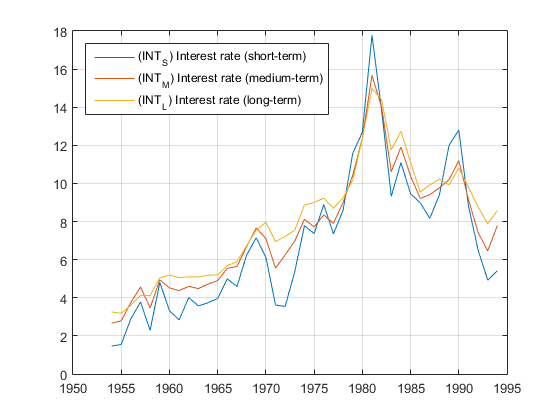
\includegraphics[width=1\textwidth]{TestMultipleSeriesForCointegrationUsingJcitestExample_01}
        \caption{Cointegration of the interest rates (short, medium and long-term) in Canada from 1955 to 1995}
        \label{TestMultipleSeriesForCointegrationUsingJcitestExample_01}
    \end{subfigure}
    \begin{subfigure}[t]{0.49\textwidth}
        \centering
        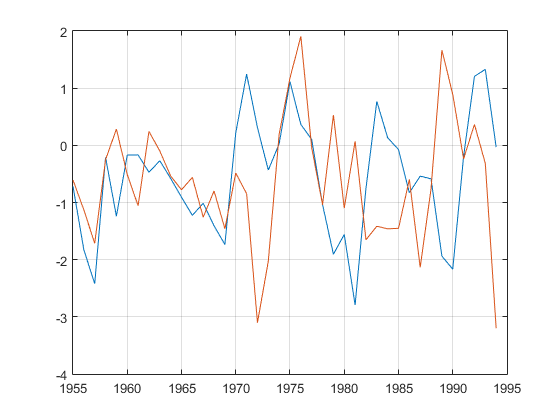
\includegraphics[width=1\textwidth]{TestMultipleSeriesForCointegrationUsingJcitestExample_02}
        \caption{Estimated Cointegrating relations $\beta' y_{t-1} + c_0$}
        \label{TestMultipleSeriesForCointegrationUsingJcitestExample_02}
    \end{subfigure}
    \caption{Cointegration Property of Canadian interest rates}
\end{figure}

It seems that the existence of more than one cointegrating vectors (i.e. the long-run relationship) is not necessarily a good sign, since there is uncertainty as to which relationship the variables will obey in the long and short run. The dynamics may be unstable.

\section{Testing for Unit Roots in Stochastic Processes}

% PP TEST doc very interesting
Before testing for a unit root, i.e. if the series is $I(1)$, the time series must be transformed to its linear form. Usually, assets prices have an exponential growth and logarithm should be applied accordingly to satisfy this prerequisite. Once the data is transformed, we must choose the most pertinent model to use in the Augmented Dickey Fuller and Philipps-Perron tests. There are three basic models for economic data $(Y_t)_{t>0}$ with linear growth characteristics
%http://uk.mathworks.com/help/econ/adftest.html#inputs
\begin{itemize}
\item Trend Stationary model variant (TS) \\
H0: $y_t = c + y_{t-1} + \phi_1 \Delta y_{t-1} + \cdots + \phi_p \Delta y_{t-p} + \epsilon_t $ \\
H1: $y_t = c \delta t + \gamma y_{t-1} + \phi_1 \Delta y_{t-1} + \cdots + \phi_p \Delta y_{t-p} + \epsilon_t $ \\
with drift coefficient $c$, deterministic trend coefficient $\delta$ and $AR(1)$ coefficient $\gamma <1$.
\item Auto Regressive with Drift variant (ARD) \\
H0: $y_t = y_{t-1} + \phi_1 \Delta y_{t-1} + \cdots + \phi_p \Delta y_{t-p} + \epsilon_t $ \\
H1: $y_t = c + \gamma y_{t-1} + \phi_1 \Delta y_{t-1} + \cdots + \phi_p \Delta y_{t-p} + \epsilon_t $ \\
with drift coefficient $c$, and $AR(1)$ coefficient $\gamma <1$.
\item Auto Regressive variant (AR) \\
H0: $y_t = y_{t-1} + \phi_1 \Delta y_{t-1} + \cdots + \phi_p \Delta y_{t-p} + \epsilon_t $ \\
H1: $y_t = \gamma y_{t-1} + \phi_1 \Delta y_{t-1} + \cdots + \phi_p \Delta y_{t-p} + \epsilon_t $ \\
with $AR(1)$ coefficient $\gamma <1$.
\end{itemize}

%http://uk.mathworks.com/help/econ/unit-root-nonstationarity.html Choose Models to Test
$\epsilon_t$ is a mean zero innovation process. In general, if the series is growing, the TS model provides a reasonable trend-stationary alternative to a unit-root process with drift. If the series shows no trend but has a non zero mean, the ARD model provides reasonable stationary alternatives to a unit-root process without drift. Finally, if the series has no trend and a zero mean, the AR model is the most suitable. As the spread is a non zero mean without any drift, the ARD model is the best alternative model for testing. \\

%https://tel.archives-ouvertes.fr/hal-01020405/document
The next step is to determine the number of lags to include in the model. Different criteria used for lag length often lead to different decisions regarding the optimal lag order that should be used in the model. \cite{daoimpact} suggested a general procedure for the ADF test
\begin{itemize}
\item Determine the optimal max lag value denoted $L_{max}$. It is clear that $L_{min} = 0$ is the minimum value of lag length that could be used. \cite{schwert2002} suggested to use $L_{max} = 12 \left(T / 100 \right)^{1/4}$ where $T$ is the length of the time series. It guarantees that $L_{max}$ grows with $T$.
\item When $L_{min}$ and $L_{max}$ are established, ADF t-statistics are calculated for all lag length values between the range $(L_{min}, L_{max})$. The most negative value from all ADF t-statistics indicates the value of lag length that produces the most stationary residuals.
\end{itemize}
% The general method to find the optimal lag for the Phillips-Perron test is to begin with few lags, and then evaluate the sensitivity of the results by adding more lags. Another rule of thumb is to look at sample autocorrelations of $\Delta y_t = y_t - y_{t-1}$. Slow rates of decay require more lags. It is less suitable for economic data because it is widely known that the returns $\Delta y_t$ show no autocorrelation. Finally, when the optimal lags are known, multiple tests are run to avoid any possible inconsistency.

\chapter{State-Space Models and Stochastic Volatility}
\section{State-Space Models}
\label{section:ssm}
The term \textit{state space} originated in 1960s in the area of control engineering - \cite{kalman1960}. State space model refers to a class of probabilistic graphical model that describes the probabilistic dependence between the latent state variables $\matr{x}_{1:T}$ and the observed measurements $\matr{y}_{1:T}$. The system evolves according to
\begin{align*}
\matr{X}_t &= f_\theta(\matr{X}_{t-1},\matr{W}_{t-1}) \numberthis \label{system_equation} \\
\matr{Y}_t &= h_\theta(\matr{X}_t, \matr{V}_t) \numberthis \label{measurement_equation}
\end{align*}
where, $\matr{X}_t \in \mathbb{R}^n$ is the state vector and $\matr{Y}_t \in \mathbb{R}^n$ is the measurement vector. $f_\theta$ is a Markov process of order one and $h_\theta$ is a non-linear. Both are time invariant and deterministic. $\matr{W}_t$ is the i.i.d. system noise sequences and $\matr{V}_t$ the i.i.d. measurement noise sequences. \\

Equation (\ref{system_equation}) is known as the system equation and Equation (\ref{measurement_equation}) is known as the measurement equation. We assume that the process generating the system states $\matr{X}_t$ and thus the observed states $\matr{Y}_t$ starts from an initial value $\matr{x}_1$. In some models we consider, we make additional assumptions about the noise processes. The joint process $(\matr{W}_t, \matr{V}_t)_{t>0}$ is a zero mean, serially uncorrelated noise process with possibly time varying covariance matrices
\begin{equation}
\begin{pmatrix}
\Sigma_{\matr{W}_t} & \Sigma_{\matr{W}_t, \matr{V}_t}\\
\Sigma_{\matr{V}_t, \matr{W}_t} & \Sigma_{\matr{V}_t} \label{corr_ssm}
\end{pmatrix}
\end{equation}
The Directed Acyclic Graph for this state-space is given in Figure \ref{state_space_models}.
\begin{figure}[H]
\centering
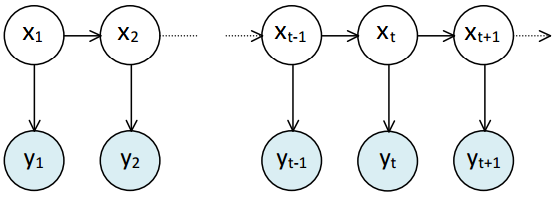
\includegraphics[width = 0.75\textwidth]{state_space_models}
\caption{DAG for the state-space model with first order Markov latent dynamics}
\label{state_space_models}
\end{figure}

$f_\theta$ and $h_\theta$ are parametrised by $\theta = (\theta_1,...,\theta_n)^T$ and each $\theta_i$ is assumed to be independent from $(\theta_j)_{j \neq i}$. A prior distribution $p(\theta) = \prod_i p(\theta_i)$ is associated to the parameter $\theta$. With the stochastic assumptions mentioned above, the probability density of $\matr{X}_{1:T}$ is written as
\begin{equation}
p(\matr{x}_{1:T} | \theta) = p(\matr{x}_1|\theta) \prod_{t=2}^T p(\matr{x}_t|\matr{x}_{t-1}, \theta) 
\end{equation}

The realization $\matr{x}_{1:T}$ is not observed directly, but through $\matr{y}_{1:T}$. The state-space model assumes that each observation $\matr{y}_t$ is statistically independent of every other quantity except $\matr{x}_t$ and $\theta$, through Equation (\ref{measurement_equation}). As a consequence, the conditional likelihood of the observations, given the state process can be derived as
\begin{equation}
p(\matr{y}_{1:T} | \matr{x}_{1:T}, \theta) = \prod_{t=2}^T p(\matr{y}_t | \matr{x}_t, \theta) = \int p(\matr{y}_t|\matr{x}_t, \theta) d\matr{y}_t
\end{equation}
where $d \matr{y}_T$ is the Lebesgue measure.
Here $\theta$ is treated as unknown and the general idea is to estimate it using Maximum Likelihood Estimation (MLE) on the marginal likelihood $p(\matr{y}_{1:T}|\theta)$, with the latent variables $\matr{x}_{1:T}$ integrated out
\begin{equation}
p(\matr{y}_{1:T} | \theta) = p(\matr{y}_1 |\theta) \prod_{t=2}^T p(\matr{y}_t | \matr{y}_{1:t-1}, \theta) = \int p(\matr{y}_T|\matr{x}_T, \theta) p(\matr{x}_T|\matr{y}_{1:T-1}, \theta) d \matr{x}_T\label{intractable_ssm_2}
\end{equation}
It is also interesting to consider the approximation of the latent variables $p(\matr{x}_{1:T}, \theta | \matr{y}_{1:T})$. By Bayes theorem,
\begin{align*}
p(\matr{x}_{1:T}, \theta | \matr{y}_{1:T}) &= \frac{ p(\theta)p(\matr{x}_{1:T}|\theta)p(\matr{y}_{1:T}|\matr{x}_{1:T}, \theta) }{p(\matr{y}_{1:T})}\numberthis \label{intractable_ssm}
\end{align*}
where
\begin{equation}
p(\matr{y}_{1:T}) = \int p(\matr{y}_{1:T}|\theta')p(\theta') d\theta' = \int \int p(\matr{y}_T|\matr{x}_T, \theta') p(\matr{x}_T|\matr{y}_{1:T-1}, \theta') p(\theta') d \matr{x}_T d\theta'
\end{equation}

In most cases, $p(\matr{x}_{1:T}, \theta | \matr{y}_{1:T})$ is hard to compute because $p(\matr{y}_{1:T} | \theta)$ is analytically intractable. When $\theta$ is known, the problem of inference in the path space is effectively addressed using Sequential Monte Carlo methods. However, despite the success of standard SMC methods, the general case of the joint inference on $\theta$ and on $\matr{x}_{1:T}$ for a generic, non-linear non-Gaussian, state-space model is a very challenging problem, which, although extremely important for a wide variety of applications, is still somewhat unresolved. To attempt to overcome these difficulties, \cite{andrieu2010} developed \textit{Particle Markov Chain Monte Carlo} algorithms. These are MCMC algorithms which use a particle filter to estimate the intractable true value of (\ref{intractable_ssm_2}). It is presented in more depth in Section\ref{section:pmcmc}.

\section{Stochastic Volatility Models}
\label{sec:sv}
The most important feature of the conditional return distribution $y_t | \mathcal{F}_{t-1}$ is its variance dynamics. The first research on modelling this volatility was \cite{engle1982} with the famous ARCH model. The main objective was to fit volatility clustering and the fat tails of the return distributions. In this section, we introduce the standard stochastic volatility model (denoted $\mathcal{M}_1$) and its different extensions. The first extension $\mathcal{M}_2$ consists in replacing the Gaussian errors with Student-t errors. In the second extension called $\mathcal{M}_3$, we incorporate a leverage effect by modelling a correlation parameter between measurement and state errors. In $\mathcal{M}_4$, we implement a model to check if that the measurement errors are serially independent. $\mathcal{M}_5$ makes the assumption that the conditional mean is somehow proportional to the conditional volatility. Finally, the last extensions $\mathcal{M}_6$ and $\mathcal{M}_7$ incorporate two latent processes to model the volatility of the returns. $\mathcal{M}_7$ introduces a leverage on one of its latent process. It is also worth mentioning that the processes considered in this section are assumed to be univariate.

\subsection{Model $\mathcal{M}_1$ - Standard Stochastic Volatility Model (SV)}
The standard discrete-time stochastic volatility model for the asset prices returns $(Y_t)_{t>0}$ is defined as
\begin{align*}
  X_t &=  \phi X_{t-1} + \sigma \epsilon_{X,t-1} \numberthis \label{std_SV_process_X} \\
  Y_t &=  \beta \exp \left( \frac{X_t}{2} \right) \epsilon_{Y,t} \numberthis
\end{align*}
where $(\epsilon_{X,t})_{t>0},(\epsilon_{Y,t})_{t>0}$ are two independent and standard normally distributed processes. Let $\theta = (\rho, \sigma^2, \beta)$ be the parameters vector. This model is non-linear because of the non-additive noise of the transition kernel. $(X_t)_{t>0}$ governs the volatility process of the observed returns $(Y_t)_{t>0}$, $\sigma$ is the volatility of the volatility, and $\phi$ the persistence parameter. The condition $|\phi| < 1$  is imposed to have a stationary process, with initial condition $X_0 \sim \mathcal{N} \left(0, \frac{\sigma^2}{1-\phi^2} \right)$, where $\frac{\sigma^2}{1-\phi^2}$ is the unconditional variance of $(X_t)_{t>0}$. The next part explains the link between the stochastic volatility model and the Geometric Brownian Motion (GBM).

%https://en.wikibooks.org/wiki/LaTeX/Theorems
\begin{definition}
\textit{
A stochastic process $S_t$ is said to follow a Geometric Brownian Motion if it satisfies the following stochastic differential equation
$dS_t = \mu S_t dt + \sigma S_t dW_t$
where $W_t$ is a Wiener process, $\mu$ the drift and $\sigma$ the volatility. Both $\mu$ and $\sigma$ are assumed to be constant.}
\end{definition}

The process can be discretized by
\begin{align*}
S_{t+1}-S_t &= \mu S_t + \sigma S_t \epsilon_{t+1} \text{, } \epsilon_{t} \sim \mathcal{N}(0,1) \\
S_{t+1} 	&= S_t + \mu S_t + \sigma S_t \epsilon_{t+1} \\
S_t 	&= S_{t-1} + \mu S_{t-1} + \sigma S_{t-1} \epsilon_t \numberthis
\end{align*}

In the Stochastic Volatility model (SV), $(Y_t)_{t>0}$ represents the returns of the modelled asset. A general definition for computing the returns is $y_t = S_t / S_{t-1} - 1$, where $(S_t)_{t>0}$ is the asset observed prices. When $x_t$ is measured at time $t^-$ with regard to the filtration $\mathcal{F}_{t^-}$, $(Y_t|X_t = x_t)_t$ is normally distributed as
\begin{align*}
Y_t | X_t = x_t, \theta 					&\sim \mathcal{N}(0, \beta^2 \exp(x_t)) \\
%\frac{S_t}{S_{t-1}}-1 | X_t = x_t, \theta 	&\sim \mathcal{N}(0, \beta^2 \exp(x_t)) \\
%\frac{S_t}{S_{t-1}} | X_t = x_t, \theta 	&\sim \mathcal{N}(1, \beta^2 \exp(x_t)) \\
S_t | X_t = x_t, \theta 					&\sim \mathcal{N}(S_{t-1}, \underbrace{S_{t-1}^2 \beta^2 \exp(x_t)}_{\sigma^2(t)}) \numberthis \label{cond_dist_sv_model}
\end{align*}


 The variance $\sigma^2(t)$ always exists as a product of square and exponential terms. Finally, $S_t = S_{t-1} + \sigma(t) S_{t-1} \epsilon_t \text{, } \epsilon_t \sim \mathcal{N}(0,1)$ corresponds to the discretized Geometric Brownian Motion equation with $\mu = 0$ if and only if $\sigma(t) = \sigma \text{, } \forall t > 0$. The interest of using a Stochastic Volatility model essentially relies on the capability of modelling this volatility.

\subsection{Model $\mathcal{M}_2$ - Stochastic Volatility Student-t (SVt)}
The first extension is a stochastic volatility model with heavier tails where $\epsilon_{Y,t} \sim t(\nu)$. $\theta$ is enriched with the new parameter $\nu$, supposed to be unknown.

\begin{lemma}
\textit{
Assume that $X$ is a random variable of probability density function $f_X(x)$. The probability density function $f_Y(y)$ of $Y=g(X)$ where $g$ is monotonic, is given by
}
\begin{equation}
f_Y(y) = \left|\frac{d}{dy}(g^{-1}(y))\right| \cdot f_X(g^{-1}(y))
\end{equation}
\end{lemma}


Applying this lemma on $y_t = \sigma(t) \epsilon_{Y,t}$ where $\sigma(t) = \beta \exp \left(\frac{x_t}{2} \right)$ and $g^{-1}_t(x) = \frac{x}{\sigma(t)}$ gives,

\begin{equation}
p(y_t | X_t = x_t, \theta) = \frac{\Gamma(\frac{\nu+1}{2})}{\Gamma(\frac{\nu}{2}) \sqrt{\nu\pi}} \frac{1}{\sigma_t}\left( 1 + \frac{y_t^2}{\sigma_t^2 \nu}\right)^{-\left(\frac{v+1}{2} \right)}
\end{equation}
where $\Gamma(\cdot)$ is the gamma function. This result can also be retrieved by considering the $t$ location-scale distribution with parameters $(\mu = 0, \sigma, \nu)$, whose probability density function is given by
\begin{equation}
\frac{\Gamma \left(\frac{\nu+1}{2} \right)}{\sigma \sqrt{\pi \nu} \Gamma \left(\frac{\nu}{2} \right)} \left[ \frac{\nu + \left( \frac{x-\mu}{\sigma}\right)^2}{\nu}\right]^{-\left(\frac{\nu+1}{2} \right)}
\end{equation}


The reasoning to find a closed form of $(S_t | x_t)$ is similar to the standard stochastic volatility model. Still under the assumption that $\epsilon_{Y,t} \sim t(\nu)$, if $X$ has a $t$ location-scale distribution, with parameters $\mu, \sigma, \nu$, then $\frac{x-\mu}{\sigma}$ has a Student's $t$ distribution with $\nu$ degrees of freedom. Reverting the equation yields $x = \mu + \sigma \epsilon_{Y,t}$. Consequently,
\begin{align*}
S_t  &= \underbrace{S_{t-1}}_{\mu(t)} + \underbrace{\beta S_{t-1} \exp \left( \frac{x_t}{2} \right)}_{\sigma(t)} \epsilon_{Y,t} \numberthis
\end{align*}
As a conclusion, $(S_t | x_t, \theta)_{t>0}$ follows a $t$ location-scale distribution of parameters $(\mu(t), \sigma(t), \nu)$.

\subsection{Model $\mathcal{M}_3$ - Stochastic Volatility Leverage (SVL)}
In the second extension, a leverage effect is added. \cite{black1976} discovered that most measures of volatility of an asset are negatively correlated with the returns of that asset. It is considered nowadays as a stylized fact in econometrics series. Let $\rho$ denote the correlation between the innovation processes $(\epsilon_{X,t})_{t>0}$ and $(\epsilon_{Y,t})_{t>0}$. $\theta$ is enriched with the new parameter $\rho$.

\begin{lemma}
\textit{
[Cholesky Decomposition] Let $X$, $Y$ be two standard normally distributed random variables. The correlation between X and Y is $\rho$ if and only if $Y = \rho X + \sqrt{1-p^2} Z$ where $Z \sim \mathcal{N}(0,1)$ and is independent of both $X$ and $Y$.
}
\end{lemma}
Applying the Cholesky decomposition on the innovations gives $\epsilon_{X,t} = \rho \epsilon_{Y,t} + \sqrt{1-\rho^2} Z$. This identity is helpful when it comes to generate artificial datasets from this model. It is worth noting that $\epsilon_{Y,t}$ is first measured and $\epsilon_{X,t}$ is updated accordingly. It means that $\epsilon_{Y,t}$ is independent from all the past values $(\epsilon_{X,s})_{s < t}$. Consequently, the conditional distributions of $Y_t$ and $S_t$ remain unchanged from Equation (\ref{cond_dist_sv_model}).

% \begin{align*}
% Y_t 								&= \beta \exp \left(\frac{x_t}{2}\right) \cdot \left( \rho \epsilon_{X,t} + \sqrt{1-\rho^2} Z \right) \\
% Y_t 								&= \beta \exp \left(\frac{x_t}{2}\right)  \rho \epsilon_{X,t} + \beta \exp \left(\frac{x_t}{2}\right) \sqrt{1-\rho^2} Z \\
% \frac{S_t}{S_{t-1}}-1 | X_t = x_t 					&\sim \mathcal{N} \left(\beta \rho \exp \left(\frac{x_t}{2}\right) \epsilon_{X,t}, \beta^2 \exp \left(x_t\right) \cdot (1-\rho^2) \right) \\
% \frac{S_t}{S_{t-1}} | X_t = x_t 	&\sim \mathcal{N}\left(1 + \rho \beta \exp \left(\frac{x_t}{2} \right) \epsilon_{X,t}, \beta^2 \exp(x_t) \cdot (1-\rho^2)\right) \\
% S_t | X_t = x_t 					&\sim \mathcal{N}\left( S_{t-1} + S_{t-1} \rho \beta \exp \left(\frac{x_t}{2} \right) \epsilon_{X,t}, S_{t-1}^2 \beta^2 \exp(x_t) \cdot (1-\rho^2)\right) \numberthis
% \end{align*}
% The differences between the normal leverage model and the standard model where $\rho = 0$, are the correcting drift term $S_{t-1} \rho \beta \exp \left(\frac{x_t}{2} \right) \epsilon_{X,t}$ and the factor $(1-\rho^2) \leq 1$ reducing the volatility.

%http://people.anu.edu.au/joshua.chan/Chan-Hsiao-2013.pdf
\subsection{Model $\mathcal{M}_4$ - SV-MA(1) - Moving Average (SVMA)}
The standard stochastic volatility model assumes that the errors in the measurement equation are serially independent. This is often an appropriate assumption for modelling financial data. To test this assumption, the plain model can be extended by allowing the errors in the measurement equation to follow a moving average (MA) process of order $m$. Here, we choose a more simple specification and set $m = 1$. Hence, our model becomes
\begin{align*}
Y_t									      &= \beta \exp \left( \frac{X_t}{2} \right) \epsilon_{Y,t} + \psi \beta \exp \left( \frac{X_{t-1}}{2} \right) \epsilon_{Y,t-1} \numberthis \\
Y_t	| \mathcal{F}_{t^-}		&\sim \mathcal{N} \left(0, \beta^2 \exp \left( x_t \right) + \psi^2 \beta^2 \exp \left( x_{t-1} \right) \right) \\
S_t | \mathcal{F}_{t^-}	  &\sim \mathcal{N} \left(S_{t-1}, S_{t-1}^2 \beta^2 \exp \left( x_t \right) +  S_{t-1}^2 \psi^2 \beta^2 \exp \left( x_{t-1} \right) \right) \numberthis
\end{align*}
where the process $X$ is defined in Equation (\ref{std_SV_process_X}). As before, we ensure that the root of the characteristic polynomial associated with the MA coefficient $\psi$, is outside the unit circle: $|\psi| < 1$. When $\psi = 0$, the SV-MA(1) model is reduced to the standard stochastic volatility model. The conditional
variance of $Y_t$ is given by $\var \left(Y_t | \mathcal{F}_{t^-} \right) = \beta^2 e^{x_t} + \beta^2 \psi^2 e^{x_{t-1}}$. The conditional variance is time-varying through two channels: a moving average composed of the two most recent variances $\beta^2 e^{x_t}$ and $\beta^2 e^{x_{t-1}}$ and secondly, according to the stationary $AR(1)$ process $X$.

\subsection{Model $\mathcal{M}_5$ - Stochastic Mean (SVM)}
\cite{koopman2002} suggested an extension where the stochastic volatility also enters into the conditional mean equation. This model is known as the Stochastic Volatility in Mean (SVM). It is defined as
\begin{align*}
Y_t 			 &= \beta \exp\left(\frac{X_t}{2}\right) + \exp\left(\frac{X_t}{2}\right) \epsilon_{Y,t} \numberthis\\
%Y_t | X_t = x_t  &\sim \mathcal{N} \left(\beta \exp\left(\frac{x_t}{2}\right) , \exp\left(x_t\right) \right) \numberthis\\
S_t | \mathcal{F}_{t^-}  &\sim \mathcal{N} \left(S_{t-1} + S_{t-1} \beta \exp\left(\frac{x_t}{2}\right), S_{t-1}^2 \exp\left(x_t\right) \right) \numberthis
\end{align*}
where $X$ corresponds to the process of a standard stochastic volatility model defined in Equation (\ref{std_SV_process_X}). This model is pertinent if we believe that the conditional mean is somehow proportional to the conditional volatility. This can be the case in financial data, where high volatility appears in clusters where the absolute conditional mean is high.

\subsection{Model $\mathcal{M}_6$ - Two Factors Stochastic Volatility (TFSV)}
With a principal component analysis, \cite{harvey1994} showed that a short-run and a long-run factors might be enough to explain the returns volatility. The study was performed on daily observations on several exchange rates. This model is known as the two factor stochastic volatility and relies on two different latent processes $X$ and $Z$. It is defined as
\begin{align*}
  X_t 						&=  \phi_X X_{t-1} + \sigma_X \epsilon_{X,t-1} &|\phi_X| < 1, \epsilon_{X,t-1} \sim \mathcal{N}(0,1), X_1 \sim \mathcal{N} \left(0, \frac{\sigma_X^2}{1 - \phi_X^2} \right) \numberthis \label{tfsv_process_X} \\
  Z_t 						&=  \phi_Z Z_{t-1} + \sigma_Z \epsilon_{Z,t-1} &|\phi_Z| < 1, \epsilon_{Z,t-1} \sim \mathcal{N}(0,1), Z_1 \sim \mathcal{N} \left(0, \frac{\sigma_Z^2}{1 - \phi_Z^2} \right) \numberthis\\
  Y_t 						&=  \beta \exp \left( \frac{X_t+Z_t}{2} \right) \epsilon_{Y,t} &\epsilon_{Y,t} \sim \mathcal{N}(0,1) \numberthis
\end{align*}
Under these assumptions, the conditional distribution of the spread is $S_t | \theta, X_t = x_t, Z_t = z_t \sim \mathcal{N}\left(S_{t-1}, S_{t-1}^2 \beta^2 \exp \left(x_t + z_t\right) \right)$. The parameters vector $\theta$ is now $(\beta, \phi_X, \phi_Z, \sigma_X, \sigma_Z)$ where $\beta$ is a scaling term. It is of common knowledge that the returns are leptokurtic, i.e. with a positive kurtosis. \cite{veiga2006} showed that the second term introduced in the model helps generate extra kurtosis and accounts for short-run dynamics. Also, \cite{chernov2000} found that SV models with one volatility factor are not able to characterize all moments of asset return distributions. In particular, the fat tails of the return distribution are captured rather poorly. \\
Estimating these parameters using \textit{Particle Markov Chain Monte Carlo} is fairly straightforward. The particle filter must be updated such that two sets of particles (one for $X$ and one for $Z$) must be drawn instead of one. Because of the symmetry between $X_t$ and $Z_t$ in $Y_t$, some conditions on the parameters have to be set to ensure the convergence, such that $\phi_X > \phi_Z$.

\subsection{Model $\mathcal{M}_7$ - Two Factors Stochastic Volatility with Leverage (TFSVL)}

In the final extension, we consider the two factors stochastic volatility with a correlation $\rho = cor(\epsilon_{X,t}, \epsilon_{Y,t})$. The idea is the same as the one developed for the model $\mathcal{M}_3$. We assume a non-zero correlation between the innovations of the returns and the long-run factor $X$ from Equation (\ref{tfsv_process_X}). From the models presented before, this model is by far the most complex because 6 parameters are to be estimated: $\theta = (\beta, \rho, \phi_X, \phi_Z, \sigma_X, \sigma_Z)$. \cite{ruiz2008} studied a slightly different version with $X$ defined as a fractional integrated Gaussian noise process (ARFIMA). They proved that the first order autocorrelation $cor(|y_t|,|y_{t+1}|)$ is smaller than the second order autocorrelation $cor(y_t^2,y_{t+1}^2)$ when $\rho < 0$. As explained by \cite{cont2005}, it is usually the case in practical applications. If $\rho = 0$, there is no more asymmetry in the model. From the same considerations as in model $\mathcal{M}_3$, the conditional distributions of $Y_t$ and $S_t$ remains unchanged compared to model $\mathcal{M}_6$.

\chapter{Sequantial Monte Carlo and Particle MCMC}
\label{section:pmcmc}
\section{Introduction}
Many problems involve making inference on unknown parameters of complex models which have a sequential, if not explicitly temporal, basis. \\

\textit{Sequential Monte Carlo} (SMC) are a collection of simulation-based techniques for computing a recursive series of posterior distributions over such complex models. SMC methods are very flexible, relatively easy to implement, parallelizable and application a very wide variety of settings. Since computing power has become so readily available, and due to certain recent advanced in applied statistics, these methods have recently become a mainstay of advanced research methods in this field. Section \ref{section:smc} explains the SMC methods, also known as Particle Filtering. \\

\textit{Particle Markov Chain Monte Carlo} (Particle MCMC) are powerful techniques for estimating parameters of a complex model where classical methods such as maximum likelihood estimation are limited. This is the case for state-space models which incorporate latent variables. Particle MCMC embeds a particle filter of size $N$ within an MCMC scheme. The standard version uses a particle filter to provide an estimate of the intractable marginal likelihood $p(\matr{y}_{1:T}|\theta)$, and MCMC moves to propose new values for the parameter $\theta$. This concept is presented in more details in Section\ref{section:mcmc_pmmh}.

\section{Sequential Monte Carlo}
\label{section:smc}
Sequential Monte Carlo (SMC) paradigm is based on rejection sampling and importance sampling techniques. This section follows the same notations as in Chapter \ref{section:ssm} where the state-space models are defined. The Sequential Importance Sampling (SIS) algorithm is a Monte Carlo method that forms the basis for most sequential Monte Carlo filters. The SIS algorithms alternates the mutation and correction steps of the typical SMC algorithm, but does not perform a selection stage (known as resampling). As such, the importance weights are initialized to one at each iteration and are updated recursively. It turns out that this algorithm has a big drawback, known as the degeneracy problem. In a nutshell, it happens when $T$ is large enough. As the weights are sequentially multiplied and strictly less than 1, they converge to 0 fast. The resulting particles paths are said to be degenerated. In 1987, the Sequential Importance sampling Resampling (SIR) algorithm is introduced. The new content behind the SIR algorithm is to insert a resampling step between two importance sampling steps in the Sequential Importance Sampling (SIS) algorithm. The resampling step works to rectify the degeneracy problem by eliminating samples with trivial importance weights and propagating samples with larger weights.

\subsection{Rejection Sampling}
Rejecting sampling is a technique which samples from a target distribution $p(\matr{X})$, known up to a proportional constant, by sampling from another easy to sample proposal distribution $\pi(\matr{X})$. The assumes that there exists a known finite constant $C$ such that $p(\matr{X}) \leq C \pi(\matr{X})$ for every $\matr{x}$. The idea is to draw $\matr{X} \sim \pi$ and accept it as a sample from $p$ with probability $p(\matr{X}) / ( C \pi(\matr{X}))$.

\subsection{Importance Sampling}
Importance sampling (IS) aims to sample a probability distribution in a region of "importance". The idea of importance sampling is to choose a proposal distribution $\pi(\matr{X})$ in place of the true probability distribution $p(\matr{X})$, which is difficult to sample. The support of $\pi(\matr{X})$ is assumed to cover that of $p(\matr{X})$. Under these assumptions, the classic Monte Carlo integration problem
\begin{equation}
p(f) = E[f(\matr{X})] = \int f(\matr{X})p(d\matr{X})
\end{equation}
for any suitable function $f$ can be rewritten as
\begin{equation}
\int f(\matr{X})p(\matr{X})d\matr{X} = \int f(\matr{X}) \frac{p(\matr{X})}{\pi(\matr{X})} \pi(\matr{X}) d\matr{X} \label{is_equation}
\end{equation}
IS is used to draw a number of independent samples from $\pi(\matr{X})$ to obtain an estimate of Equation (\ref{is_equation}). Each sample, $f(\matr{X}_i)$ is assigned an importance weight, $W(\matr{X}_i) \propto p(\matr{X}_i)/\pi(\matr{X}_i)$. In practice, it is important the variance of the importance weights are finite. The proposal distribution $\pi(\matr{X})$ must be as close to possible to $p(\matr{X})$ such that the variance of the weights is minimized. 

\subsection{Sequential Importance Sampling Resampling}
The resampling step is explained in Algorithm \ref{algo-resampling-step}, from iteration $t \rightarrow t+1$.
\begin{algorithm}[H]
\caption{Sequential Importance Sampling Resampling (SISR)}\label{sisr_filter}
\begin{algorithmic}[1]
\For{i from 1 to N}
  \State Sample $j \in [1,N]$ with probabilities proportional to $\{w_{t}^{(1)},..., w_{t}^{(N)}\}$ (mult)
  \State Replace the current particle $i$ with this new one. $x_t^{(i)} \gets x_t^{(j)}$
  \State Re initialize the weight $w_t^{(i)} = 1/N$
\EndFor{end}
\label{algo-resampling-step}
\end{algorithmic}
\end{algorithm}

The general algorithm SISR is presented in Algorithm \ref{algo_sisr_filter}.
\begin{algorithm}[H]
\caption{Sequential Importance Sampling Resampling (SISR)}\label{algo_sisr_filter}
\begin{algorithmic}[1]
\Procedure{Input}{$y_{1:T}$, $\theta$, N}
\For{i from 1 to N}
	\State Sample $x_1^{(i)}$ independently from $p(x_1)$
	\State Calculate weights $w_1^{(i)} = p(y_1 | x_1^{(i)})$
\EndFor{end}
\State $x^*_1 = \sum_{i=1}^N x_1^{(i)}.w_1^{(i)}$
\State Set $\hat{p}(y_1) = \frac{1}{N} \sum_{i=1}^N w_1^{(i)}$

\For{t from 1 to T}
	\For{i from 1 to N}
	  \State Draw sample from the proposal distribution $x_t^{(i)} \sim \pi \left(x_t|x_{0:t-1}^{(i)}, y_{1:t} \right)$
		\State Calculate weight $\displaystyle{\hat{w}_t^{(i)} = w_{t-1}^{(i)} \frac{p(y_t|x_t^{(i)}) p(x_t^{(i)}|x_{t-1}^{(i)})}{\pi \left(x_t^{(i)}|x_{0:t-1}^{(i)}, y_{1:t} \right)}}$
		\State Compute the normalized importance weight $\displaystyle{w_t^{(i)} = \frac{\hat{w}_t^{(i)}}{\sum_{j=1}^N \hat{w}_t^{(j)}}}$
	\EndFor{end}
	\State Compute an estimation of ESS as $N_{eff} = 1 / \left(  \sum_{i=1}^N \left(w_t^{(i)} \right)^2 \right)$
	\If{$N_{eff} < N_{thr}$} 
		  \State //perform resampling step
		\EndIf{end}
	\State $x^*_t = \sum_{i=1}^N x_t^{(i)}.w_t^{(i)}$
	\State Set $\hat{p}(y_{1:t}) = \hat{p}(y_{1:t-1}) \left(\frac{1}{N} \sum_{i=1}^N w_t^{(i)} \right)$
\EndFor{end}
\\
\Return ($x^*_{1:T}$, $\hat{p}(y_{1:T})$)
\EndProcedure
\end{algorithmic}
\end{algorithm}

\subsection{Bootstrap Particle Filter}

% \begin{algorithm}
% \caption{Bootstrap Particle Filtering Algorithm (SIR)}\label{bootstrap_filter_algo}
% \begin{algorithmic}[1]
% \Procedure{Input}{$y_{1:T}$, $\theta$, N}
% \For{i from 1 to N}
% 	\State Sample $x_1^{(i)}$ independently from $p(x_1)$
% 	\State Calculate weights $w_1^{(i)} = p(y_1 | x_1^{(i)})$
% \EndFor{end}
% \State $x^*_1 = \sum_{i=1}^N x_1^{(i)}.w_1^{(i)}$
% \State Set $\hat{p}(y_1) = \frac{1}{N} \sum_{i=1}^N w_1^{(i)}$
% 
% \For{t from 1 to T}
% 	\For{i from 1 to N}
% 		\State Sample $j \in [1,N]$ with probabilities proportional to $\{w_{t-1}^{(1)},..., w_{t-1}^{(N)}\}$
%     \State Replace the current particle $i$ with this new one. $x_t^{(i)} \gets x_t^{(j)}$
% 		\State Sample $x_t^{(i)}$ from $p(x_t|x_{t-1})$
% 		\State Calculate weights $w_t^{(i)} = p(y_t|x_t^{(i)})$
% 	\EndFor{end}
% 	\State $x^*_t = \sum_{i=1}^N x_t^{(i)}.w_t^{(i)}$
% 	\State Set $\hat{p}(y_{1:t}) = \hat{p}(y_{1:t-1}) \left(\frac{1}{N} \sum_{i=1}^N w_t^{(i)} \right)$
% \EndFor{end}
% \\
% \Return ($x^*_{1:T}$, $\hat{p}(y_{1:T})$)
% \EndProcedure
% \end{algorithmic}
% \end{algorithm}

Particle filters with transition prior probability distribution $p_\theta(\matr{X}_t | \matr{X}_{t-1})$ as importance function $\pi(\matr{X})$ are commonly known as bootstrap filter. This choice is motivated by the facility of drawing particles and performing subsequent importance weight calculations. Here, $\pi(\matr{x}_k| \matr{x}_{0:k-1}, \matr{y}_{0:k}) = p(\matr{x}_k|\matr{x}_{k-1})$. Coupled with $N_{thr} = \infty$ (resampling at each step), the weights formula is updated to
\begin{equation}
w_k^{(i)} = \frac{p(\matr{y}_k|\matr{x}_k^{(i)})p(\matr{x}_k^{(i)}|\matr{x}^{(i)}_{k-1})}{\pi(\matr{x}_k^{(i)}|\matr{x}^{(i)}_{0:k-1},\matr{y}_{0:k})}=  p(\matr{y}_k|\matr{x}_k^{(i)})
\end{equation}
It is the most common sequential monte Carlo and provides good results overall. \\
It is clear from our understanding of importance resampling that these weights are appropriate for representing a sample from $p(\matr{x}_{t+1}|\matr{y}_{1:t+1})$, and so the particles and weights can be propagated forward to the next time point. It is also clear that the average weight at each time gives an estimate of the marginal likelihood of the current data point given the data so far. So we define the conditional marginal of $\matr{y}_t$ by

\begin{equation}
 \hat{p}^N_{\theta}(\matr{y}_t | \matr{y}_{1:t-1}) = \frac{1}{N} \sum_{k=1}^N w_t^k
\end{equation}

and the conditional marginal estimator of $y_{1:T}$ over all the state space is
\begin{equation}
 \hat{p}^N_\theta(\matr{y}_{1:T}) = \hat{p}^N_\theta(\matr{y}_1)\prod_{t=2}^T \hat{p}^N_\theta(\matr{y}_t | \matr{y}_{1:t-1}) = \prod_{t=1}^T \left( \frac{1}{N} \sum_{k=1}^N w_t^k \right)
\end{equation}

Again, from the importance resampling scheme, it should be reasonably clear that $\hat{p}^N_{\theta}(\matr{y}_{1:T})$ is a consistent estimator of $p_{\theta}(\matr{y}_{1:T})$. It is much less obvious, but nevertheless true that this estimator is also unbiased, according to \cite{delmoral2004}. This result is the cornerstone of Particle MCMC models. As $T$ is usually large, it is preferred to work with the log likelihoods
\begin{align*}
\log p_{\theta}(\matr{y}_{1:T}) &= \log p_\theta(\matr{y}_1) + \sum_{t=2}^T \log p_\theta(\matr{y}_t | \matr{y}_{1:T-1}) \numberthis \\
\log \hat{p}^N_\theta(\matr{y}_{1:T}) &= \sum_{t=1}^T \log \left(\frac{1}{N} \sum_{k=1}^N w_t^{k} \right) \numberthis
\end{align*}

\section{Resampling step}
As exposed before, Sequential Monte Carlo can be decomposed in two main steps: sequential importance sampling (SIS) and resampling. The main drawback of SIS is that it becomes very unstable as $T$ increases due to the discrepancy between the weights, a phenomenon known as weight degeneracy. To stabilize the algorithm and gain some accuracy, it is necessary to perform resampling sufficiently often. This step is also time-critical as it is on the critical path of the \textit{Particle Markov Chain Monte Carlo} algorithm. We ran benchmarks and it turned out that it can represent more than half of the time spent in the bootstrap filter. Many different methods exist in the literature: multinomial, stratified, systematic and residuals resampling are such examples. In practical applications, \cite{douc2005} found that they provide comparable results. Despite the lack of complete theoretical analysis of its behavior, multinomial resampling is probably the most used algorithm because almost all software products offer a default implementation of this method. In this section, we focus on multinomial and stratified resampling. The mathematical framework is taken from \cite{douc2005}. \\

Denote by $\left( \xi_i, \omega_i \right)_{1 \leq i \leq n, t > 0}$ the set of particle positions and associated weights at time $t$. The filtration $(\mathcal{F}_t)_{t > 0}$ is used to model the information known of the particles and the weights up to time $t$. The weights are assumed to be normalized, i.e. $\forall t > 0, \sum_{i=1}^n \omega_i = 1$. Otherwise, consider $\omega_i \leftarrow \omega_i \text{ /} \sum_{j=1}^n \omega_j$. The resampling step consists in selecting new particle positions and weights $\left( \widetilde{\xi_i}, \widetilde{\omega_i} \right)_{1 \leq i \leq n}$ at time $t+1$ such that the discrepancy between the resampled weights $\widetilde{\omega_i}$ is reduced. There are many possible ways to resample. Two methods are discussed in this section: multinomial and stratified resampling. \\


Multinomial resampling is at the core of the bootstrap method that consists in drawing, conditionally upon $\mathcal{F}_t$, the new positions $\left( \xi_i \right)_{1 \leq i \leq n}$ independently. In practice, this is achieved by repeated uses of the inversion method
\begin{itemize}
\item Draw $n$ independent uniforms $(U^i)_{1 \leq i \leq n}$ on the interval $(0, 1]$.
\item Set $I^i = D_\omega^{inv}(U^i)$ and $\widetilde{\xi_i} = \xi_{I^i}$ where $D_\omega^{inv}$ is the inverse of the cumulative distribution associated with the normalized weights $\left( \omega_i \right)_{1 \leq i \leq n}$, that is $D_\omega^{inv}(u) = i$ for $u \in \left( \sum_{j=1}^{i-1} \omega_j, \sum_{j=1}^i \omega_j \right)$. For better clarity, the function $\xi(i) = \xi_i$ is written as $\xi \circ D_\omega^{inv}(U^i)$.
\end{itemize}
This form of resampling is known as multinomial since the duplication counts are by definition distributed according to the multinomial distribution. \\


Stratified resampling is based on concepts used in survey sampling and consists in pre-partitioning the $(0,1]$ interval into $n$ disjoint sets, $(0,1] = (0, 1/n] \cup \cdots \cup (1-1/n, 1]$. The uniform random variables $U^i$ are then drawn independently in each of these sub-intervals: $U^i \sim \mathcal{U}\left( \frac{i-1}{n}, \frac{i}{n} \right)$. Then, the inversion method is used as in multinomial resampling.

\begin{theorem}
\textit{
Stratified resampling has a lower variance, conditionally upon $\mathcal{F}_t$, than multinomial resampling.
}
\end{theorem}
\begin{proof}
See Appendix \ref{app:proof}.
\end{proof}

From a pure mathematical point of view, the stratified resampling should be preferred. A benchmark study consisting in resampling 1000 weights a large number of times was performed and the results are interesting according to Table \ref{resampling_method_table}. The stratified resampling offers the best balance in terms of speed and intrinsic variance. For those reasons, it is the default resampling method used inside the particle filters.

\begin{table}[H]
\centering
\begin{tabular}{ll}
\hline
\multicolumn{1}{|l|}{Resampling method}     & \multicolumn{1}{l|}{Elapsed Time (average)} \\ \hline
Residual 					   &  18.90 s \\
Stratified   				 &  0.62 s \\
Systematic   				 &  0.63 s \\
Multinomial          &  1.87 s \\
\hline
\end{tabular}
\caption{Time spent to resample $10^5$ times 1000 weights}
\label{resampling_method_table}
\end{table}

\section{Particle Marginal Metropolis-Hastings Algorithm}
\label{section:mcmc_pmmh}

In the classic MCMC scheme, the Metropolis Hastings (MH) algorithm is used to target $p(\theta| \matr{y}) \propto p(\matr{y}|\theta)p(\theta)$ with the ratio
\begin{align*}
\min \left( 1, \frac{p(\theta^\star)}{p(\theta)} \times  \frac{q(\theta|\theta^\star)}{q(\theta^\star|\theta)} \times \frac{p({\matr{y}}|\theta^\star)}{p({\matr{y}}|\theta)} \right) \numberthis \label{classic_mcmc_target}
\end{align*}


where $q(\theta^\star|\theta)$ is the proposal density. As discussed before, the marginal likelihood $p(\matr{y}|\theta) = \int_{\mathbb{R}^T} p(\matr{y}|\matr{x})p(\matr{x}|\theta) d\matr{x}$ is often intractable and the ratio becomes impossible to compute. The simple likelihood-free scheme targets the full joint posterior $p(\theta,\matr{x}|\matr{y})$. Usually the knowledge of the kernel $p_\theta(\matr{x}_t|\matr{x}_{t-1})$ makes $p(\matr{x}|\theta)$ tractable. For instance, a path $\matr{x}_{1:T}$ governed by a linear Gaussian process $\matr{x}_t = \rho \matr{x}_{t-1} + \tau \epsilon_{t-1} \text{, } \epsilon_t \sim \mathcal{N}(0,1)$ can be easily simulated as long as $\rho$, $\tau$ and $\matr{x}_1$ are known quantities. The MH is built in two stages. First, a new candidate $\theta^*$ is proposed from $q(\theta^\star|\theta)$. Then, $\matr{x}^*$ is sampled from $p(\matr{x}^\star|\theta^\star)$. The generated pair $(\theta^\star,\matr{x}^\star)$ is accepted with the ratio

\begin{align*}
\min \left( 1, \frac{p(\theta^\star)}{p(\theta)} \times  \frac{q(\theta|\theta^\star)}{q(\theta^\star|\theta)} \times \frac{p(\matr{y}|{\matr{x}}^\star,\theta^\star)}{p(\matr{y}|{\matr{x}},\theta)} \right) \numberthis
\end{align*}
At each step, $\matr{x}^*$ is consistent with $\theta^*$ because it was generated from $p(\matr{x}^\star|\theta^\star)$. The problem of this approach is that the sampled $\matr{x}^*$ may not be consistent with $\matr{y}$. As $T$ grows, it becomes nearly impossible to iterate over all possible values of $\matr{x}^\star$ to track $p(\matr{y}|\matr{x}^\star,\theta)$. This is why $\matr{x}^*$ should be sampled from $p(\matr{x}^\star|\theta^\star,\matr{y})$. Under this assumption, the ratio now becomes

\begin{align*}
 \min \left(1, \frac{p(\theta^\star)}{p(\theta)}   \frac{p({\matr{x}}^\star|\theta^\star)}{p({\matr{x}}|\theta)}   \frac{q(\theta|\theta^\star)}{q(\theta^\star|\theta)}   \frac{p(\matr{y}|{\matr{x}}^\star,\theta^\star)}{p(\matr{y}|{\matr{x}},\theta)}  \frac{p({\matr{x}}|\matr{y},\theta)}{p({\matr{x}}^\star|\matr{y},\theta^\star)} \right) \numberthis
\end{align*}

Using the basic marginal likelihood identity described in \cite{chib1995}, the ratio is simplified to

\begin{align*}
 \min \left(1, \frac{p(\theta^\star)}{p(\theta)}  \times \frac{p(\matr{y}|\theta^\star)}{p(\matr{y}|\theta)} \times \frac{q(\theta|\theta^\star)}{q(\theta^\star|\theta)} \right) \numberthis
\end{align*}


It is now clear that a pseudo-marginal MCMC scheme for state space models can be derived by substituting $\hat{p}^N_{\theta}(\matr{y}_{1:T})$, computed from a particle filter, in place of $p_{\theta}(\matr{y}_{1:T})$. This turns out to be a simple special case of the particle marginal Metropolis-Hastings (PMMH) algorithm described in \cite{andrieu2010} (Algorithm \ref{algo_pmcmc}). Remarkably $\matr{x}$ is no more present and the ratio is exactly the same as the classical marginal scheme shown before in Equation (\ref{classic_mcmc_target}). Indeed, the ideal marginal scheme corresponds to PMMH when $N \rightarrow \infty$. The likelihood-free scheme is obtained with just one particle in the filter. When $N$ is intermediate, the PMMH algorithm is a trade-off between the ideal and the likelihood-free schemes, but is always likelihood-free when one bootstrap particle filter is used. The PMMH algorithm proposed by \cite{andrieu2010} is an MCMC algorithm for state space models jointly updating $\theta$ and $\matr{x}_{1:T}$. First, a proposed new $\theta^\star$ is generated from a proposal $q(\theta^\star|\theta)$, and then a corresponding $\matr{x}_{1:T}^\star$ is generated by running a bootstrap particle filter using the proposed new model parameters $\theta^\star$, and selecting a single trajectory by sampling once from the final set of particles using the final set of weights. This proposed pair $(\theta^\star,x_{1:T}^\star)$ is accepted using the Metropolis-Hastings ratio

\begin{equation}
\min \left(1, \frac{\hat{p}_{\theta^\star}(\matr{y}_{1:T})}{\hat{p}_{\theta}(\matr{y}_{1:T})} \times \frac{p(\theta^\star)}{p(\theta)} \times \frac{q(\theta|\theta^\star)}{q(\theta^\star|\theta)} \right)
\end{equation} 
where $\hat{p}^N_{\theta^\star}(\matr{y}_{1:T})$ is the particle filter's unbiased estimate of marginal likelihood. Note that the terms $p(\cdot)$ and $q(\cdot|\cdot)$ cancel out when the proposal densities correspond to the respective prior distributions.

\begin{algorithm}[H]
\caption{Particle pseudo marginal Metropolis-Hastings Algorithm}\label{algo_pmcmc}
\begin{algorithmic}[1]
\Procedure{Input}{$\matr{y}_{1:T}$, a proposal distribution $q(\cdot|\cdot)$, the number of particles $N$, the number of MCMC steps $M$}

\State $\hat{p}^N_{\theta^{(1)}}(\matr{y}_{1:T}), \matr{x}^{*(1)}_{1:T} \gets$ Call Bootstrap Particle Filter with $(\matr{y}_{1:T}, \theta^{(1)}, N)$

\For{i from 2 to M}
	\State Sample $\theta'$ from $q(\theta|\theta^{(i-1)})$
	\State $\hat{p}^N_{\theta'}(\matr{y}_{1:T}), \matr{x}^{*'}_{1:T}$ $ \gets$ Call Bootstrap Particle Filter with ($\matr{y}_{1:T}$, $\theta'$, N)
	\State With probability,
	
	$$\min \left\{1, \frac{q(\theta^{(i-1)}|\theta')\hat{p}_N(\matr{y}_{1:T}|\theta')p(\theta')}{q(\theta'|\theta^{(i-1)})\hat{p}_N(\matr{y}_{1:T}|\theta^{(i-1)})p(\theta^{(i-1)})}  \right\} $$
	
	\State Set $\matr{x}^{(i)*}_{1:T} \gets \matr{x}^{'*}_{1:T},\theta^{(i-1)} \gets \theta', \hat{p}^N_{\theta^{(i)}}(\matr{y}_{1:T}) \gets \hat{p}^N_{\theta'}(\matr{y}_{1:T})$
	\State Otherwise $\matr{x}^{(i)*}_{1:T} \gets \matr{x}^{(i-1)*}_{1:T},\theta^{(i-1)} \gets \theta^{(i-1)}, \hat{p}^N_{\theta^{(i)}}(\matr{y}_{1:T}) \gets \hat{p}^N_{\theta^{(i-1)}}(\matr{y}_{1:T})$
	
\EndFor{end}
\\
\EndProcedure
\Return $(\matr{x}^{(i)*}_{1:T}, \theta^{(i)})_{i=1}^M$

\end{algorithmic}
\end{algorithm}

Due to the unbiasedness property of $\hat{p}^N_{\theta^\star}(\matr{y}_{1:T})$, the PMMH algorithm works for any positive $N$. In practical applications, a critical issue resides in how to choose the number of particles $N$. A large $N$ gives a more accurate estimate of the log likelihood at a greater computational cost, while a small $N$ would lead to a very large estimator variance.

\section{Tuning the number of particles}
\label{sec:tuning_n}
%http://arxiv.org/pdf/1309.3339v3.pdf p2
\cite{tran2014} showed that the efficiency of estimating an intractable likelihood using Bayesian inference and importance sampling is weakly sensitive to $N$ around its optimal value. Furthermore, the loss of efficiency decreases at worse linearly when we choose $N$ higher than the optimal value, whereas
the efficiency can deteriorate exponentially when $N$ is below the optimal. \cite{pitt2012} showed that we should choose $N$ so that the variance of the resulting log-likelihood is around 0.85. Of course, in practice this variance will not be constant, as it is a function of the parameters as well as a decreasing function of $N$. \cite{pitt2012} suggests that a reasonable strategy is to estimate the posterior mean $\bar{\theta} = E[\theta|y_{1:T}]$ from an initial short run of the PMCMC scheme with $N$ set to a large value. The value of $N$ could then be adjusted such that the variance of the log-likelihood Var$(\log p_N(y|\bar{\theta}))$ evaluated at $\bar{\theta}$ is around 0.85. The penalty for getting the variance wrong is not too severe within a certain range. Still from \cite{pitt2012}, their results indicated that although a value of $0.92^2 = 0.8464$ is optimal, the penalty is small provided the value is between 0.25 and 2.25. This allows for quite a large margin of error in choosing $N$ and also suggests that the simple schemes advocated should work well. \\
An analysis was carried out to measure the variations of the variance across the parameter space and for different values of $N$. The state-space model $\mathcal{M}_2$ is used to generate an artificial dataset with $(\rho,\sigma,\nu) = (0.91,1,3)$. The bootstrap filter is called repeatedly to estimate its intrinsic variance. Figure (\ref{tuning_n_rho_varying}) shows the behavior of the filter's variance $\var(\log \hat{p}_N(y|\theta))$ when $\rho$ varies over its domain of definition. It gives a hint that the variance is not likely to oscillate in big proportions when the model parameters $\theta$ change. \\

The reasonable strategy of \cite{pitt2012} is not viable in practice as it requires to have a good estimate of $\bar{\theta}$ which is often difficult to achieve with a short run of PMCMC due to the burn-in phase. It is much more relevant to derive a general rule on how to choose $N$ optimal, provided that such a rule exists. A test is conducted on an artificial dataset where the true value $\theta_{tr} = \bar{\theta}$ is known. It is composed of $T=1000$ daily returns, generated from model $\mathcal{M}_2$. For a given value of $N$, the bootstrap filter of $\mathcal{M}_2$ is called several times and the variance of the log likelihoods Var$(\log p_N(y|\bar{\theta}))$ is estimated. The process is repeated for different values of $N$. From Figure (\ref{est_var_pn_theta_n}), the optimal of $N$ seems to be around 1000. The process is repeated for several values of $T$ to detect a general rule. Figure \ref{n_opt_function_t} shows the results for $T \in [0, 2000]$ and $N \in [0, 2500]$. A linear trend can easily be identified. To reinforce this belief, a linear regression $N = a T + b$ is performed. Both the values $b \simeq 0 (3)$ and $a \simeq 1 (1.2)$ suggest that the rule $T = N$ seems to hold, at least for $T < 2000$.

%https://www.sharelatex.com/blog/2013/08/07/thesis-series-pt3.html
%http://tex.stackexchange.com/questions/42968/reduction-of-space-between-two-sub-figures
\begin{figure}[H]
    \centering
    \begin{subfigure}[1a]{0.49\textwidth}
        \centering
        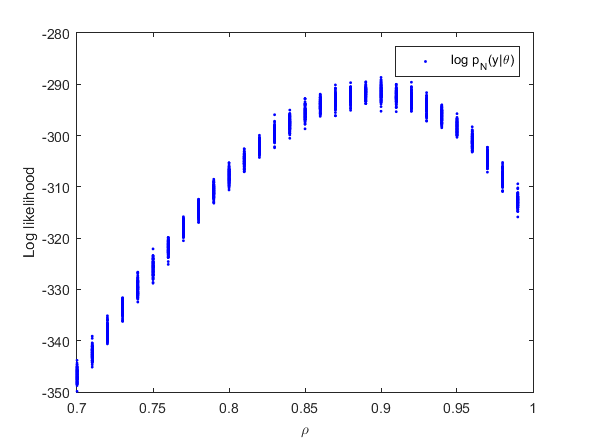
\includegraphics[width=1\textwidth]{tuning_n_rho_varying}
        \caption{$\var(\log \hat{p}_N(y|\theta))$ when $\theta$ varies through $\rho$. Dataset generated from $\mathcal{M}_2$ with $(\rho,\sigma,\nu) = (0.91,1,3)$.}
        \label{tuning_n_rho_varying}
    \end{subfigure}\\
    \begin{subfigure}[1b]{0.49\textwidth}
        \centering
        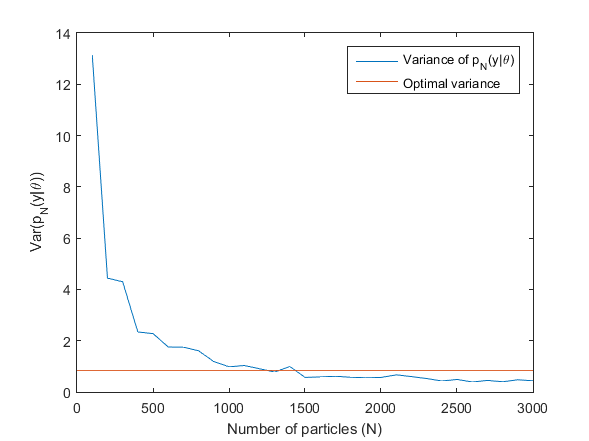
\includegraphics[width=1\textwidth]{tuning_n_optimal_var}
        \caption{$\var(\log \hat{p}_N(y|\bar{\theta}))$ for different values of $N$. Dataset generated from $\mathcal{M}_2$ with $T=1000$ and $(\rho,\sigma,\nu) = (0.91,1,3)$}
        \label{est_var_pn_theta_n}
    \end{subfigure} \\
    \begin{subfigure}[1b]{0.49\textwidth}
        \centering
        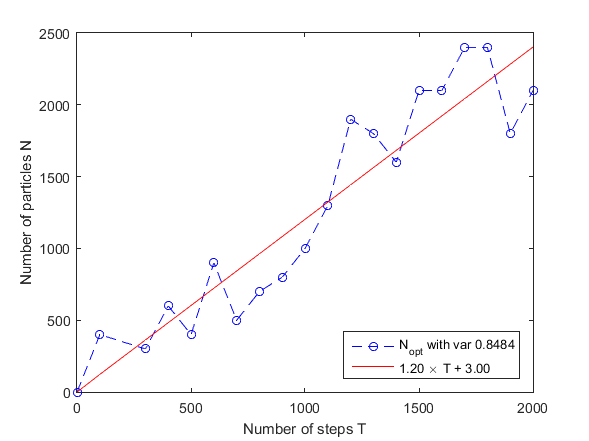
\includegraphics[width=1\textwidth]{n_opt_function_t}
        \caption{Behavior of $N_{opt}$ when $T$ varies}
        \label{n_opt_function_t}
    \end{subfigure}
    \caption{Finding the optimal number of particles $N$}
    %\label{fig:three graphs}
\end{figure}

\chapter{Model Selection and Estimation}

%\section{Validation of the models on Synthetic Data}

In practical applications, the true value of $\theta_{tr}$ is usually unknown and it makes the validation harder. The validation is an important pre-task because it tests the implementation, the choice of the priors and the proposal distributions, and measures the dispersion of the estimator $\hat{\theta}$ to the true value $\theta_{tr}$. The first step involves the sample generation of both the process and the observations $(X_t, Y_t)_{t > 0}$ from a model $\mathcal{M}_x$. We choose an arbitrary realistic value for $\theta_{tr}$. At this point, $x^{tr}_{1:T}$ and $y^{tr}_{1:T}$ are sampled. Each model takes $y^{tr}_{1:T}$ as argument and outputs an estimator $(\hat{x}_{1:T}, \hat{\theta})$. The estimated values are then compared to the true values using some dispersion measures such as the MSE defined by $MSE(\hat{\theta}) = E[ ( \hat{\theta} - \theta_{tr} )^2 ]$. It is also interesting to cross validate the models. The marginal likelihood of the data $p(y^*_{1:T})$ should be maximal for $\mathcal{M}_x$. If the parameters are estimated by another model $\mathcal{M}_y$ say, we should have $p(y^*_{1:T} | \mathcal{M}_x) > p(y^*_{1:T} | \mathcal{M}_y)$ according to the likelihood principles. Every of the 7 models presented in section \ref{sec:sv} has been successfully validated. The source code of the validation is available in the folder \texttt{models} of the repository (Appendix \ref{app:implementation}).

\section{Parameter Estimation on Real Data}

Once the model has been validated, it can be fitted to real world data. The dataset we use is the one presented in section \ref{sec:presentation_data}. The number of steps required in Particle MCMC is taken large enough to ensure that enough samples are available for analysis to form the Bayesian posterior distributions $\mathcal{D}(\theta|y_{1:T})$. Unless stated otherwise, the PMCMC scheme algorithm will loop 10000 times before stopping. The first 1000 samples are discarded for each parameter. This is because the chains require several steps to reach their equilibrium distribution. A component-wise scheme is used to update the parameters, i.e. one by one sequentially. Note that it is possible to parallel this scheme by introducing a bias. However, a more efficient way is to parallel the filter, still with a bias. Both algorithms have been implemented and are available in the appendix. Because the bias has not been rigorously evaluated, a no parallel version was used for the computations. Once the burn-in phase is performed, the mean value $\bar{\theta}$ is selected from the distribution $\mathcal{D}(\theta|y_{1:T})$, as the best estimation for $\theta_{tr}$. Some statistics, moments and confidence intervals can be obtained from $\mathcal{D}(\theta|y_{1:T})$. It is also important to choose correctly the prior distributions $p(\theta)$ and the proposal densities $q(\theta|\theta')$ to maintain a good acceptance rate. \cite{roberts1997} showed that the optimal acceptance rate is 0.234 under quite general conditions. \\
Table \ref{est_appl_params} summarizes such an analysis for model $\mathcal{M}_5$ on the stock APPL in the period Sep, 09 2003 - Jun, 04 2006. Figure \ref{sigma_svm_checks} exposes some checks on the posterior distribution $p(\sigma|y_{1:T}, \mathcal{M}_5)$. The chain mixes well with an acceptance rate 0.180, close to the 0.234 optimal value of \cite{roberts1997}. According to \ref{sigma_svm_2} and \ref{sigma_svm_3}, the posterior distribution seems to be normally distributed, with a skewness of 0.224 and a kurtosis of 2.945. Finally the autocorrelation function of the chain is fast decaying.

\begin{table}[H]
\centering
\begin{tabular}{llll}
Parameter      	& $\rho$ & $\sigma$ & $\beta$ \\ 
\hline
Mean            & 0.9981              & 0.2533             & 0.1475\\
Median          & 0.9982              & 0.2514             & 0.1448\\
Max             & 0.9991              & 0.3941             & 0.2189\\
Min             & 0.9865              & 0.1434             & 0.1100\\
Conf Int (95\%) & [0.9904, 0.9989]    & [0.1822, 0.3345]   & [0.1242, 0.1839]\\
Acceptance Rate & 0.11                & 0.18               & 0.15 \\
MCMC Steps      & 10000               & 10000              & 10000 \\
Burn-in         & 1000                & 1000               & 1000 \\
$p(\theta)$     & $\mathcal{U}[-1,1]$   & $\mathcal{IG}(1,1)$  & $\mathcal{IG}(1,1)$     \\
$q(\theta|\theta')$& $\mathcal{N}(\theta', 0.1^2)$ & $\mathcal{N}(\theta', 0.1^2)$ & $\mathcal{N}(\theta', 0.1^2)$     \\
\hline
\end{tabular}
\caption{Parameters estimation for model $\mathcal{M}_5$. APPL - Sep, 09 2003 - Jun, 04 2006.}
\label{est_appl_params}
\end{table}

\begin{figure}[H]
    \centering
    \begin{subfigure}[t]{0.42\textwidth}
        \centering
        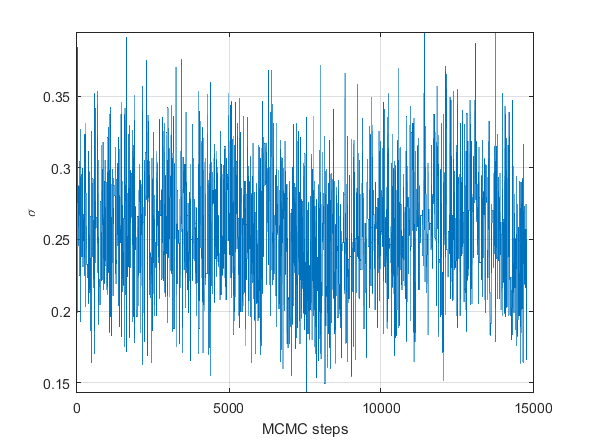
\includegraphics[width=1\textwidth]{sigma_svm/1}
        \caption{MCMC Chain for $\sigma$}
        \label{sigma_svm_1}
    \end{subfigure}
    \begin{subfigure}[t]{0.42\textwidth}
        \centering
        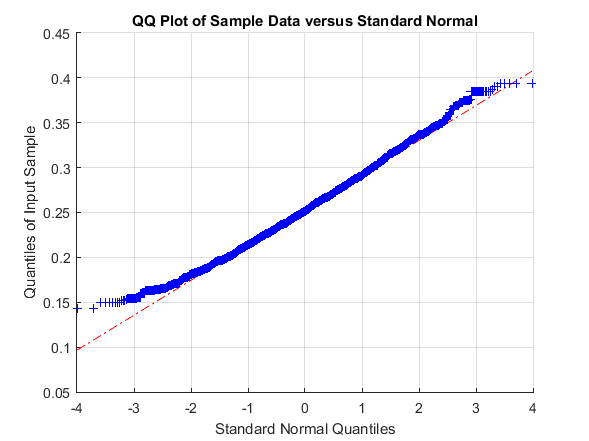
\includegraphics[width=1\textwidth]{sigma_svm/2}
        \caption{QQ Plot - $\sigma$}
        \label{sigma_svm_2}
    \end{subfigure}
    \begin{subfigure}[t]{0.42\textwidth}
        \centering
        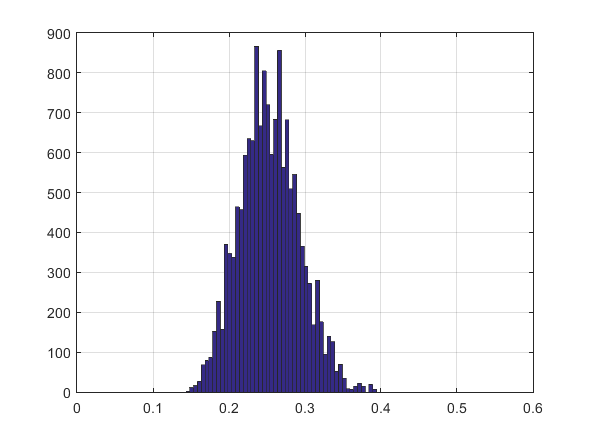
\includegraphics[width=1\textwidth]{sigma_svm/3}
        \caption{Posterior distribution $p(\sigma|y_{1:T})$}
        \label{sigma_svm_3}
    \end{subfigure}
    \begin{subfigure}[t]{0.42\textwidth}
        \centering
        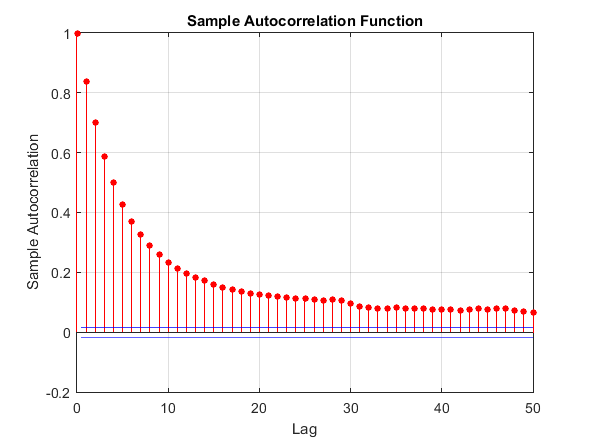
\includegraphics[width=1\textwidth]{sigma_svm/4}
        \caption{Autocorrelation function of $\sigma$}
        \label{sigma_svm_4}
    \end{subfigure}
    \caption{MCMC Checks for $p(\sigma|y_{1:T}, \mathcal{M}_5)$. APPL - Sep, 09 2003 - Jun, 04 2006.}
    \label{sigma_svm_checks}
\end{figure}


\section{Model Selection}
\subsection{Methodology}

The output of the particle filter is an unbiased estimate of $p(y_{1:T}|\theta)$, with the unobserved states integrated out. Although it is very tempting to use it as a measure to compare models, it is always preferred to use the true marginal likelihood $p(y_{1:T})$. According to Bayesian theory, the marginal likelihood for a model $\mathcal{M}$ is defined as

\begin{equation}
p(Y_{1:T} | \mathcal{M}) = \int p(Y_{1:T} | \theta, \mathcal{M}) p(\theta | \mathcal{M}) d\theta
\end{equation}


\cite{gelfand1994} proposed a very general estimate for this marginal likelihood

\begin{equation}
\left(\frac{1}{M} \sum_{i=1}^M \frac{g(\theta_i)}{p(Y_{1:T} | \theta_i) p(\theta_i)}\right)^{-1} \rightarrow p(Y_{1:T}) \text{ as } M \rightarrow \infty
\end{equation}
For this estimator to be consistent, $g(\theta_i)$ must be thin-tailed relative to the denominator. \cite{gelfand1994} argued that for most cases, a multivariate normal distribution $\mathcal{N}(\theta^*, \Sigma^*)$ can be used, where $\theta^*$ and $\Sigma^*$ are equal to the empirical mean and sample unbiased variance, $\theta^* = \frac{1}{M} \sum_{i=1}^M \theta^i$ and $\Sigma^* = \frac{1}{M-1} \sum_{i=1}^M \left(\theta^i - \theta^*\right)\left(\theta^i - \theta^*\right)^T$. \\


The difficulty of this approach resides in its implementation. By its definition, $p(Y_{1:T} | \theta)$ is usually either very close to 0 or very big as the size of the state-space, $T$, grows. The trick here is to consider the sum of the exponential of the logarithms and factorize by the maximum logarithm to avoid rounding errors. For example, let $M = 3$ and assume that the log-terms on the LHS are equal to $-120$, $-121$ and $-122$
\begin{align*}
p(Y_T)^{-1} &= e^{-120} + e^{-121} + e^{-122} \\
- \log p(Y_T) &= \log (e^{-120} ( 1 + e^{-1} + e^{-2})) \\
 \log p(Y_T) &= 120 - \log ( 1 + e^{-1} + e^{-2})) \simeq 119.6
\end{align*}

When $p(Y_T | \mathcal{M_A})$ and $p(Y_T | \mathcal{M_B})$ are estimated, \cite{kass1995} suggests to use twice the logarithm of the Bayes factor for model comparison $2 \log BF_{\mathcal{M_{AB}}}$, where $\mathcal{M_{AB}}$ is the Bayes Factor of $\mathcal{M_A}$ to $\mathcal{M_B}$. \textbf{The evidence of $\mathcal{M_A}$ over $\mathcal{M_B}$ is based on a rule-of-thumb: 0 to 2 not worth more than a bare mention, 2 to 6 positive, 6 to 10 strong, and greater than 10 as very strong.}


\subsection{Results}
\label{sec:model_selection}
It is interesting to see how models perform in practical applications. When it seems pretty obvious that using a leverage can be pertinent according to stylized facts, it seems less evident that the mean of the returns exhibits a stochastic mean proportional to its volatility. The best model is selected on a sample composed of several cointegrated spreads on different periods. The computationally intensive property makes it difficult to test every model for every spread. A sample of 10 spreads is considered beforehand across different sectors such as Energy, Information Technology and Financials. The conclusion is fairly clear on the sample at hand. It turns out that $\mathcal{M}_7$ outperforms all the other models in every situation, in terms of marginal likelihood and AIC. On average, the Kass Factor of $\mathcal{M}_7$ over $\mathcal{M}_6$ is between 2 and 6, showing a positive evidence. The $\mathcal{M}_2$ and $\mathcal{M}_3$ model are respectively ranked third and fourth. This section also introduces an example with detailed explanations about the procedure we used, for a particular spread and a particular stock.
\label{sec:model_selection}
\begin{figure}[H]
    \centering
    \begin{subfigure}[t]{0.49\textwidth}
        \centering
        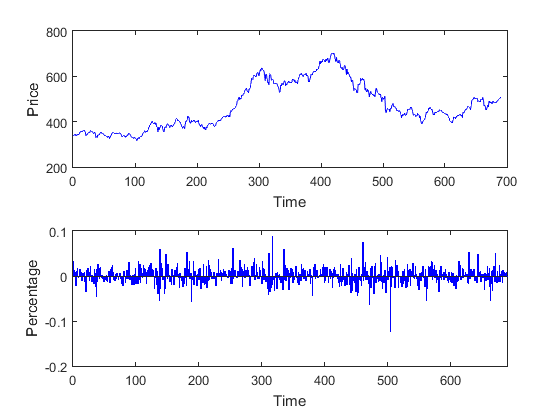
\includegraphics[width=1\textwidth]{apple_2003_2006}
        \caption{APPL stock}
        \label{apple_2003_2006}
    \end{subfigure}
    \begin{subfigure}[t]{0.49\textwidth}
        \centering
        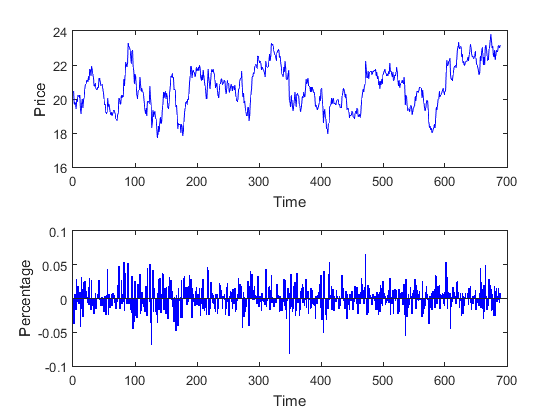
\includegraphics[width=1\textwidth]{spread_amr_crane_2003_2006}
        \caption{Spread AMR CORP - CRANE CO - DOVER CORP. $\beta = (1, -0.0865, -0.3796)$}
        \label{spread_amr_crane_2003_2006}
    \end{subfigure}
    \caption{Stock and Spread. Period is from 09-Sep-2003 to 04-Jun-2006.}
\end{figure}

Both a stock and a spread are considered to see if the results and the inference are in accordance. The stock at hand is Apple (APPL) and the period is Sep, 09 2003 - Jun, 04 2006 (Figure \ref{apple_2003_2006}). The daily returns are computed according to the formula $Y_t = S_t / S_{t-1} - 1$ and are given as input to the stochastic volatility models. We set $N$, the number of particles to 1000 and run the different samplers for $M = 10000$ Metropolis Hastings iterations. After discarding the first 1000 iterations, we collect the final sample and compute the posterior mean $\bar{\theta}$, the posterior median, 95 \% credibility intervals, the log likelihoods that results from the particle filter, the logarithm of the marginal likelihood, the AIC criterion and the M-H acceptance ratio. The model with the highest marginal likelihood is taken as reference and the Bayes factors are computed relatively to this model. Table \ref{estimation_of_sv_appl} and \ref{spread_amr_crane_2003_2006} report estimation of $\theta$ for the stochastic volatility models $(\mathcal{M}_1, ..., \mathcal{M}_7)$. $\log (L)$ is the log marginal likelihood $\hat{p}_N(y| \mathcal{M})$. We find that the Gaussian TFSVL model ($\mathcal{M}_7$) performs best in terms of marginal likelihood and AIC criteria. For the stock case, the Kass factor $2 \log BF$ of SVTFL $\mathcal{M}_7$ versus SVTF $\mathcal{M}_6$ is 2.8 which indicates a positive evidence in favor of the SVTF model and its leverage $\rho$. Compared to the SV with leverage $\mathcal{M}_3$ with one factor, the Kass factor in favor of SVL is 10.0 which is strong evidence. The distribution of the parameters are also fairly concentrated around their means. Overall, the values of $\phi$ are very close to one and confirm strong daily volatility persistence, in accordance to the volatility clustering fact in econometrics. The values of $(\phi_X, \sigma_X)$ and $(\phi_Z, \sigma_Z)$ are very interesting. $\phi_X$ is very close to 1 and $\sigma_X$ is much smaller whereas $\phi_Z$ is almost 0 and $\sigma_Z$ is higher. It seems clear now that the volatility of the returns can be decomposed into two distinct processes: a long-run stochastic trend $(X_t)_{t>0}$ and a process $(Z_t)_{t>0}$ accounting for short-run dynamics. \\

The same procedure was conducted on a spread, composed of three stocks: AMR CORP, CRANE CO and DOVER CORP with associated cointegrating vector $\beta = (1, -0.0865, -0.3796)$. Period is from 09-Sep-2003 to 04-Jun-2006. Table \ref{estimation_of_svm_appl_spr} reports estimation of $\theta$ for the stochastic volatility models $(\mathcal{M}_1, ..., \mathcal{M}_7)$. We find again that the Gaussian TFSVL model ($\mathcal{M}_7$) performs best in terms of the marginal likelihood and AIC criteria. This time, the Kass factor of SVTFL $\mathcal{M}_7$ versus SVTF $\mathcal{M}_6$ is 10.8 which indicates a very strong positive evidence in favor of the SVTF model and its leverage $\rho$. Figure \ref{estimation_of_latent_processes} shows the estimation of the latent processes $(X_t)_{t>0}$ and $(Z_t)_{t>0}$ of model $\mathcal{M}_7$ for the spread. 

\begin{figure}[H]
    \centering
    \begin{subfigure}[t]{0.49\textwidth}
        \centering
        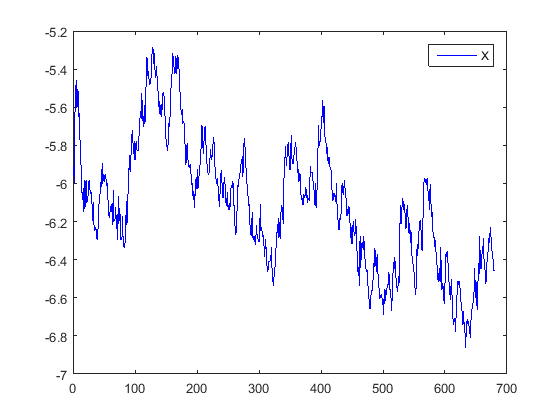
\includegraphics[width=1\textwidth]{est/1}
        \caption{$(X_t)_{t>0}$}
        \label{est_1}
    \end{subfigure}
    \begin{subfigure}[t]{0.49\textwidth}
        \centering
        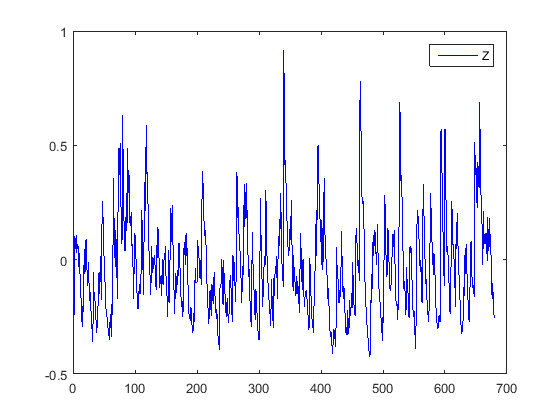
\includegraphics[width=1\textwidth]{est/2}
        \caption{$(Z_t)_{t>0}$}
        \label{est_2}
    \end{subfigure}
    \caption{Estimation of the latent processes $X$, $Z$ and the conditional volatility on returns. Model is $\mathcal{M}_7$. Data is Spr AMR CORP - CRANE CO - DOVER CORP.}
    \label{estimation_of_latent_processes}
\end{figure}

\newpage
\begin{table}[H]
\centering
\begin{tabular}{llllllll}
Parameter        & $\bar{\theta}_{\mathcal{M}1}$ & $\bar{\theta}_{\mathcal{M}2}$ & $\bar{\theta}_{\mathcal{M}3}$ & $\bar{\theta}_{\mathcal{M}4}$ & $\bar{\theta}_{\mathcal{M}5}$ & $\bar{\theta}_{\mathcal{M}6}$ & $\bar{\theta}_{\mathcal{M}7}$\\ 
\hline
$\phi$								                  & 0.9991  & 0.9989 & 0.9960  & 0.9981 & 0.9986 & \\
$\sigma$                                & 0.2395  & 0.1983 & 0.2728  & 0.1694 & 0.2533 & \\
$\beta$                                 & 0.8783  & 0.3705 & 0.1     & 0.2359 & 0.1625 & 0.7427 & 0.6992\\
$\nu$                                   &         & 7.6850 &         & & &\\
$\rho$                                  &         &        & -0.4397 & & & & -0.4178\\
$\psi$                                  &         &        &         & 0.0060 & & \\
$\phi_X$                                &         &        &         & & & 0.9995 & 0.9989\\
$\phi_Z$                                &         &        &         & & & 0.3181 & 0.2477\\
$\sigma_X$                              &         &        &         & & & 0.1222 & 0.1906\\
$\sigma_Z$                              &         &        &         & & & 0.6657 & 0.5219\\
$\log(L)$                               & 2646.3  & 2659.7 & 2660.9  & 2649.2 & 2649.3 & 2664.5 & 2665.9\\
AIC                                     & -5286.6 & -5311.4 & -5313.8 & -5290.4 & -5292.6 & -5319.0 & -5319.8\\
$2 \log \mathcal{BF}(\cdot, \mathcal{M}7)$& 33.9  & 12.4    & 10.0     & 33.4  & 33.2 & 2.8 & 0\\
% $N$                                     & 1000    & 1000   & 1000    & 1000  & 1000 & 1000 & 1000\\
% $T$                                     & 1000    & 1000   & 1000    & 1000  & 1000 & 1000 & 1000\\
% Steps                                   & 10000   & 10000  & 10000   & 10000 & 10000 & 10000 & 10000\\
% Burn-in                                 & 1000    & 1000   & 1000    & 1000  & 1000 & 1000 & 1000\\
\hline
\end{tabular}
\caption{Estimation of the parameters for SV models. Data is APPL.}
\label{estimation_of_sv_appl}
\end{table}

\begin{table}[H]
\centering
\begin{tabular}{llllllll}
Parameter        & $\bar{\theta}_{\mathcal{M}1}$ & $\bar{\theta}_{\mathcal{M}2}$ & $\bar{\theta}_{\mathcal{M}3}$ & $\bar{\theta}_{\mathcal{M}4}$ & $\bar{\theta}_{\mathcal{M}5}$ & $\bar{\theta}_{\mathcal{M}6}$& $\bar{\theta}_{\mathcal{M}7}$\\ 
\hline
$\phi$								                  & 0.9981  & 0.9993 & 0.9986  & 0.9981  & 0.9986 & \\
$\sigma$                                & 0.2238  & 0.1752 & 0.2188  & 0.1694  & 0.2533 & \\
$\beta$                                 & 0.4419  & 0.5722 & 0.4559  & 0.2359  & 0.1625 & 0.3478 & 0.3690\\
$\nu$                                   &         & 7.6850 &         &         &         &\\
$\rho$                                  &         &        & -0.3017 &         &         & & -0.8532\\
$\psi$                                  &         &        &         & 0.0852  &         & \\
$\phi_X$                                &         &        &         &         &         & 0.9995 & 0.9996\\
$\phi_Z$                                &         &        &         &         &         & 0.1926 & 0.7554\\
$\sigma_X$                              &         &        &         &         &         & 0.1268 & 0.0725\\
$\sigma_Z$                              &         &        &         &         &         & 0.4913 & 0.3443\\
$\log(L)$                               & 1792.3  & 1797.8 & 1795.1  & 1793.5  & 1788.5  & 1801.3 & 1806.7\\
AIC                                     & -3578.6 & -3587.6& -3582.2 & -3579.0 & -3571.0 & -3592.6 & -3601.4\\
$2 \log \mathcal{BF}(\cdot, \mathcal{M}7)$& 28.8    & 17.8      & 23.2    & 26.4    & 36.4    & 10.8 & 0 \\
% $N$                                     & 1000    & 1000   & 1000    & 1000    & 1000    & 1000 & 1000\\
% $T$                                     & 689     & 689    & 689     & 689     & 689     & 689 & 689\\
% Steps                                   & 10000   & 10000  & 10000   & 10000   & 10000   & 10000& 10000\\
% Burn-in                                 & 1000    & 1000   & 1000    & 1000    & 1000    & 1000 & 1000\\
\hline
\end{tabular}
\caption{Estimation of the parameters for SV models. Data is Spr AMR CORP - CRANE CO - DOVER CORP.}
\label{estimation_of_svm_appl_spr}
\end{table}

\section{Estimation of the rolling volatility of spreads}
\label{sec:estimation_bollinger_bands_sv}
Once the best Stochastic Volatility model has been selected, $\mathcal{M}_7$ according to section \ref{sec:model_selection} and its parameters being estimated, the volatility of the spread can be approximated. The main idea behind using these stochastic volatility models is to catch the dynamics of the spread through a better estimation of its hidden volatility. According to Definition \ref{spread_def}, a spread is a particular linear combination of assets where each asset price is one observation of a more general process, over a time interval. For a given first order Markovian $N$-process $(\matr{X}_t)_{t>0}$, the returns $y_{1:T}$ modelled by a SV model, are usually of the form $y_t | \matr{x}_t, \theta \sim \mathcal{D} \left( \mu_\theta(t), \sigma_\theta^2(t) \right)$, where $\mathcal{D}$ can represent any suitable distribution in a location-scale family (Definition \ref{location_scale_family}).

\begin{definition}
\label{location_scale_family}
Let $X$ be a random variable taking values in $\mathbb{R}$. For $a \in \mathbb{R}$ and $b > 0$, if $Y = a + b X$ is equal in distribution to $X$, the random variables $X$ and $Y$ belong to the same location-scale family. Examples are the Normal, Cauchy, Uniform, Laplace, GEV and Student $t$ distributions.
\end{definition}

By definition, $Y_t = S_t / S_{t-1} - 1$. We then have
\begin{equation}
S_t | S_{t-1}, \matr{x}_t, \theta \sim \mathcal{D} \left(S_{t-1} \mu_\theta(t)+S_{t-1}, S_{t-1}^2 \sigma_\theta^2(t) \right) \numberthis \label{equation_price_vol}
\end{equation}
where the volatility $\sigma_\theta^2(t)$ and the mean $\mu_\theta(t)$ are known quantities because they only depend on measured quantities ($\matr{x}_{1:t}$ and $S_{t-1}$) at time $t^-$.

In order to estimate the volatility of the spread $(S_t)_{t>0}$, we generate a large number of Monte Carlo paths according to Equation (\ref{equation_price_vol}). Algorithm \ref{rolling_volatility_algo} explains the procedure when the two factors stochastic volatility with leverage model $\mathcal{M}_7$ is considered. The volatility computed in this approach is of the same shape as the one computed in the default Bollinger bands (Equation \ref{bolls_computations}). In the most general case, $M$ paths $\{S_{t,n}\}_{0 < n \leq M, t \in \mathbb{N}}$ are generated from Equation (\ref{equation_price_vol}). Let $f_a : \mathbb{R}^{+M} \rightarrow \mathbb{R}^+$ be a positive-definite aggregating function. The aggregated rolling volatility of lag $p$ for all the $M$ paths is defined as $r\sigma(t,p) = f_a(r\sigma_1(t, p),...,r\sigma_M(t, p))$ for $t >0$. If $f_a$ is simply the sample mean estimator, the equation is simplified to $r\sigma(t,p) = \frac{1}{M}\sum_{i=1}^M r\sigma_i(t, p)$. Depending on the context and on the cross validation phase, $f_a$ can be any measurable function satisfying the conditions above.

\begin{algorithm}
\caption{Rolling volatility computation for model $\mathcal{M}_7$ (TFSVL)}
\label{rolling_volatility_algo}
\begin{algorithmic}[1]
\Procedure{Input}{$x_{1:T}, z_{1:T}, S_{1:T}$, $\theta = \beta$, $M$, $f_a = n^{-1} \sum_{i=1}^M \cdot$}

\For{t from 1 to T}
	\For{i from 1 to M}
		\State Sample the $t^{th}$ value of the $i^{th}$ path, $S_{ti} \sim \mathcal{M}(S_{t-1}, S_{t-1}^2 \beta^2 \exp(x_t + z_t))$
	\EndFor{end}
\EndFor{end}
\For{i from 1 to M}
	\State Compute the default rolling volatility $(r\sigma_i(t))_{t>0}$ for the $i^{th}$ path, $(S_{ti})_{t>0}$
\EndFor{end}

\For{t from 1 to T}
	\State $\displaystyle{r\sigma(t) = n^{-1} \sum_{i=1}^M r\sigma_i(t)}$
\EndFor{end}
\\
\Return $(r\sigma(t))_{t>0}$
\EndProcedure
\end{algorithmic}
\end{algorithm}

\chapter{Statistical Arbitrage Strategies}
Statistical arbitrage conjectures statistical mis-pricings or price relationships that are true in expectation, in the long run when repeating a trading strategy. It describes a variety of automated trading systems which commonly make use of data mining, statistical methods and artificial intelligence techniques. A popular strategy is pairs trade, in which stocks are put into pairs by fundamental or market-based similarities. When one stock in a pair outperforms the other, the poorer performing stock is bought long with the expectation that it will climb towards its outperforming partner, the other is sold short. This hedges risk from whole-market movements. The idea can be easily generalized to $n$ stocks or assets where an asset can be a sector index. The investment strategy we aim at implementing is market neutral, thus we will hold a long and a short position both having approximately the same value in local currency. It is important to understand that the quantity to interest is the difference between the two or $n$ assets, better known as the spread. The purpose is not to trade on assets, but on the spread. The operations to buy or sell the spread are assumed to be atomic, i.e. they have a succeed-or-fail property. The common strategy is to evaluate if the spread is either underpriced or overpriced. A typical is to open a position once the spread deviates far from its long-run equilibrium, and unwind it when it reverts. Dealing with spreads instead of non-stationary assets is beneficial because stationary series are on average more reverting. This approach has the advantage of eliminating the market exposure. \\ 
In this section, two strategies are presented: Bollinger Bands and Z-Score. The first one models a stochastic mean for the spread and stochastic volatility bands to gauge the spread deviation, whereas the second one assumes a fixed non-zero mean and fixed volatility bands.

\section{Bollinger Bands}
\label{sec:bollinger_bands}
Bollinger Bands is a widely used technical volatility indicator invented by John Bollinger in the 1970s which consists of using a moving average $m(t,\cdot)$ of lag $p$ with two volatility bands $B^+(t,\cdot), B^-(t,\cdot)$, above and below it. The computation of the volatility bands involves a windowed standard deviation of lag $p$ (Definition \ref{windowed_volatility}). The shift between the bands and the stochastic mean is proportional to a parameter called $\alpha$. The bands will expand and contract as the price becomes volatile or becomes bound into a tight trading pattern. When prices continually touch the upper bound $B^+(t,\cdot)$, the spread is considered to be overbought. Conversely, when K continually touch the lower band, it is oversold. The indicator is calculated by
\begin{align*}
m_{SMA}(t,p) &= \frac{1}{p}\sum_{j=1}^p S_{t-j} \numberthis \\
m_{EMA}(t,p) &= k \times S_t + (1-k) \times m_{EMA}(t-1,p) \text{, } k = 2/(p+1)\numberthis \\
B^\pm(t,p,\alpha) &= m(t,p) \pm \alpha \underbrace{\sqrt{\frac{1}{p} \sum_{j=1}^p \left(S_{t-j} - m(t,p) \right)^2}}_{r\sigma_B(t,p)} \numberthis \label{bolls_computations}
\end{align*}
where $(S_t)_{t \geq 0}$ is the price of the spread, $p$ is the moving average lag and $\alpha$ is the number of standard deviations to shift the Bollinger bands. According to John Bollinger, the default values are $p = 20$ and $\alpha = 2$. $m_\theta(t)$ is the mid band used as a relative mean value. The exponential moving average (EMA) gives more weights to new values and may be faster to detect opportunities. $B^+_\theta(t)$ and $B^-_\theta(t)$ are respectively the upper and lower bands. Their intrinsic purpose is to measure how far the price deviates from its mean. Under the mild assumption that the returns are normally distributed and independent, approximately 95\% of the prices should appear within the bands when $\alpha = 2$. Figures \ref{bollinger_bands_intro} and \ref{bollinger_bands_intro_2} show different configurations of the Bollinger bands applied to Walt Disney Co NYSE for the year 2002.

\begin{figure}[H]
    \centering
    \begin{subfigure}[t]{0.49\textwidth}
        \centering
        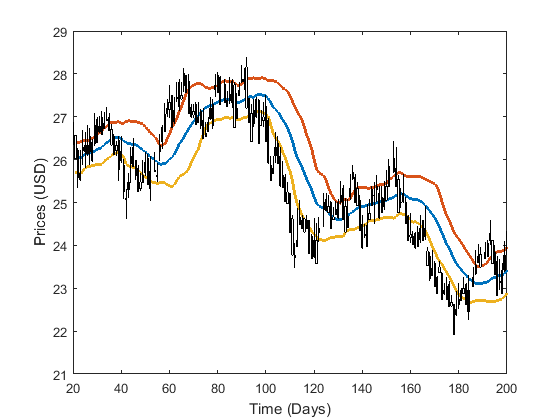
\includegraphics[width=1\textwidth]{bollinger/1}
        \caption{$(p, \alpha) = (20,1.0)$}
        \label{bollinger1}
    \end{subfigure}
    \begin{subfigure}[t]{0.49\textwidth}
        \centering
        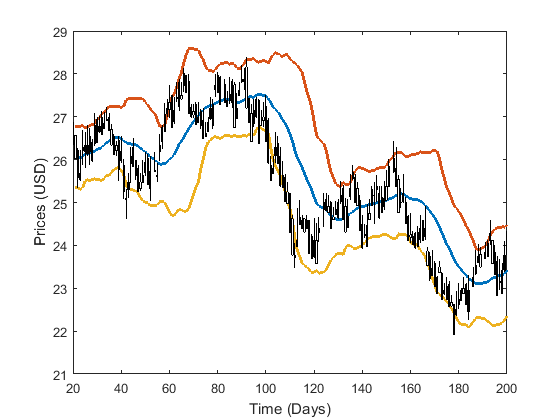
\includegraphics[width=1\textwidth]{bollinger/2}
        \caption{$(p, \alpha) = (20,2.0)$}
        \label{bollinger2}
    \end{subfigure}
    \caption{Bollinger bands strategy applied to Walt Disney Co NYSE for the year 2002. Lag is 20 days. $B^+_\theta$ is red, $B^-_\theta$ yellow and $m_\theta$ navy blue}
    \label{bollinger_bands_intro}
\end{figure}

\begin{figure}[H]
    \centering
    \begin{subfigure}[t]{0.49\textwidth}
        \centering
        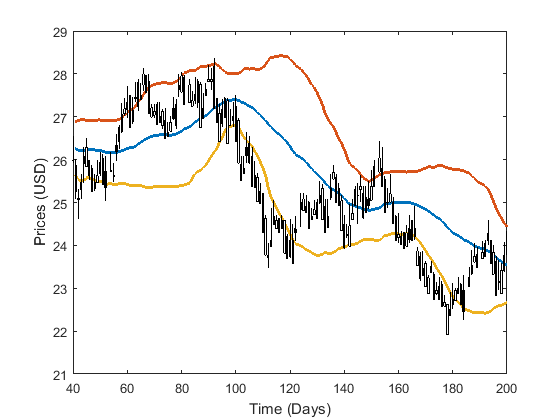
\includegraphics[width=1\textwidth]{bollinger/3}
        \caption{$(p, \alpha) = (40,1.5)$}
        \label{bollinger3}
    \end{subfigure}
    \begin{subfigure}[t]{0.49\textwidth}
        \centering
        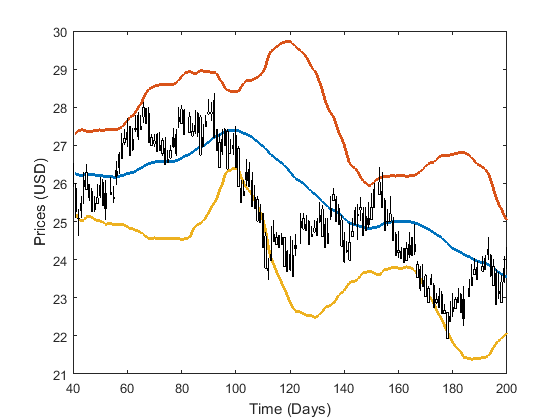
\includegraphics[width=1\textwidth]{bollinger/4}
        \caption{$(p, \alpha) = (40,2.5)$}
        \label{bollinger4}
    \end{subfigure}
    \caption{Example of Bollinger bands strategy applied to Walt Disney Co NYSE for the year 2002. Lag is 40 days. $B^+_\theta$ is red, $B^-_\theta$ yellow and $m_\theta$ navy blue.}
    \label{bollinger_bands_intro_2}
\end{figure}


\section{Building trading signals with the bands}

A trading rule determines the correct timing when to open and close a position. With the Bollinger bands strategy, the rule is:

\begin{itemize}
\item LONG - Open a long position when there is an upward crossing between the spread and the lower band. Unwind this position when there is an upward crossing between the spread and the upper band;
\item SHORT - Open a short position when there is a downward crossing between the spread and the upper band; Unwind this position when there is a downward crossing between the spread and the lower band.
\end{itemize}

\section{Z-score}
Z-score is a strategy based on mean-reverting patterns but unlike the Bollinger bands, Z-score assumed a non-zero constant mean. For this reason, Z-score is only suitable for stationary processes such as spreads. Z-score is dimensionless indicator defined as $z_t = (S_t-\mu_S) / \sigma_S$, where $\mu_S$ and $\sigma_S$ are respectively the unconditional mean and variance of the spread. $z_t$ measures the distance to the long-term mean in units of long-term standard deviation. The basic rule is to open/close a position when the Z-score hits a predefined $n$-quantile of the standard normal distribution $\Phi^{-1}(q_n)$. If the Z-score hits a low threshold, it means that the spread is underpriced and a long position should be opened. When the spread reverts to its mean, the position is unwound. A same reasoning is done for short positions. \cite{caldeira2013} suggested the basic trading strategy signals: Open long position if $z_t \leq \Phi^{-1}(q_{OL}) = -2.00$, open short position if $z_t \geq \Phi^{-1}(q_{OS}) = 2.00$, close short position if $z_t \leq \Phi^{-1}(q_{CS}) = 0.75$ and close long position if $z_t \geq \Phi^{-1}(q_{CL}) = -0.50$. Figure \ref{zscore_graphical_strat} shows the spread $S_t$, the Z-score $z_t$ and the thresholds of the strategy.


\begin{figure}[H]
\centering
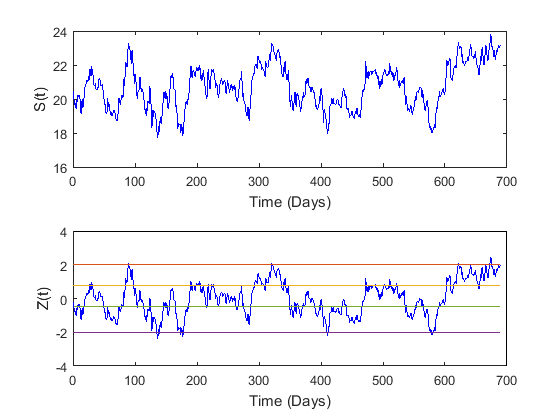
\includegraphics[width = 0.8\textwidth]{zscore/zscore1}
\caption{Spread $S_t$ (defined in section \ref{sec:model_selection}) and its Z-score $z_t$. From top to bottom: $\Phi^{-1}(q_{OS}), \Phi^{-1}(q_{CS}), \Phi^{-1}(q_{CL}), \Phi^{-1}(q_{OL})$.}
\label{zscore_graphical_strat}
\end{figure}

Unlike the Bollinger Bands, the Z-score is highly sensitive to stochastic trends because the mean is assumed to be strictly constant due to the nature of the strategy. In other words, it can be dangerous if the spread loses its cointegrated property and becomes divergent. In practical applications and according to the risk policy of the firm, a stop loss threshold is usually set to avoid any huge losses.

\chapter{Algorithmic Trading Simulation with Model $\mathcal{M}_7$}
Algorithmic trading uses algorithms to drive trading decisions in electronic financial markets. The workflow implemented involves: Preparing the dataset and performing a selection of the suitable tuples satisfying some criteria such as cointegration; Building trading signals for each of the two strategies; Applying parallel for time-efficient backtesting and parameter identification via cross validation; Calculating profit and loss and conducting risk analysis to assess the performance of the strategy.

\section{Cross Validation step}
We use the same dataset as in section \ref{sec:presentation_data}. The whole sample period is divided into sets of length \textbf{two} years. Each set is split into two sets: the in-sample set denoted $\mathcal{I}$ and the out-of-sample $\mathcal{O}$ with a \textbf{2:1} ratio: $(\mathcal{I}_i, \mathcal{O}_i)_{1 \leq i \leq 12}$. Detection of cointegrated tuples, selection of the best tuples and tuning of the Bollinger bands parameters $(p,t,\alpha)$ is done on $\mathcal{I}$. The purpose of $\mathcal{O}$ is to assess the performance of the strategy on unseen data with the parameters computed in the training period. This technique is known as cross validation and is used to avoid overfitting during the calibration. 


\section{General Framework}

The approach consists in ranking the cointegrated tuples based on the best in-sample Sharpe Ratios $\mathcal{SR}$. The first 10 tuples are used to compose the portfolio. The first motivation of considering a portfolio is to lower the volatility associated to each tuple trading by smoothing the net value over time. Only two types of transactions are considered: move into a new position, or unwind a previously opened position. At the end of each trading period, all open positions are closed. Throughout the analysis, we consider 5 point basis of transaction costs. This choice was made for pairs trading in \cite{dunis2010}, \cite{dunis2005} and \cite{alexander2002}. For simplicity, no rental costs are considered for short positions but the capital invested in short selling cannot exceed 50\% of the total capital, either invested or in cash. The asset allocation in the portfolio follows a invested weighting scheme with no dynamic rebalancing. Each tuple is given the same weight and if there are no open positions, the money is not invested and remain as cash in the portfolio. For a particular tuple, the number of open positions is limited to only one per spread. The strategy is self-financing, i.e. profits are reinvested and no deposits or withdrawals are permitted. When a long position is initiated, the first asset is bought with quantity 1 and the remaining assets of the tuple are sold with the respective quantities indicated by the cointegrated vector $\beta$. This same position is closed by selling one unit of the first asset and buying the remaining assets, still in the same proportions. It is assumed that the trader can buy a portion of an asset. \\
The first part of the algorithmic trading part is presented in the next section.

\section{Selection of the cointegrated tuples}

It is common in pair trading to require that the tuples belong to the same sector, for example in \cite{chan2009} and \cite{dunis2010}. Other did not adopt this restriction, for example \cite{caldeira2013}. It is harder but nevertheless possible to bypass this restriction at a greater computational cost when the number of assets $n$ is less than 3. Several methods can be performed to diminish this combinatorial explosion. One is based on correlation. 

\subsection{Complexity Reduction with Correlation}
\label{Complexity_Reduction_with_Correlation}
In the general case, cointegration usually implies correlation but correlation usually doesn't imply cointegration. Spurious regression is a very good example where the reverse is not true. The idea is to filter the uncorrelated tuples to limit the number of candidates for cointegration. This assertion holds because a correlation test is performed much faster than a cointegration test (Table \ref{time_spent_test_bivariate}).

\begin{table}[H]
\centering
\begin{tabular}{ll}
\hline
\multicolumn{1}{|l|}{Test}     & \multicolumn{1}{l|}{Elapsed Time (average)} \\ \hline
Correlation $corr$						 &  0.33 ms \\
Correlation $R^2$ (fast)       &  0.57 ms \\
Johansen                       &  19.08 ms\\
Aug. Dickey Fuller             &  2.33 ms\\
Phillips-Perron                &  3.04 ms\\
\hline
\end{tabular}
\caption{Average time spent to test a bivariate time series $X_t = (x_{t1}, x_{t2})$}
\label{time_spent_test_bivariate}
\end{table}

When it comes to pairs trading, a simple correlation test is enough. When $n \geq 3$, it is preferred to use the multiple correlation coefficient, better known as $R^2$. It can be computed using the vector $c = (r_{x1y}, r_{x2y},...,r_{xNy})^T$ of correlation $r_{xny}$ between the predictor variables $(x_n)_{n \in [1,N]}$ and the target variable $y$, and the correlation matrix $R_{xx}$ of inter-correlations (Equation \ref{rxx}) between predictor variables. It is given by $R^2 = c^T R_{xx}^{-1}c$.

\begin{equation}
R_{xx} =\begin{pmatrix}
r_{x1x1}    & r_{x1x2} & ...  & r_{x1xn}  \\
r_{x2x1}    & \ddots &   & \vdots  \\
\vdots       &   & \ddots &   \\
r_{xnx1}    & \hdots &   & r_{xnxn} \label{rxx} \\
\end{pmatrix} 
\end{equation}
It is worth noting that $R^2$ is order-dependent. To provide convincing evidence of this fact, let's consider a simple example. A regression of $y$ on $x$ and $z$ will in general have a different $R^2$ that will a regression of $z$ on $x$ and $y$. Let $z$ be uncorrelated with both $x$ and $y$ while $x$ and $y$ are linearly related to each other. A regression of $z$ on $y$ and $x$ will yield a $R^2$ of zero, while a regression of $y$ on $x$ and $z$ will yield a strictly positive $R^2$. It means that the ordering inside a tuple has its importance at least from a statistical point of view, as highlighted in Definition \ref{definition_tuple}. This assertion is also true for most cointegrations tests. This notion of ordering is much less obvious from a pure financial point of view. \\

An example is presented with $n=4$. Figure \ref{dist_100_r2_quad} presents the distributions of $R^2$ for each stock sector for quadruples. The period spans from Jan 01, 2012 to May 27, 2013. Most distributions exhibit a bell shape with thin right tails and are therefore candidates for a filtering selection based on an arbitrary threshold $R^2_{th}$. It is worth noting that for $n=4$, each sector has its own threshold $R^2_{th}$. $R^2_{th}$ is usually selected in such a way that we have approximately 20 cointegrated tuples per period.

\begin{figure}[H]
\centering
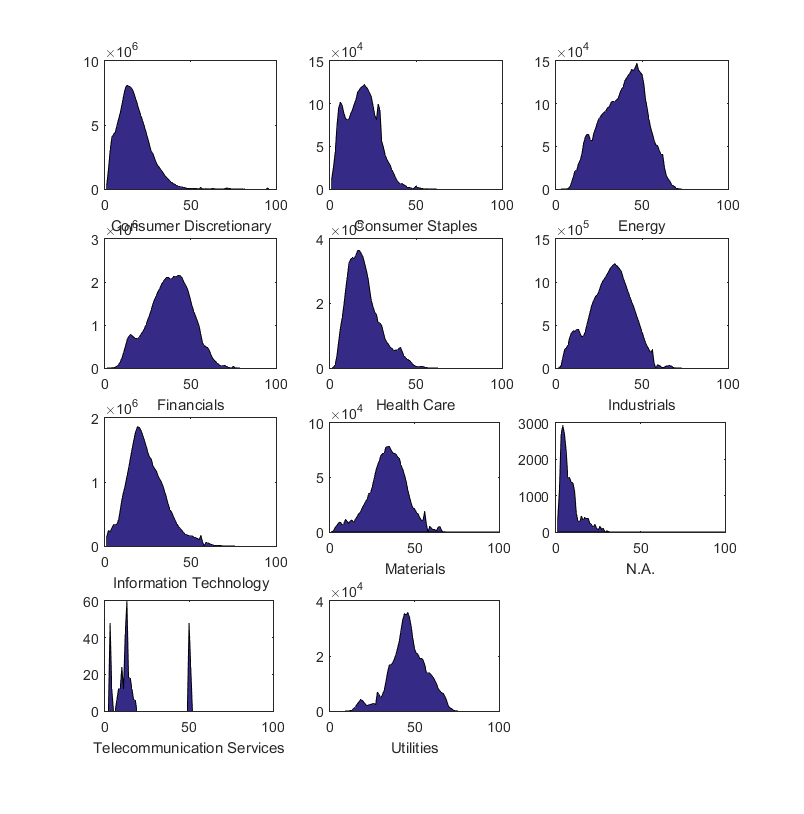
\includegraphics[width = 0.62\textwidth]{R2_ret_Quads_Jan_1_2012_Mar_27_2013}
\caption{Density of $100 \times R^2$ for the quadruples (not all are cointegrated). Period is from Jan 01, 2012 to May 27, 2013}
\label{dist_100_r2_quad}
\end{figure}

\begin{table}[H]
\centering
\begin{tabular}{llll}
\hline
\multicolumn{1}{|l|}{Sector name}     & \multicolumn{1}{|l|}{Count before filtering} & \multicolumn{1}{|l|}{Measure $R_{thr}^2$} & \multicolumn{1}{l|}{Count after filtering} \\ \hline
Consumer Discretionary						 &  165986922 & 0.95 & 15936 \\
Consumer Staples                   &  3025246 & 0.54 & 1074\\
Energy                             &  4651592 & 0.70 & 1536\\
Financials                         &  69777874 & 0.77 & 2730\\
Health Care                        &  7567468 & 0.56 & 2982\\
Industrials                        &  36063822 & 0.70 & 1338\\
Information Technology             & 44043326 & 0.72 & 1080\\
Materials                          & 1972014 & 0.66 & 2070\\
N.A                                & 23232 & 0.21 & 1080\\
Telecommunication Services         & 360 & 0.00 & 360\\
Utilities                          & 760164 & 0.72 & 1290\\
\hline
\end{tabular}
\caption{Correlation filtering on the quadruples from Jan 01, 2012 to May 27, 2013}
\label{corr_quad}
\end{table}
Table \ref{corr_quad} shows the number of quadruples before and after the filtering. $R^2_{thr}$ has been selected in such a way that roughly between 1000 and 10000 quadruples are selected for each sector for cointegration tests. \\
In this case, the assumption of the same sector is almost inevitable but it becomes interesting to question it for triples trading, which is the purpose of the next section.

\subsection{Assumption of the Same Sector}
\cite{chan2009} and \cite{dunis2010} argued that the pairs (and more generally tuples) should belong to the same sector, otherwise the cointegration and the correlation would be purely fortuitous. To check the veracity of this assumption, all the possible cointegrated triples ($n$ = 3) are formed on the whole period of the dataset  - from January, 01 1990 to March, 14 2014 - and the $R^2$ is computed using the methodology exposed in \ref{Complexity_Reduction_with_Correlation}. The cointegrated triples are then sorted according to their $R^2$ from the highest to the lowest value. Each triple is characterized by the sector criteria: \textit{All}, \textit{Partial} or \textit{None}. \textit{All} means the three assets composing the triple belong to the same sector, \textit{Partial} that exactly two belong to the same sector, \textit{None} that all belong to different sectors. As a result, 30418 cointegrated triples were formed. 816 belonged to \textit{All}, 10517 to \textit{Partial} and the remaining 19085 to \textit{None}. Figure \ref{triples_sector_1} shows that for very high $R^2$ on daily returns, almost all the cointegrated triples belong to the same sector. Then for high $R^2$, the proportion of partial triples becomes higher than two other groups until the half of the set. The conclusion is that when the number of selected cointegrating triples or more generally tuples is not very large (less than 500 or 1.5\% here for the whole period), it is reasonable to consider the assumption of the same sector for increased execution speed.

\begin{figure}[H]
    \centering
    \begin{subfigure}[t]{0.49\textwidth}
        \centering
        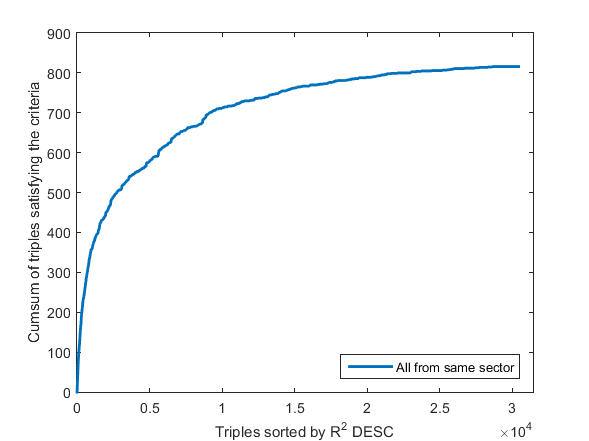
\includegraphics[width=1\textwidth]{triples_sector_0}
        \caption{Cumulative sum of the cointegrated triples from the same sector sorted by $R^2$ from highest to lowest. Period is from 01-Jan-1990 to 14-Mar-2014.}
        \label{triples_sector_0}
    \end{subfigure}
    \begin{subfigure}[t]{0.49\textwidth}
        \centering
        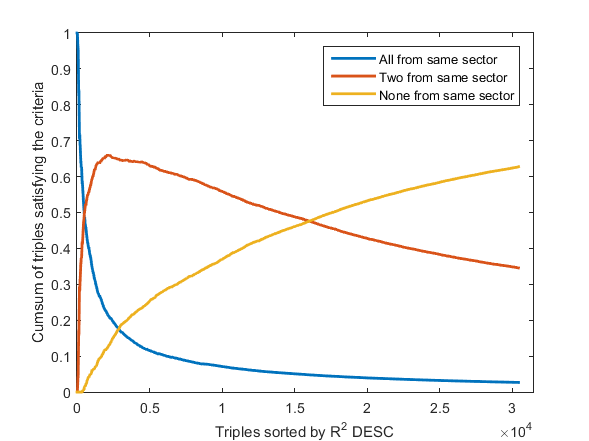
\includegraphics[width=1\textwidth]{triples_sector_1}
        \caption{Distribution of the cointegrated triples sorted by $R^2$ from highest to lowest and regarding their belonging to sectors. Period is from 01-Jan-1990 to 14-Mar-2014.}
        \label{triples_sector_1}
    \end{subfigure}
    \caption{}
    %\label{fig:three graphs}
\end{figure}

\section{Creation of the spreads}
From the candidates of the correlation step, a rigorous testing for cointegration is performed to select the tuples for trading. Algorithm \ref{formation_spread_algorithm} explains the procedure. The result of a test is denoted $h = p_{value} < 0.05$. Values of $h$ equal to 1 indicate rejection of the null hypothesis in favor of the alternative model. Values of $h$ equal to 0 indicate a failure to reject the null.

\begin{algorithm}[H]
\caption{Formation of the Spread}\label{formation_spread_algorithm}
\begin{algorithmic}[1]
\Procedure{Input}{$M$ tuples of size $N$ : $\{ (\matr{X}_i)_{1 < i \leq N} \}_{k}$}
\For{m from 1 to M}
  \State Select the tuple $(\matr{X}_i)_{1 < i \leq N}$ indexed by $m$
  \For{i from 1 to N}
    \State h = Test $\matr{X}_i \sim I(1)$ with an Augmented Dickey-Fuller test
	  \If{h = 1 ($\matr{X}_i \not\sim I(1)$)}
      \State \textbf{Break}
    \EndIf
  \EndFor{end}
  
  \State $[h_1,...,h_N]$ = Perform Johansen Cointegration Test on $(\matr{X}_i)_{1 < i \leq N}$
  \State $r$ = Determine Cointegration Rank of $[h_1,...,h_N]$
  
  \If{$r \neq 1$} //One cointegrating relation is enough
    \State \textbf{Break}
  \EndIf
  
  \For{j from 1 to N} //Order is important in a tuple
    \State Regress $\Delta \matr{X}_j = f((\Delta \matr{X}_i)_{i \neq j})$
    \State Form the spread $\matr{S} = \beta'\matr{X} = \matr{X}_j - \sum_{i\neq j} \beta_i \matr{X}_i$
    \State $h_1$ = Test $\matr{S} \sim I(1)$ with an Augmented Dickey-Fuller test
    \State $h_2$ = Test $\matr{S} \sim RW(\cdot)$ with variance ratio test for random walk
    \If{$h_1 = 1$ \textbf{and} $h_2 = 1$}
      \State $\matr{S}$ is a spread candidate for trading. Add to list $\mathcal{L}(\matr{S})$. 
      \State \textbf{Break} //Success
    \EndIf
    
  \EndFor{end}
  
\EndFor{end}

\\
\Return $(\mathcal{L}(\matr{S}))$
\EndProcedure
\end{algorithmic}
\end{algorithm}

\section{Optimization of the strategy}
\label{sec:optimization_strategy}
Bollinger bands strategy requires to estimate three parameters: the number of periods $p$ to compute the bands, the type $t$ of moving average (EMA or SMA) used in the mid band and $\alpha$ which controls the interval between the volatility bands. John Bollinger suggests $p = 20, \alpha = 2$ and simple moving average as default values. To get the best out of the strategy, a cross validation is performed on the in-sample set $\mathcal{I}$. The criterion of optimization is the in-sample Sharpe Ratio $\mathcal{SR}$. The cross validation parameter space is denoted  $\Omega_{CV} = \mathcal{P}_n \times \mathcal{P}_t \times \mathcal{P}_\alpha$. Complex methods of optimization have also been attempted such as Simulated Annealing. It turns out that an exhaustive search is a serious alternative because of the efforts invested into the parallelization of the task. The exhaustive search provides enhanced visual results and is therefore our recommended choice to reveal the topology of $f(\mathcal{P}_n \times \mathcal{P}_t \times \mathcal{P}_\alpha) \rightarrow \mathbb{R}$.
 
\section{Performance Assessment}
Once the strategy was optimized on $\mathcal{I}$, it can be assessed on the out-sample test $\mathcal{O}$. The performance of the portfolios are examined in terms of cumulative return (CR), variance of returns $\sigma^2$, Sharpe Ratio (SR) and Maximum Drawdown (MDD). Let $y_t$ denote the simple daily return on a particular asset at time $t$. The maximum drawdown (MDD) is defined as the maximum percentage drop incurred from a peak to a bottom up to time $T$. It is the worst possible scenario up to time $T$. By construction, it is higher in absolute values than the maximum loss. Indeed, this is the most pessmistic scenario.

\begin{equation}
MDD(T) = \smash{\displaystyle\max_{s \in (0,T)}} \left[\smash{\displaystyle\max_{s \in (0,T)}} y_t - y_s \right] 
\end{equation}

The Sharpe Ratio (SR) based on daily returns is defined as

\begin{align*}
SR            &=  \frac{\hat{\mu}}{\hat{\sigma}} \text{ where, } \\
\hat{\mu}     &=  252  \times \frac{1}{T} \sum_{t=1}^T y_t \\
\hat{\sigma}  &= \sqrt{252} \times \frac{1}{T} \sum_{t=1}^T (y_t - \bar{\mu})^2 \numberthis \label{sharpe_ratio_def}
\end{align*}


One of the techniques to assess the performance of a strategy is to compare it to the standard Buy and Hold strategy where the holder buys various assets at time $0$ and sell them at time $T$. \cite{gatev2006} also considered a bootstrap approach to generate random trading signals to assess the performance of a strategy over pure randomness. This approach is not discussed here since such a strategy has a negative expectation because of the trading costs.

\chapter{Results}
This chapter is structured in three main parts. Firstly, an example is examined to show some interesting facts about volatility modelling. Next, the cross validation of the Bollinger bands parameters is presented in further details. Finally, the Bollinger bands with and without the complex volatility estimation are compared. Also, the Z-score and the Buy and Hold strategies are considered as a benchmark.
\section{Volatility Modelling of the spread using $\mathcal{M}_7$}
Throughout this section, the same spread $(S_t)_{t>0}$ as that of section \ref{sec:model_selection} is considered. This analysis is not restricted to this particular spread and is valid for any stationary spread and stochastic volatility models. This sections focused on the main points described in section \ref{sec:estimation_bollinger_bands_sv}. The model $\mathcal{M}_7$ is used to estimate the conditional variance $S_t | S_{t-1}, \matr{x}_t, \theta$. From there and from Equation (\ref{equation_price_vol}), $M = 1000$ Monte Carlo trajectories are generated. Figure \ref{fig:generation_of_the_trajectories} shows the generation of the trajectories according to the estimated conditional variance.
\begin{figure}[H]
    \centering
    \begin{subfigure}[t]{0.49\textwidth}
        \centering
        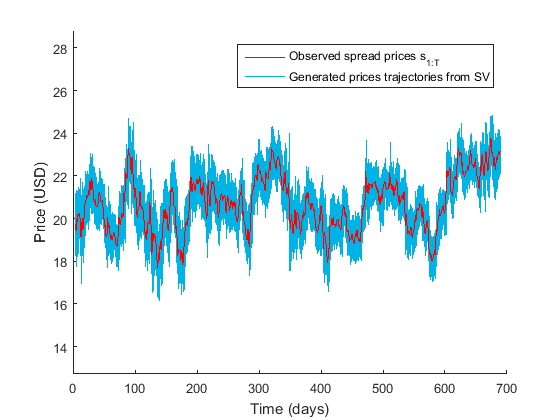
\includegraphics[width=1\textwidth]{model_vol/1}
        \caption{Generation of $M = 1000$ MC prices trajectories with model $\mathcal{M}_7$}
        \label{vol_mod_1}
    \end{subfigure}
    \begin{subfigure}[t]{0.49\textwidth}
        \centering
        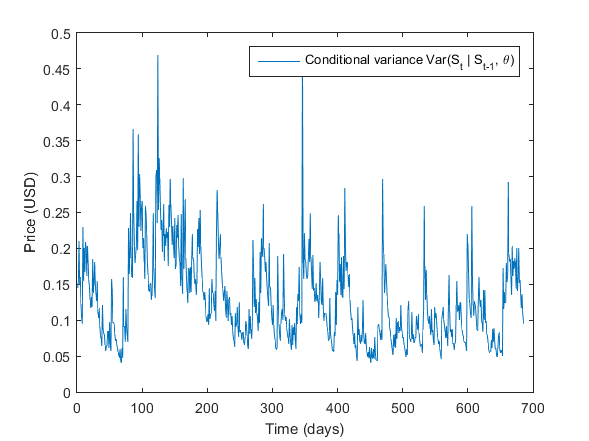
\includegraphics[width=1\textwidth]{model_vol/2}
        \caption{Conditional variance of $S_t | S_{t-1}, \matr{x}_t, \theta$ with model $\mathcal{M}_7$}
        \label{vol_mod_2}
    \end{subfigure}
    \caption{Generation of the trajectories of the spread process $S_t$}
    \label{fig:generation_of_the_trajectories}
\end{figure}

The next step is to compute the rolling volatility for every trajectory. The aggregated function $f_a$ is the sample mean and $r\sigma_{SV}(t)$ is the resulting quantity of this trajectories aggregation. The standard rolling volatility on the observed prices $s_{1:T}$ is denoted $r\sigma_C(t)$. From this point, 90\% and 95\% confidence intervals are derived for every $t \in [1,T]$ using Monte Carlo. The results are presented in Figure \ref{fig:rolling_vol_and_confidence_intervals}\footnote{It is worth noting that the time axis has been truncated to improve readability. The analysis and the conclusions are carried and made on the whole period $[1,T]$.}. It turns out that $r\sigma_C(t)$ is clearly underestimated most of the time. Only 63.9\% of $r\sigma_C(t)$ is contained inside the 0.90 confidence intervals and 78.3\% inside the 0.95 confidence intervals. Moreover, Figure \ref{fig:diff_vol} summarizes the difference $\delta(t) = r\sigma_{SV}(t) - r\sigma_C(t)$. With $E[\delta] = 0.1035$ (USD), the standard volatility estimator is clearly biased.
\begin{figure}[H]
    \centering
    \begin{subfigure}[t]{0.49\textwidth}
        \centering
        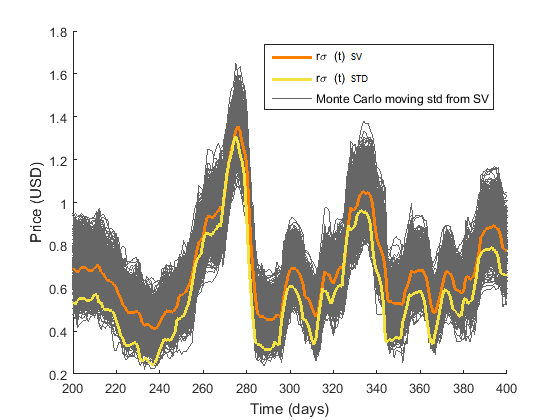
\includegraphics[width=1\textwidth]{model_vol/3}
        \caption{Rolling volatility processes for the generated prices trajectories and the spread prices}
        \label{vol_mod_3}
    \end{subfigure}
    \begin{subfigure}[t]{0.49\textwidth}
        \centering
        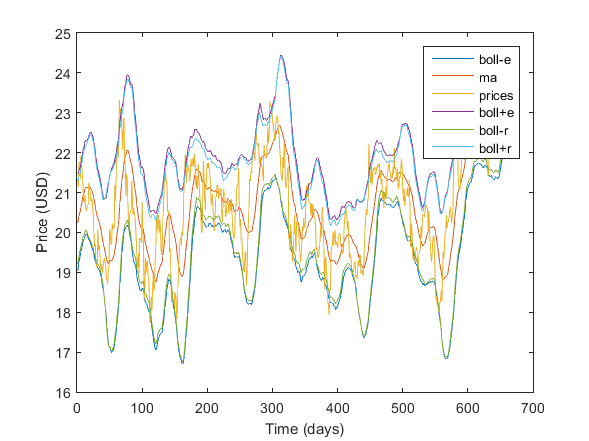
\includegraphics[width=1\textwidth]{model_vol/5}
        \caption{$\delta(t) = r\sigma_{SV}(t) - r\sigma_C(t)$}
        \label{fig:diff_vol}
    \end{subfigure}
    \begin{subfigure}[t]{0.49\textwidth}
        \centering
        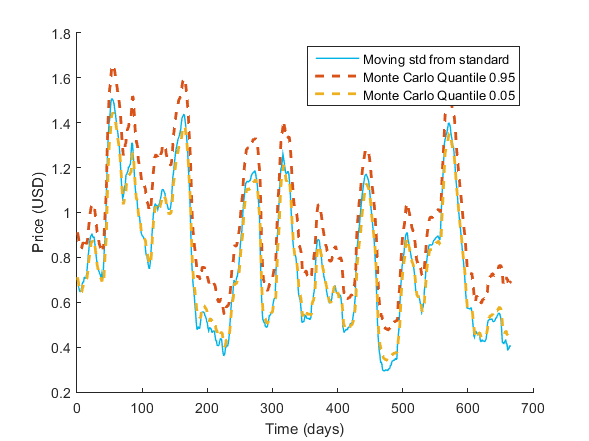
\includegraphics[width=1\textwidth]{model_vol/4}
        \caption{$r\sigma_C(t)$ and 90 \% confidence intervals (MC)}
        \label{vol_mod_4}
    \end{subfigure}
    \begin{subfigure}[t]{0.49\textwidth}
        \centering
        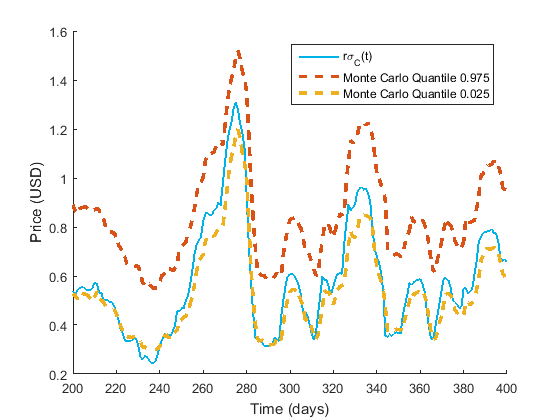
\includegraphics[width=1\textwidth]{model_vol/4_2}
        \caption{$r\sigma_C(t)$ and 95 \% confidence intervals (MC)}
        \label{vol_mod_4}
    \end{subfigure}
    \caption{Generation of the trajectories of the spread process $S_t$}
    \label{fig:rolling_vol_and_confidence_intervals}
\end{figure}

When the rolling volatilities have been estimated, the Bollinger bands can finally be computed. Equation (\ref{bolls_computations}) and (\ref{bolls_computation_sv}) are used to form the bands respectively for the standard and stochastic volatility estimators $r\sigma_C(t)$, $r\sigma_{SV}(t)$.
\begin{equation}
\label{bolls_computation_sv}
B^\pm(t,p,\alpha) = m(t,p) \pm \alpha \cdot r\sigma_{SV}(t,p)
\end{equation}
where the notations of section \ref{sec:bollinger_bands} apply. Figure \ref{fig:bollinger_bands_sma_ema} shows the results for $p=20$ and $\alpha = 2$. The mid band was computed using a simple moving average (SMA) and an exponential moving average (EMA). Not surprisingly, the bands computed with the standard methods are narrower than the ones estimated from stochastic volatility models. It becomes now interesting to see if this volatility can help build more accurate trading signals.

\begin{figure}[H]
    \centering
    \begin{subfigure}[t]{0.49\textwidth}
        \centering
        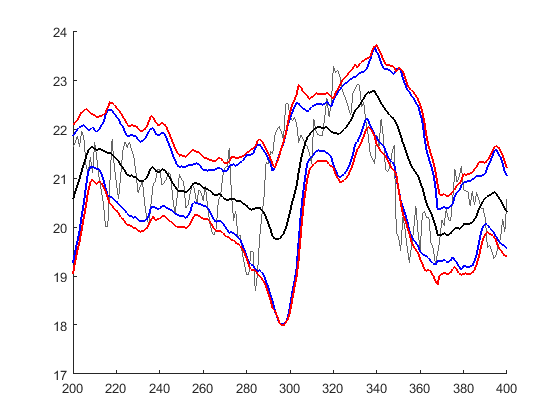
\includegraphics[width=1\textwidth]{model_vol/6}
        \caption{$(p, \alpha, t) = (20, 2.0,\text{EMA})$}
        \label{vol_mod_ema}
    \end{subfigure}
    \begin{subfigure}[t]{0.49\textwidth}
        \centering
        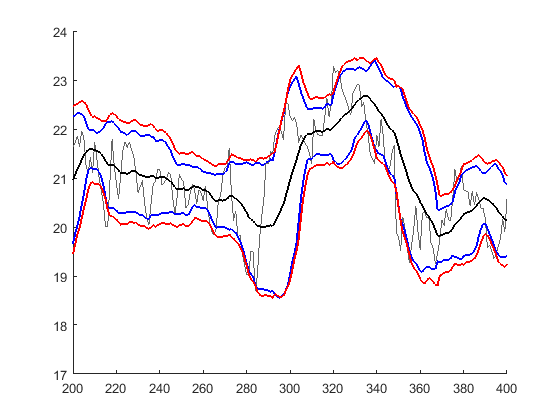
\includegraphics[width=1\textwidth]{model_vol/7}
        \caption{$(p, \alpha, t) = (20, 2.0,\text{SMA})$}
        \label{vol_mod_sma}
    \end{subfigure}
    \caption{Bollinger Bands computed with $r\sigma_C(t)$ (blue) and $r\sigma_{SV}(t)$ (red)}
    \label{fig:bollinger_bands_sma_ema}
\end{figure}

\section{Impact of SV Modelling on Triple Trading}
This section presents the results of the comparisons between Bollinger Bands strategies with and without Stochastic Volatility modelling. The aim is to assess whether using more advanced modelling and model calibration will result to better performance than simple models used often in practice. In the first part, the tuning of the parameters is discarded and the default parameters $(p=20, \alpha = 2, t = \text{SMA})$ recommended by John Bollinger are considered. The cross validation phase could add a bias to the results because we aim to compare the strategies for a fixed $\theta$. The default parameters are widely used in practice among traders and it is pertinent to base the comparison for those values. Later, a cross validation phase is performed to maximize the performance of the best strategy and it is tested against the ZScore and the Buy and Hold strategies. \\

For each $(\mathcal{I}_i)_{1 \leq i \leq 12}$, the cointegrated triples are formed and the 20 best triples are selected based on the $\mathcal{SR}$ criteria on $\mathcal{I}_i$. The model calibration is performed on $\mathcal{I}_i$ for those selected triples. Then, both strategies are tested on the corresponding out-sample set $\mathcal{O}_i$ with the most commonly used parameters and the results are confronted. \\

Table 1 shows the triples used in the strategy from the beginning of 2008 to the end of 2009, especially where the financial crisis of 2008 happened. The formation of the triples is not restricted to the same sector. Of the possible candidates, 5967 passed the cointegration tests described in Algorithm \ref{formation_spread_algorithm}.


\begin{table}[H]
\centering
\begin{tabular}{lllllllllll}
\hline
Stock 1 & Stock 2 & Stock 3 & $\beta_1$ & $\beta_2$ & $\beta_3$ & SRI & SRO & Net Ret. & MDD & Trd\\ \hline
SYY  & PRU  & PTC  & 1.00 & -0.09 & -0.25 & 3.21 & 0.83 & 22991.15 & 0.41 & 287 \\
SYY  & PRU  & PTC  & 1.00 & -0.09 & -0.25 & 3.21 & 0.83 & 22991.15 & 0.41 & 287 \\
JNS  & JDSU  & MDT  & 1.00 & -0.51 & -0.76 & 3.24 & 0.26 & 11255.74 & 0.33 & 242 \\
JNS  & JDSU  & MDT  & 1.00 & -0.51 & -0.76 & 3.24 & 0.26 & 11255.74 & 0.33 & 242 \\
MA  & LSI  & PXD  & 1.00 & -0.23 & -0.24 & 3.24 & 0.34 & 12827.76 & 0.35 & 301 \\
SEE  & SHLD  & TSN  & 1.00 & -0.28 & -0.29 & 3.26 & 0.56 & 11882.95 & 0.25 & 271 \\
MKC  & JNJ  & KSU  & 1.00 & -0.57 & -0.06 & 3.28 & -0.00 & 9989.55 & 0.22 & 287 \\
FII  & FCX  & MSI  & 1.00 & -0.22 & -0.34 & 3.35 & 1.21 & 20997.83 & 0.25 & 250 \\
NSC  & PG  & R  & 1.00 & -0.50 & -0.37 & 3.35 & 1.12 & 32770.77 & 0.48 & 282 \\
LUK  & MAC  & MHK  & 1.00 & -0.31 & -0.43 & 3.37 & 0.20 & 11666.71 & 0.49 & 297 \\
SEE  & SCI  & SHLD  & 1.00 & -0.34 & -0.27 & 3.38 & 1.19 & 14839.25 & 0.15 & 266 \\
SEE  & SCI  & SHLD  & 1.00 & -0.34 & -0.27 & 3.38 & 1.19 & 14839.25 & 0.15 & 266 \\
TIE  & 0772031D  & CVH  & 1.00 & -0.47 & -0.24 & 3.44 & 0.34 & 10992.36 & 0.19 & 288 \\
AMT  & AMP  & CCI  & 1.00 & -0.16 & -0.49 & 3.44 & 1.14 & 15091.08 & 0.14 & 288 \\
MA  & LSI  & OXY  & 1.00 & -0.22 & -0.31 & 3.47 & 0.88 & 24489.13 & 0.31 & 294 \\
FCX  & DIS  & DO  & 1.00 & -0.43 & -0.84 & 3.48 & 0.46 & 19763.68 & 0.74 & 292 \\
ETFC  & DDR  & DE  & 1.00 & -0.31 & -0.47 & 3.51 & 0.87 & 13869.04 & 0.29 & 287 \\
HIG  & BCR  & BRK/B  & 1.00 & -0.65 & -1.58 & 3.55 & 0.23 & 12665.36 & 0.62 & 299 \\
SEE  & SHLD  & UNM  & 1.00 & -0.21 & -0.28 & 3.75 & 1.80 & 16396.51 & 0.09 & 256 \\
SYY  & PNC  & PRU  & 1.00 & -0.04 & -0.13 & 3.90 & 1.07 & 27394.60 & 0.29 & 283 \\
\hline
\end{tabular}
\end{table}

\begin{table}[H]
\centering
\begin{tabular}{lll}
\hline
\multicolumn{1}{|l|}{Ticker}     & \multicolumn{1}{|l|}{Name} & \multicolumn{1}{l|}{Sector}\\ \hline
0772031D UN Equity & QWEST COMMUNICATIONS INTL & N.A. \\
AMP UN Equity & AMERIPRISE FINANCIAL INC & Financials \\
AMT UN Equity & AMERICAN TOWER CORP & Financials \\
BCR UN Equity & CR BARD INC & Health Care \\
BRK/B UN Equity & BERKSHIRE HATHAWAY INC-CL B & Financials \\
CCI UN Equity & CROWN CASTLE INTL CORP & Financials \\
CVH UN Equity & COVENTRY HEALTH CARE INC & N.A. \\
DDR UN Equity & DDR CORP & Financials \\
DE UN Equity & DEERE CO & Industrials \\
DIS UN Equity & WALT DISNEY CO/THE & Consumer Discretionary \\
DO UN Equity & DIAMOND OFFSHORE DRILLING & Energy \\
ETFC UW Equity & E*TRADE FINANCIAL CORP & Financials \\
FCX UN Equity & FREEPORT-MCMORAN COPPER & Materials \\
FII UN Equity & FEDERATED INVESTORS INC-CL B & Financials \\
HIG UN Equity & HARTFORD FINANCIAL SVCS GRP & Financials \\
JDSU UQ Equity & JDS UNIPHASE CORP & Information Technology \\
JDSU UW Equity & JDS UNIPHASE CORP & Information Technology \\
JNJ UN Equity & JOHNSON AND JOHNSON & Health Care \\
JNS UN Equity & JANUS CAPITAL GROUP INC & Financials \\
KSU UN Equity & KANSAS CITY SOUTHERN & Industrials \\
LSI UN Equity & LSI CORP & Information Technology \\
LUK UN Equity & LEUCADIA NATIONAL CORP & Financials \\
MA UN Equity & MASTERCARD INC-CLASS A & Information Technology \\
MAC UN Equity & MACERICH CO/THE & Financials \\
MDT UN Equity & MEDTRONIC INC & Health Care \\
MHK UN Equity & MOHAWK INDUSTRIES INC & Consumer Discretionary \\
MKC UN Equity & MCCORMICK AND CO-NON VTG SHRS & Consumer Staples \\
MSI UN Equity & MOTOROLA SOLUTIONS INC & Information Technology \\
NSC UN Equity & NORFOLK SOUTHERN CORP & Industrials \\
OXY UN Equity & OCCIDENTAL PETROLEUM CORP & Energy \\
PG UN Equity & PROCTER GAMBLE CO/THE & Consumer Staples \\
PNC UN Equity & PNC FINANCIAL SERVICES GROUP & Financials \\
PRU UN Equity & PRUDENTIAL FINANCIAL INC & Financials \\
PTC UQ Equity & PTC INC & Information Technology \\
PTC UW Equity & PTC INC & Information Technology \\
PXD UN Equity & PIONEER NATURAL RESOURCES CO & Energy \\
R UN Equity & RYDER SYSTEM INC & Industrials \\
SCI UN Equity & SERVICE CORP INTERNATIONAL & Consumer Discretionary \\
SEE UN Equity & SEALED AIR CORP & Materials \\
SHLD UQ Equity & SEARS HOLDINGS CORP & Consumer Discretionary \\
SHLD UW Equity & SEARS HOLDINGS CORP & Consumer Discretionary \\
SYY UN Equity & SYSCO CORP & Consumer Staples \\
TIE UN Equity & TITANIUM METALS CORP & N.A. \\
TSN UN Equity & TYSON FOODS INC-CL A & Consumer Staples \\
UNM UN Equity & UNUM GROUP & Financials \\
\hline
\end{tabular}
\end{table}



\section{Gradient and optimization of the Bollinger bands}
This section introduces the results of cross validation on xx spreads from the period xx to xx. The dataset is split into two sets $\mathcal{I}$ and $\mathcal{O}$ with a ratio 2:1. The parameters of the Bollinger bands $(p, \alpha, t)$ are tuned in an exhaustive way, as explained in section \ref{sec:optimization_strategy}. The parameter space is defined as $\Omega_{CV}  = [5,6,...,60] \times \{\text{SMA}, \text{EMA}\} \times [1,1.1,...,2.9,3.0]$ and the topology function $f(\Omega_{CV}) \rightarrow \mathbb{R}$ is the Sharpe Ratio (Definition \ref{sharpe_ratio_def}). The idea is to find regions, not peaks where $f$ has a stable global maximum. As $f$ is multivariate, the idea is to detect a region where $\nabla F(\rho_{max}, \sigma_{max}, t_{max}) = 0$. The gradient $\nabla F$ is defined by
\begin{equation}
\nabla F = \frac{\partial F}{\partial \rho} \vec{i} + \frac{\partial F}{\partial \alpha} \vec{j} + \frac{\partial F}{\partial t} \vec{k}
\end{equation}
In a metric space, $M = (\Omega, d)$, a Borel $\sigma$-algebra $\mathcal{V} = \mathcal{B}(\Omega)$ is a region of a point $p$ if there exists an open ball with center $p$ and radius $r > 0$, such that $B_r(p) = \{\omega \in \Omega | d(\omega, p) < r\}$ is contained in $\mathcal{V}$. To find a suitable global maximum, an exhaustive search is performed for every $\omega \in \Omega$. From this point, the Sharpe ratios are sorted in the descending order $s_1 > s_2 > ... > s_{card(\Omega)}$. The highest Sharpe ratio $s_1$ is considered and its region evaluated with $r=2$. The gradient is then evaluated and checked if it is close to 0. If this is the case, $(p_1, \alpha_1, t_1, s_1)$ is selected. If not, $s_1$ is dropped and $s_2$ is now considered. The procedure goes on until a Sharpe ratio is selected. \\
An example is considered with the spread formed by (NASDAQ:CTSH, NYSE: CTL, CVY:GR) on a period of length($\mathcal{I}$)= 4 years. Figure \ref{fig:sharpe_ratio_topology} introduces the topology of $f$ after the validation on $\mathcal{I}$ and the gradient $\nabla f$. The type of moving average is $t = \{ SMA \}$ and is fixed. At first sight, the region where the global maximum seems to be around $(80,1)$. In this region, the gradient seems to be fairly constant and close to 0.

\begin{figure}[H]
    \centering
    \begin{subfigure}[t]{0.49\textwidth}
        \centering
        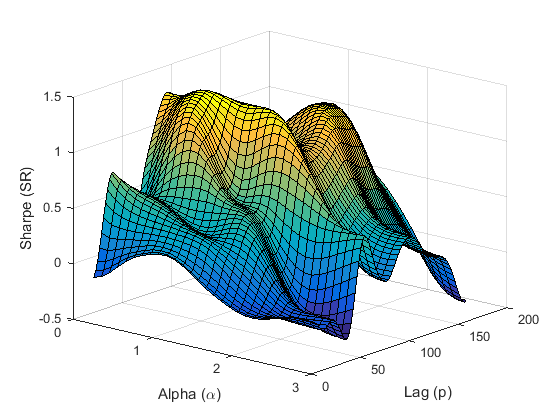
\includegraphics[width=1\textwidth]{surf/1}
        \caption{Topology of $f$ (3D)}
        \label{}
    \end{subfigure}
    \begin{subfigure}[t]{0.49\textwidth}
        \centering
        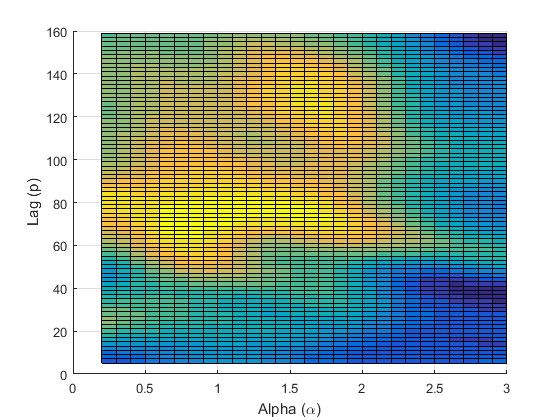
\includegraphics[width=1\textwidth]{surf/2}
        \caption{Topology of $f$ (2D)}
        \label{vol_mod_sma}
    \end{subfigure}
    \begin{subfigure}[t]{0.49\textwidth}
        \centering
        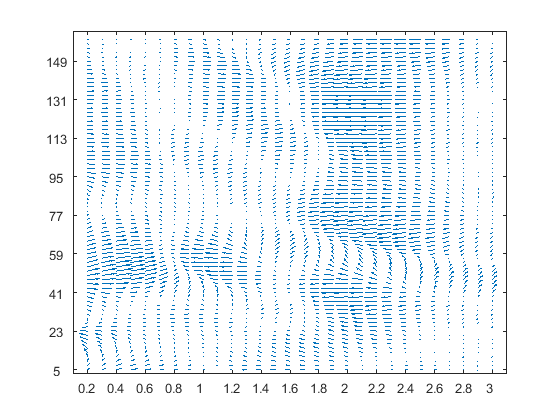
\includegraphics[width=1\textwidth]{surf/3}
        \caption{Gradient $\nabla f$}
        \label{vol_mod_sma}
    \end{subfigure}
    \caption{Detection of the stable global maximum of $f$ with $\nabla f$}
    \label{fig:sharpe_ratio_topology}
\end{figure}

\section{Assessment }

\chapter{Conclusion and Future work}

The strategy is compared to the traditional buy and hold strategy where the investor buys a basket of stocks to reproduce the S\&P500 index and holds it until the end of the period where the position is unwound. Table xx presents the results of both strategies. Figure xx compares the cumulative excess returns and volatility of the strategy with the ones of the SPX index. The portfolio composed of the tuples shows very little volatility compared to the Buy and Hold strategy of the S\&P500 index. The second panel presents the implied volatility of the returns for both strategies computed with a standard stochastic volatility model. The strategy accounts for a low and stable volatility for the whole period. A very low correlation with the market returns attests the market neutral property of the strategy. Table 3 shows the performance year by year of the strategy and it is worth noticing that the excess returns is very high during the crisis where the volatility was very high. As highlighted by \cite{khandani2007} and \cite{avellaneda2010}, the second semester of 2007 and first semester of 2008 were quite complicated for quantitative investment funds. Particularly for statistical arbitrage strategies that experienced significant losses during the period, with subsequent recovery in some cases. Many managers suffered losses and had to sell out their portfolios, not benefiting from the subsequent recovery. We obtain results which are consistent with \cite{khandani2007} and \cite{avellaneda2010} and validate their unwinding theory for the quant fund drawdown. Note that in Figure 3, the proposed pairs trading strategy presented significant losses in the first semester of 2008, starting its recovery in the second semester. \cite{khandani2007} and \cite{avellaneda2010} suggest that the events of 2007-2008 may be a consequence of a lack of liquidity, caused by funds that had to undo their positions. The proposed statistical arbitrage generated average excess returns of 12\% per year in out-of-samples simulations, Sharpe ratio of 1.70, low exposure to the equity market and relatively low volatility and 5pt basis for transaction costs. Even in market crashes, it turns out that the strategy is still highly profitable, reinforcing the usefulness of co-integration in quantitative strategies.

\begin{table}[H]
\centering
\begin{tabular}{lll}
\hline
Summary Statistics of the tuple Trading strategy  			& Strategy & SPX (Buy and Hold)\\ \hline
\# of observations in the sample								& 8844  \\
\# of observations in the training window						& 170 \\
\# of days in the trading period								& 84 \\
\# of trading periods											& 1\\
\# of pairs in each trading period   							& 20\\
\# min of cointegrated pairs in a trading period 				& 35000\\
\# max of cointegrated pairs in a trading period 				& 35000\\
Average annualized return 										& 14.88\% \\
Annualized volatility 											& 6.92\% \\
Annualized Sharpe Ratio 										& 2.54  \\
Largest daily return 											& 2.80\% \\
Lowest daily return 											& -1.94\% \\
Cumulative profit 												& 844.48\%\\
Correlation with the market returns 							& 0.061\\
Skewness														& 1.09\\
Kurtosis 														& 19.89\\
Maximum Drawdown  												& 3.80\% \\
\hline
\end{tabular}
\end{table}

%\begin{figure}[!htb]
%\centering
%\includegraphics[width = 1\textwidth]{img/optimal_lag.pdf}
%\caption{Spread ALCOA INC, AVERY DENNISON CORP, BANK OF NEW YORK MELLON CORP 23-Jun-1995 - 27-Apr-2002}
%\label{fig:1}
%\end{figure}

%\begin{figure}[!htb]
%\centering
%\includegraphics[width = 1\textwidth]{img/profiling_n.pdf}
%\caption{Profiling the number of particles $N$ for $T = 1000$}
%\label{fig:1}
%\end{figure}

%\begin{figure}[!htb]
%\centering
%\includegraphics[width = 1\textwidth]{img/smoothed_var_rho.pdf}
%\caption{Profiling the variance $p_N(y|\theta)$ for several $\rho$ and $N=1000$}
%\label{fig:1}
%\end{figure}

%\begin{figure}[!htb]
%\centering
%\includegraphics[width = 1\textwidth]{img/expnorm.pdf}
%\caption{$\exp \left(\frac{\sigma}{2} \epsilon_R \right) \epsilon_R \text{, } \epsilon_R \sim \mathcal{N}(0,1) \text{, } \sigma > 0$}
%\label{fig:1}
%\end{figure}

\cleardoublepage
\phantomsection
\addcontentsline{toc}{chapter}{\bibname} % Add an entry for the Bibliography in the Table of Contents
%\pagestyle{headings}

\bibliographystyle{abbrvnat} % set the bibliography style
\bibliography{bibtexfile} % generate the bibliography


%\cleardoublepage \fancyhead[L]{APPENDIX}
 % This line declares that you are starting the appendix.
% If you want a single Appendix and want it to be called Appendix instead of Appendix A, the following should work:
%\setcounter{secnumdepth}{-1} %This turns off automatic chapter numbering
%\chapter{Appendix}

\chapter{Appendix}

\section{Implementation}
\label{app:implementation}
All the source code (algorithms, scripts) has been written in Octave using MATLAB 2015a. Since it is open source, it is available to everyone although you have to follow the licenses as defined in the LICENSE file.

\begin{table}[H]
\centering
\begin{tabular}{ll}
\hline
\multicolumn{1}{|l}{Statistics}     & \multicolumn{1}{l|}{} \\ \hline
Repository URL 					   &  \url{https://github.com/philipperemy/Statistical-Arbitrage} \\
Number of commits   			 &  117 \\
Number of files   				 &  195 (MATLAB extension: .m) \\
Codebase   				         &  8727 Lines\\
Author          &  Philippe Remy \\
First commit & May, 19 2015 \\
\hline
\end{tabular}
\caption{Statistics about the repository}
\label{Statistics_repository}
\end{table}

\section{Structure}

\begin{itemize}
\item \texttt{coint/} \\
Files related to cointegration tests and research on spreads (triples and quadruples).
\item \texttt{data/} \\
Contains the datasets.
\item \texttt{filters/} \\
Sequential Monte Carlo filters.
\item \texttt{helpers/} \\
Library of useful functions to manipulate data and perform common computations.
\item \texttt{likelihoods/} \\
Set of functions related to model comparisons.
\item \texttt{models/} \\
Stochastic Volatility model classes used for validation.
\item \texttt{pmcmc/} \\
Generic Particle Markov Chain Monte Carlo framework.
\item \texttt{profiling/} \\
Optimization Functions (number of particles, simulated annealing).
\item \texttt{sandbox/} \\
Experimental folder.
\item \texttt{scripts/} \\
Routine Scripts to run tests, validate models and interact with the git remote repository.
\item \texttt{strategy/} \\
Trading framework gathering strategies (Bollinger Bands, Z Score).
\item \texttt{test/} \\
Test folder. Non regression and validation tests.
\end{itemize}

\section{How to get started} 
The codebase has thousands of lines of code. Therefore, getting started is not easy.
The Particle MCMC framework, implemented for this thesis, is a highly extensible, multi-threaded and customizable framework designed to estimate parameters in non linear state space models. The source code is provided under the MIT license and is available on Github. Contributions are welcome. \\

To define a new PMCMC scheme, the user must inherit from the base abstract class and implement the basic functions. The user must define each of its MC chains as protected member variables, define its priors and proposals distributions and finally link a Particle Filter to the class. The convention used for Particle Filter classes is to return the marginal likelihood and the estimated hidden states.

\section{Proofs}
\label{app:proof}
\begin{proof}
Theorem 6 - \cite{douc2005} \\
For multinomial resampling, the selection indices $I^1,\cdots,I^n$ are conditionally i.i.d. given $\mathcal{F}_t$ and thus the conditional variance is given by
\begin{align*}
\var_M \left[ \frac{1}{n} \sum_{i=1}^n f(\widetilde{\xi_i}) \bigg| \mathcal{F}_t \right] &= \frac{1}{n^2} \var \left[ \sum_{i=1}^n f(\widetilde{\xi_i}) \bigg| \mathcal{F}_t \right] \\
																					  &= \frac{1}{n^2} \sum_{i=1}^n \var \left[ f(\widetilde{\xi_i}) \bigg| \mathcal{F}_t \right] \\
																					  &= \frac{1}{n} \left\{\sum_{i=1}^n \omega_i f^2(\xi_i) - n \left(\sum_{i=1}^n \omega_i f(\xi_i)\right)^2\right\} \numberthis
\end{align*}

An important result for Stratified resampling is
\begin{align*}
E \left[ \sum_{i=1}^n f(\widetilde{\xi_i})  \bigg| \mathcal{F}_t \right] &= E \left[ \sum_{i=1}^n f \circ \xi \circ D_\omega^{inv}(U^i) \bigg| \mathcal{F}_t \right] \\
																  &= \sum_{i=1}^n E \left[ f \circ \xi \circ D_\omega^{inv}(U^i) \bigg| \mathcal{F}_t \right] \\
																  &= n \sum_{i=1}^n \int_{(i-1)/n}^{i/n} f \circ \xi \circ D_\omega^{inv}(u)\text{ }du \numberthis \\
																  &= n \sum_{i=1}^n \omega_i f(\xi_i)
\end{align*}
$U^1,\cdots,U^n$ are still conditionally independent given $\mathcal{F}_t$ for the stratified resampling

\begin{align*}
\var_S \left[ \frac{1}{n} \sum_{i=1}^n f(\widetilde{\xi_i}) \bigg| \mathcal{F}_t \right] &= \frac{1}{n^2} \var \left[ \sum_{i=1}^n f(\widetilde{\xi_i}) \bigg| \mathcal{F}_t \right] \\
																					  &= \frac{1}{n^2} \sum_{i=1}^n \left\{ E \left[ f \circ \xi \circ D_\omega^{inv}(U^i)^2 \bigg| \mathcal{F}_t \right] - E \left[ f \circ \xi \circ D_\omega^{inv}(U^i) \bigg| \mathcal{F}_t \right]^2 \right\}\\
																					  &= \frac{1}{n^2} E \left[ \sum_{i=1}^n f \circ \xi \circ D_\omega^{inv}(U^i)^2 \bigg| \mathcal{F}_t \right] - \frac{1}{n^2} E \left[ f \circ \xi \circ D_\omega^{inv}(U^i) \bigg| \mathcal{F}_t \right]^2 \\
																					  &= \frac{1}{n} \sum_{i=1}^n \omega_i f^2(\xi_i) - \frac{1}{n^2} \sum_{i=1}^n \left[ n \int_{(i-1)/n}^{i/n} f \circ \xi \circ D_\omega^{inv}(u)\text{ }du\right]^2 \\
																					  &= \frac{1}{n} \sum_{i=1}^n \omega_i f^2(\xi_i) - \sum_{i=1}^n \left[ \int_{(i-1)/n}^{i/n} f \circ \xi \circ D_\omega^{inv}(u)\text{ }du\right]^2 \numberthis
\end{align*}

By Jensen's inequality,
\begin{align*}
\sum_{i=1}^n \left[ \int_{(i-1)/n}^{i/n} f \circ \xi \circ D_\omega^{inv}(u)\text{ }du\right]^2 &\geq \left[\sum_{i=1}^n \int_{(i-1)/n}^{i/n} f \circ \xi \circ D_\omega^{inv}(u)\text{ }du\right]^2 = \left[ \sum_{i=1}^n w_i f(\xi_i)\right]^2 \numberthis
\end{align*}
Finally,
\begin{equation}
\var_M \left[ \frac{1}{n} \sum_{i=1}^n f(\widetilde{\xi_i}) \bigg| \mathcal{F}_t \right] \geq \var_S \left[ \frac{1}{n} \sum_{i=1}^n f(\widetilde{\xi_i}) \bigg| \mathcal{F}_t \right] \numberthis
\end{equation}
which closes the proof.
\end{proof}

\section{Cointegration on Foreign Exchange Rates (FX)}

\subsection{Daily prices}

\begin{table}[H]
\centering
\begin{tabular}{llllll}
Currency 1      & Currency 2 & Currency 3 & $\beta_1$ & $\beta_2$ & $\beta_3$ \\ 
\hline
01-Jan-1999 &- 01-Jan-2001 \\
\hline
CADUSD & AUDUSD & EURUSD & 1.000000& -0.169999& 0.041106 \\
CADUSD & AUDUSD & CHFUSD & 1.000000& -0.168860& 0.050292 \\
CADUSD & EURUSD & NZDUSD & 1.000000& 0.042766& -0.136377 \\
CADUSD & EURUSD & CHFUSD & 1.000000& -0.060119& 0.070569 \\
CADUSD & NZDUSD & CHFUSD & 1.000000& -0.137284& 0.055910 \\
\hline
01-Jan-2001 &- 01-Jan-2003 \\
\hline
EURUSD & AUDUSD & GBPUSD & 1.000000& -0.243406& -0.858606 \\
EURUSD & GBPUSD & CADUSD & 1.000000& -0.942491& -0.167773 \\
CHFUSD & GBPUSD & CADUSD & 1.000000& -0.773401& -0.197333 \\
EURUSD & GBPUSD & NZDUSD & 1.000000& -0.843365& -0.251468 \\
EURUSD & GBPUSD & CHFUSD & 1.000000& -0.508161& -0.566663 \\
CHFUSD & GBPUSD & NZDUSD & 1.000000& -0.706983& -0.182011 \\
CHFUSD & CADUSD & EURUSD & 1.000000& -0.045434& -0.871733 \\
\hline
01-Jan-2003 &- 01-Jan-2005 \\
\hline
01-Jan-2005 &- 01-Jan-2007 \\
\hline
EURUSD & AUDUSD & GBPUSD & 1.000000& -0.225093& -0.672751 \\
EURUSD & GBPUSD & ZARUSD & 1.000000& -0.738529& -0.102339 \\
\hline
01-Jan-2007 &- 01-Jan-2009 \\
\hline
01-Jan-2009 &- 01-Jan-2011 \\
\hline
01-Jan-2011 &- 01-Jan-2013 \\
\hline
GBPUSD & AUDUSD & CADUSD & 1.000000& -0.308276& -0.168456 \\
GBPUSD & CADUSD & NZDUSD & 1.000000& -0.268217& -0.227796 \\
GBPUSD & CADUSD & ZARUSD & 1.000000& -0.276975& -0.172995 \\
GBPUSD & CADUSD & CHFUSD & 1.000000& -0.432923& -0.177363 \\
\hline
\end{tabular}
\caption{Cointegration on FX Rates between Jan, 1 1999 and Jan, 1 2013}
\label{coint_fx}
\end{table}



% 
% \section{SVL}
% 
% Again by the Cholesky decomposition, $y_t$ can be written as
% 
% \begin{equation}
% y_t | x_t = \rho \beta \exp(x_t / 2) \epsilon_{X,t} + \beta \exp(x_t / 2) \sqrt{1-\rho^2} Z
% \end{equation}
% The only random quantity here is $Z \sim \mathcal{N}(0,1)$. Both factors on the right hand side are measurable at time $t^-$. Therefore, $y_t|x_t$ is normally distributed
% 
% \begin{equation}
% y_t | x_t \sim \mathcal{N}\left(\mathcal{A} = \rho \beta \exp(x_t / 2) \epsilon_{X,t}, \mathcal{B} = \beta^2 \exp(x_t) (1-\rho^2)\right)
% \end{equation}
% Using the fact that any AR(1) admits an infinite MA representation,
% \begin{align*}
% x_t &= \phi x_{t-1} + \sigma \epsilon_{X,t} \\ 
%   &= \phi(\phi x_{t-2} +\sigma \epsilon_{X,t-1}) + \sigma \epsilon_{X,t} \\
%     &= \sigma \sum_{j=0}^\infty \phi^j \epsilon_{X, t-j} \numberthis
% \end{align*}
% and using this new representation into $\mathcal{A}$ gives
% \begin{align*}
% \mathcal{A} &= \rho \beta \exp(x_t / 2) \epsilon_{X,t} \\
% 			&= \rho \beta \exp \left( \frac{\sigma}{2} \sum_{j=1}^\infty \phi^j \epsilon_{X, t-j}\right) \exp \left( \frac{\sigma}{2} \epsilon_{X,t} \right) \epsilon_{X,t} \\
% 			&= \rho \beta \exp \left( \frac{\phi}{2} x_{t-1}\right) \exp \left( \frac{\sigma}{2} \epsilon_{X,t} \right) \epsilon_{X,t} \numberthis
% \end{align*}
% At time $t-1$, only $\mathcal{C} = \exp \left( \frac{\sigma}{2} \epsilon_{X,t} \right) \epsilon_{X,t}$ is random. Because $\epsilon_{X,t}$ is independent from $x_{t-1}$,
% %%mean(exp(2*rnorm(1000000)))
% %%exp(4^2/8)
% \begin{align*}
% E[\mathcal{A}] &= \rho \beta E\left[\exp \left( \frac{\sigma}{2} \sum_{j=1}^\infty \phi^j \epsilon_{X, t-j}\right)\right] E\left[\exp \left( \frac{\sigma}{2} \epsilon_{X,t} \right) \epsilon_{X,t} \right] \\
% 			   &= \rho \beta E\left[\prod_{j=1}^\infty \exp \left( \frac{\sigma}{2} \phi^j \epsilon_{X, t-j} \right)  \right] E\left[\exp \left( \frac{\sigma}{2} \epsilon_{X,t} \right) \epsilon_{X,t} \right] \\
% 			   &= \rho \beta \prod_{j=1}^\infty E\left[\exp \left( \frac{\sigma}{2} \phi^j \epsilon_{X, t-j} \right)  \right]  E\left[\exp \left( \frac{\sigma}{2} \epsilon_{X,t} \right) \epsilon_{X,t} \right] \numberthis
% \end{align*}
% 
% \begin{align*}
% E\left[\exp \left( \frac{\sigma}{2} \phi^j \epsilon_{X, t-j} \right) \right] &= \frac{1}{\sqrt{2\pi}} \int^{+\infty}_{-\infty} \exp \left(\frac{-x^2}{2} + \frac{\sigma \phi^j}{2} x \right) dx \\
% 																			 &= \left[ \frac{1}{2} \exp \left(\frac{(\sigma\phi^j)^2}{8} \right) erf \left( \frac{2x- \sigma\phi^j}{2 \sqrt{2}} \right) \right]^{+\infty}_{-\infty} \\
% 																			 &= \frac{1}{2} \exp \left(\frac{(\sigma\phi^j)^2}{8} \right) (1 - (-1)) \\
% 																			 &= \exp \left(\frac{(\sigma\phi^j)^2}{8} \right) \numberthis
% \end{align*}
% 
% 
% 
% \begin{align*}
% E\left[\exp \left( \frac{\sigma}{2} \epsilon_{X,t} \right) \epsilon_{X,t} \right] &= \frac{1}{\sqrt{2\pi}} \int^{+\infty}_{-\infty} \exp \left( \frac{-x^2}{2} + \frac{\sigma}{2} x \right) dx \\
% 																				  &= \frac{\sigma}{4} \exp \left(\frac{\sigma^2}{8}\right) \left[ erf \left(\frac{2x-\sigma}{2\sqrt{2}} \right) - \frac{1}{\sqrt{2\pi}}\exp \left(\frac{1}{2} x(\sigma-x) \right) \right]^{+\infty}_{-\infty} \\
% 																				  &= \frac{\sigma}{4} \exp \left(\frac{\sigma^2}{8}\right) (1 - (-1)) \\
% 																				  &= \frac{\sigma}{2} \exp \left(\frac{\sigma^2}{8}\right) \numberthis
% \end{align*}
% Because $\frac{1}{\sqrt{2\pi}}\exp \left(\frac{1}{2} x(\sigma-x) \right) \sim e^{-x^2} \rightarrow 0 \text{ }(x \rightarrow \infty)$. Therefore, 
% \begin{align*}
% 	E[\mathcal{A}] &= \rho \beta \prod_{j=1}^\infty \exp \left(\frac{(\sigma\phi^j)^2}{8} \right) E\left[\exp \left( \frac{\sigma}{2} \epsilon_{X,t} \right) \epsilon_{X,t} \right] \\
% 				   &= \rho \beta \frac{\sigma}{2} \exp \left(\frac{\sigma^2}{8}\right) \prod_{j=1}^\infty \exp \left(\frac{(\sigma\phi^j)^2}{8} \right) \\
% 				   &= \rho \beta \frac{\sigma}{2} \exp \left(\frac{\sigma^2}{8}\right) \exp \left( \frac{\sigma^2}{8} \sum_{j=1}^\infty \phi^{2j} \right) \\
% 				   &= \rho \beta \frac{\sigma}{2} \exp \left(\frac{\sigma^2}{8}\right) \exp \left( \frac{\sigma^2}{8} \left(\frac{1}{1-\phi^{2}} - 1\right)\right) \\
%            &= \rho \beta \frac{\sigma}{2} \exp \left( \frac{\sigma^2}{8} \frac{1}{1-\phi^{2}} \right) \numberthis
% \end{align*}
% 
% %http://www.wolframalpha.com/input/?i=1%2Fsqrt%282*pi%29+exp%28-x%5E2%2F2%2Bs*x%29
% \begin{align*}
% 	E[\mathcal{B}] &= \beta^2 \exp(x_t) (1-\rho^2)\\
% 				   &= \beta^2 (1-\rho^2) E \left[ \exp \left( \sigma \sum_{j=0}^\infty \phi^j \epsilon_{X, t-j}\right) \right]\\
% 				   &= \beta^2 (1-\rho^2) \prod_{j=0}^\infty E\left[\exp \left( \sigma \phi^j \epsilon_{X, t-j} \right)  \right] \\
% 				   &= \beta^2 (1-\rho^2) \prod_{j=0}^\infty \frac{1}{\sqrt{2\pi}}\int^{+\infty}_{-\infty} \exp \left (\sigma \phi^j x - \frac{x^2}{2} \right) dx \\
% 				   &= \beta^2 (1-\rho^2) \prod_{j=0}^\infty \left[\frac{1}{2} \exp \left(\frac{(\sigma \phi^j)^2}{2} \right) erf \left(\frac{x - \sigma\phi^j}{\sqrt{2}}\right)\right]^{+\infty}_{-\infty} \\
% 				   &= \beta^2 (1-\rho^2) \prod_{j=0}^\infty \exp \left(\frac{(\sigma \phi^j)^2}{2} \right) \\
% 				   &= \beta^2 (1-\rho^2) \exp \left( \sum_{j=0}^\infty \frac{(\sigma \phi^j)^2}{2} \right) \\
% 				   &= \beta^2 (1-\rho^2) \exp \left( \frac{\sigma^2}{2} \sum_{j=0}^\infty \phi^{2j} \right) \\
% 				   &= \beta^2 (1-\rho^2) \exp \left( \frac{\sigma^2}{2} \frac{1}{1-\phi^{2}}\right) \numberthis
% \end{align*}
% 
% \section{TFSVL}
% 
% The MA($\infty$) representation of $X_t$ and $Z_t$ are respectively
% \begin{align*}
% X_t &= \sigma_X \sum_{j=0}^\infty \phi_X^j \epsilon_{X, t-j} \numberthis\\
% Z_t &= \sigma_Z \sum_{j=0}^\infty \phi_Z^j \epsilon_{X, t-j} \numberthis
% \end{align*}
% 
% 
% We use the fact that $X_t$ and $Z_t$ are independent for each $t > 0$ i.e. $E[X_t Z_t] = E[X_t] E[Z_t]$.
% 
% From the law of total expectation, $E(Y) = E_Y\left[ E_{Y|X,Z}[Y | X, Z] \right]$. This assertion holds because $(X_t)_{t>0}$ and $(Z_t)_{t>0}$ are AR(1) processes and by their stationary property, $E[|X|],E[|Z|] < \infty$. $Y$ is any random variable, not necessarily integrable but belonging to the same probability space.
% \begin{align*}
% E\left[ Y_t \right] &= E\left[ E[Y_t | x_t, z_t] \right] \\
%                                   &= \rho \beta E\left[\exp \left( \frac{\sigma}{2} \epsilon_{X,t} \right) \epsilon_{X,t} \right] \prod_{i=1}^\infty E\left[\exp \left( \frac{\sigma_X}{2} \phi_X^i \epsilon_{X, t-i} \right)  \right]  \prod_{j=0}^\infty E\left[\exp \left( \frac{\sigma_Z}{2} \phi_Z^j \epsilon_{X, t-j} \right)  \right] \\
%                   &= \frac{\sigma_X}{2} \exp \left(\frac{\sigma_X^2}{8}\right) \exp \left( \frac{\sigma_X^2}{8} \left(\frac{1}{1-\phi_X^{2}} - 1\right)\right) \exp \left( \frac{\sigma_Z^2}{8} \left(\frac{1}{1-\phi_Z^{2}}\right)\right) \numberthis \\
% \end{align*}
% 
% 
% Similarly, the law of total variance is used to compute the unconditional variance of the stochastic process $(Y_t)_{t>0}$. It is assumed that Var($Y) < \infty$ which is the case in practice as the returns are finite almost surely. By definition,
% 
% \begin{equation}
% \var(Y) = \underbrace{E_{X,Z}(Var[Y|X,Z])}_{(1)} + \underbrace{\var_{X,Z}(E[Y|X,Z])}_{(2)}
% \end{equation}
% 
% 
% The term (1) is computed using the same logic as seen for model $\mathcal{M}_3$ with the independence of $X_t$ and $Z_t$ for every $t > 0$.
% \begin{align*}
% E_{X,Z}\left[ \var[Y_t | x_t, z_t] \right] &= \beta^2 (1-\rho^2) \exp \left( \frac{\sigma_X^2}{2} \frac{1}{1-\phi_X^{2}}\right) \exp \left( \frac{\sigma_Z^2}{2} \frac{1}{1-\phi_Z^{2}}\right) \numberthis
% \end{align*}
% 
% 
% The term (2) is rewritten as
% \begin{align*}
% \var_{X,Z} \left[ E[Y_t | x_t, z_t] \right] &= \rho^2 \beta^2 \var \left( \exp \left(\frac{x_t + z_t}{2}\right) \right) \\
%                                                   &= \rho^2 \beta^2 \left( E \left[ \exp \left(x_t + z_t\right) \right] - E \left[ \left( \exp \left(\frac{x_t + z_t}{2}\right) \right) \right]^2 \right) \numberthis
% \end{align*}
% 
% 
% Recall from the calculus for model $\mathcal{M}_3$, $E\left[\exp \left( \frac{\sigma}{2} \phi^j \epsilon_{X, t-j} \right) \right] = \exp \left(\frac{(\sigma\phi^j)^2}{8} \right)$. By a trivial substitution, $\sigma' = 2 \sigma$, $E\left[\exp \left( \sigma' \phi^j \epsilon_{X, t-j} \right) \right] = \exp \left(\frac{(\sigma'\phi^j)^2}{2} \right)$. Therefore,
% 
% \begin{align*}
% (2) &= \rho^2 \beta^2 \left( E [ \exp (x_t) ] E [ \exp (z_t) ] - E \left[ \left( \exp \left(\frac{x_t + z_t}{2}\right) \right) \right]^2\right) \\
%                                                   &= \rho^2 \beta^2 \left( \prod_{j=0}^\infty \exp \left(\frac{(\sigma_X\phi_X^j)^2}{2} \right) \prod_{j=0}^\infty \exp \left(\frac{(\sigma_Z\phi_Z^j)^2}{8} \right) - E \left[ \left( \exp \left(\frac{x_t + z_t}{2}\right) \right) \right]^2\right) \\
%                                                   &= \rho^2 \beta^2 \left( \exp \left( \frac{\sigma_X^2}{2} \frac{1}{1-\phi_X^{2}} \right) \exp \left( \frac{\sigma_Z^2}{2} \frac{1}{1-\phi_Z^{2}} \right) - E \left[ \left( \exp \left(\frac{x_t + z_t}{2}\right) \right) \right]^2\right) \\
%                                                   &= \rho^2 \beta^2 \left( \exp \left( \frac{\sigma_X^2}{2} \frac{1}{1-\phi_X^{2}} \right) \exp \left( \frac{\sigma_Z^2}{2} \frac{1}{1-\phi_Z^{2}} \right) - E \left[ \left( \exp \left(\frac{x_t}{2}\right) \right)\right]^2 E \left[ \left( \exp \left(\frac{z_t}{2}\right) \right)\right]^2\right) \\
%                                                   &= \rho^2 \beta^2 \left( \exp \left( \frac{\sigma_X^2}{2} \frac{1}{1-\phi_X^{2}} \right) \exp \left( \frac{\sigma_Z^2}{2} \frac{1}{1-\phi_Z^{2}} \right) - \exp \left( \frac{\sigma_X^2}{4} \frac{1}{1-\phi_X^{2}} \right) \exp \left( \frac{\sigma_Z^2}{4} \frac{1}{1-\phi_Z^{2}}\right) \right) \numberthis
% \end{align*}
% 
% Finally by adding (1) and (2),
% \begin{multline}
% Var(Y) = \rho^2 \beta^2 \left( \exp \left( \frac{\sigma_X^2}{2} \frac{1}{1-\phi_X^{2}} \right) \exp \left( \frac{\sigma_Z^2}{2} \frac{1}{1-\phi_Z^{2}} \right) - \exp \left( \frac{\sigma_X^2}{4} \frac{1}{1-\phi_X^{2}} \right) \exp \left( \frac{\sigma_Z^2}{4} \frac{1}{1-\phi_Z^{2}}\right) \right) \\ + \beta^2 (1-\rho^2) \exp \left( \frac{\sigma_X^2}{2} \frac{1}{1-\phi_X^{2}}\right) \exp \left( \frac{\sigma_Z^2}{2} \frac{1}{1-\phi_Z^{2}}\right)
% \end{multline}


% \section{Heston}
% \subsection{Simulation of Probability Densities}
% By Ito calculus, and more precisely the Euler-Maruyama method, the Heston stochastic process can be discretized and results in
% 
% \begin{align*}
% S_t &= S_{t-1} + r S_{t-1} dt + \sqrt{V_{t-1}}S_{t-1} \sqrt{dt}Z_t^S \\
% V_t &= V_{t-1} + \kappa(\theta - V_{t-1})dt + \sigma \sqrt{V_{t-1}} \sqrt{dt} Z_t^V
% \end{align*}
% where the innovations $\{Z_t^S\}_{t \geq 0}$ and $\{Z_t^V\}_{t \geq 0}$ are standard normal random variables with correlation $\rho$. The generation is made simple by considering the Cholesky decomposition,
% 
% \begin{align*}
% Z_t^S &= \phi_t^S \\
% Z_t^V &= \rho \phi_t^V + \sqrt{1-\rho^2} \phi_t^V
% \end{align*}
% where $\{\phi_t^S\}_{t \geq 0}$ and $\{\phi_t^S\}_{t \geq 0}$ are independent standard normal random variables.

%%%% http://math.nyu.edu/~atm262/fall06/compmethods/a1/nimalinmoodley.pdf p36

% \section{Stratified Resampling}
% \lstinputlisting{../../filters/resampleStratified.m}
% 
% \section{Generation of the data for validation based on models specifications}
% \lstinputlisting{../../models/HiddenMarkovModel.m}
% \lstinputlisting{../../models/StochasticVolatilityModel.m}
% \lstinputlisting{../../models/StochasticVolatilityModelM.m}
% \lstinputlisting{../../models/StochasticVolatilityModelMA1.m}
% \lstinputlisting{../../models/StochasticVolatilityModelNormalLeverage.m}
% \lstinputlisting{../../models/StochasticVolatilityModelStudent.m}
% \lstinputlisting{../../models/StochasticVolatilityModelTwoFactors.m}
% 
% \section{Bootstrap Particle Filter for Standard SV}
% \lstinputlisting{../../filters/BootstrapParticleFilter.m}
% 
% \section{Bootstrap Particle Filter for Normal Leverage SV}
% \lstinputlisting{../../filters/BootstrapParticleFilter_NormalLeverage.m}
% 
% \section{Bootstrap Particle Filter for Student SV}
% \lstinputlisting{../../filters/BootstrapParticleFilter_Student.m}
% 
% \section{Bootstrap Particle Filter for SVM}
% \lstinputlisting{../../filters/BootstrapParticleFilter_SVM.m}
% 
% \section{Bootstrap Particle Filter for SVMA1}
% \lstinputlisting{../../filters/BootstrapParticleFilter_SVMA1.m}
% 
% \section{Bootstrap Particle Filter for Two Factors SV}
% \lstinputlisting{../../filters/BootstrapParticleFilter_TwoFactors.m}
% 
% \section{Bootstrap Particle Filter for Two Factors SV with Leverage}
% \lstinputlisting{../../filters/BootstrapParticleFilter_TwoFactorsCor.m}
% 
% \section{Particle Markov Chain Monte Carlo (Abstract Class)}
% \lstinputlisting{../../pmcmc/ParticleMarkovChainMonteCarlo.m}
% 
% \section{Particle Markov Chain Monte Carlo Standard Stochastic Volatility Model}
% \lstinputlisting{../../pmcmc/ParticleMarkovChainMonteCarloSV.m}
% 
% \section{Particle Markov Chain Monte Carlo SVM}
% \lstinputlisting{../../pmcmc/ParticleMarkovChainMonteCarloSVM.m}
% 
% \section{Particle Markov Chain Monte Carlo SVMA1}
% \lstinputlisting{../../pmcmc/ParticleMarkovChainMonteCarloSVMA1.m}
% 
% \section{Particle Markov Chain Monte Carlo SV Normal Leverage Model}
% \lstinputlisting{../../pmcmc/ParticleMarkovChainMonteCarloSVNormalLeverageBeta.m}
% 
% \section{Particle Markov Chain Monte Carlo SV Student Model}
% \lstinputlisting{../../pmcmc/ParticleMarkovChainMonteCarloStudentBetaSV.m}
% 
% \section{Particle Markov Chain Monte Carlo SV Two Factors}
% \lstinputlisting{../../pmcmc/ParticleMarkovChainMonteCarloSVTwoFactorsBeta.m}
% 
% \section{Particle Markov Chain Monte Carlo SV Two Factors with Leverage}
% \lstinputlisting{../../pmcmc/ParticleMarkovChainMonteCarloSVTwoFactorsBetaCor.m}
% 
% \section{Bayes Factor - Kass and Raftery}
% \lstinputlisting{../../likelihoods/BayesFactor.m}
% 
% \section{Marginal Likelihood $p(y_{1:T})$ - Gelf and Dey}
% \lstinputlisting{../../likelihoods/GelfandDey_LogMarginalY.m}
% 
% \section{Spread Finder}
% \lstinputlisting{../../coint/deepsearch/SpreadFinder.m}
% 
% \section{Spread Constructor}
% \lstinputlisting{../../coint/deepsearch/SpreadConstructor.m}
% 
% \section{Build Order}
% \lstinputlisting{../../coint/deepsearch/SpreadBuildOrder.m}
% 
% \section{Trading Strategy}
% \lstinputlisting{../../strategy/SimpleTradingStrategy.m}
% 
% \section{Trading Strategy Cross Validation}
% \lstinputlisting{../../strategy/SimpleTradingStrategyCV.m}
% 
% \section{Reversion Frequency Calculator}
% \lstinputlisting{../../helpers/ReversionFrequencyCalculator.m}
% 
% \section{Crossing Points Calculator}
% \lstinputlisting{../../strategy/CrossingPointsCalculator.m}
% 
% \section{Computation of the returns}
% \lstinputlisting{../../helpers/Compute_Returns.m}
% 
% \section{$R^2$ computation for quadruples (efficient implementation)}
% \lstinputlisting{../../helpers/Compute_R_2.m}
% 
% \section{Windowed Standard Volatility (Rolling)}
% 
% This code was written by John D'Errico (2005) and is under the BSD License. \\
% \url{http://www.mathworks.com/matlabcentral/fileexchange/9428-movingstd-x-k-windowmode-}
% \lstinputlisting{../../helpers/movingstd.m}
% 
% \section{Main}
% \lstinputlisting{../../strategy/Main2.m}

\end{document}
